\documentclass{article}
\usepackage{xeCJK}
% if you need to pass options to natbib, use, e.g.:
%\PassOptionsToPackage{numbers, compress}{natbib}
% before loading nips_2017
%
% to avoid loading the natbib package, add option nonatbib:
% \usepackage[nonatbib]{nips_2017}

\usepackage[final]{nips_2017}

% to compile a camera-ready version, add the [final] option, e.g.:
% \usepackage[final]{nips_2017}

\usepackage[utf8]{inputenc} % allow utf-8 input
\usepackage[T1]{fontenc}    % use 8-bit T1 fonts
\usepackage{hyperref}       % hyperlinks
\usepackage{url}            % simple URL typesetting
\usepackage{booktabs}       % professional-quality tables
\usepackage{amsfonts}       % blackboard math symbols
\usepackage{nicefrac}       % compact symbols for 1/2, etc.
\usepackage{microtype}      % microtypography
\usepackage{bm}             % bold in math
\usepackage{graphicx}       % images
\usepackage{algorithm}      % algorithm
\usepackage[noend]{algpseudocode} % algorithm
\usepackage{caption}        % captionof
\usepackage{array}          % thick column hline
\usepackage{booktabs}       % table style
\usepackage{pbox}           % table line break
\usepackage{subcaption}     % multiple figures
\usepackage{listings}
\usepackage{xcolor}
\usepackage{tikz}
\usepackage{amsmath}
\definecolor{mygreen}{rgb}{0,0.6,0}
\definecolor{mygray}{rgb}{0.5,0.5,0.5}
\definecolor{mymauve}{rgb}{0.58,0,0.82}
\definecolor{codeBkg}{rgb}{0.85,0.85,0.85}

\lstset{ 
	backgroundcolor=\color{codeBkg},   % choose the background color; you must add \usepackage{color} or \usepackage{xcolor}; should come as last argument
	basicstyle=\footnotesize,        % the size of the fonts that are used for the code
	breakatwhitespace=false,         % sets if automatic breaks should only happen at whitespace
	breaklines=true,                 % sets automatic line breaking
	captionpos=b,                    % sets the caption-position to bottom
	commentstyle=\color{mygreen},    % comment style
	deletekeywords={...},            % if you want to delete keywords from the given language
	escapeinside={\%*}{*)},          % if you want to add LaTeX within your code
	extendedchars=true,              % lets you use non-ASCII characters; for 8-bits encodings only, does not work with UTF-8
	frame=no,	                   % adds a frame around the code
	keepspaces=true,                 % keeps spaces in text, useful for keeping indentation of code (possibly needs columns=flexible)
	keywordstyle=\color{blue},       % keyword style
	language=Octave,                 % the language of the code
	morekeywords={*,...},            % if you want to add more keywords to the set
	numbers=left,                    % where to put the line-numbers; possible values are (none, left, right)
	numbersep=5pt,                   % how far the line-numbers are from the code
	numberstyle=\tiny\color{mygray}, % the style that is used for the line-numbers
	rulecolor=\color{black},         % if not set, the frame-color may be changed on line-breaks within not-black text (e.g. comments (green here))
	showspaces=false,                % show spaces everywhere adding particular underscores; it overrides 'showstringspaces'
	showstringspaces=false,          % underline spaces within strings only
	showtabs=false,                  % show tabs within strings adding particular underscores
	stepnumber=1,                    % the step between two line-numbers. If it's 1, each line will be numbered
	stringstyle=\color{mymauve},     % string literal style
	tabsize=4,	                   % sets default tabsize to 2 spaces
	title=\lstname                   % show the filename of files included with \lstinputlisting; also try caption instead of title
}

\title{高级量化交易技术}

\hypersetup{
    colorlinks = true,
}
\makeatletter
\def\BState{\State\hskip-\ALG@thistlm}
\makeatother
\floatname{algorithm}{Procedure}
\renewcommand{\algorithmicrequire}{\textbf{Input:}}
\renewcommand{\algorithmicensure}{\textbf{Output:}}

\newcolumntype{?}{!{\vrule width 3pt}}

\author{
  闫涛 \\
  %% examples of more authors
  %% \And
  %% Nicholas Frosst \\
  %% Affiliation \\
  %% Address \\
  %% \texttt{email} \\
  %% \AND
  %% Geoffrey E. Hinton \\
  科技有限公司\\
  北京 \\
  \texttt{\{yt7589\}@qq.com} \\
  %% Affiliation \\
  %% Address \\
  %% \texttt{email} \\
  %% \And
  %% Coauthor \\
  %% Affiliation \\
  %% Address \\
  %% \texttt{email} \\
  %% \And
  %% Coauthor \\
  %% Affiliation \\
  %% Address \\
  %% \texttt{email} \\
}
\date{March 2018}

% \usepackage{natbib}
% \usepackage{graphicx}

\begin{document}






\maketitle
\begin{center}
\Large \textbf{第1章} \quad \textbf{时间序列基本特性}
\end{center}
\begin{abstract}
在本章中我们将讨论时间序列的基本特性,包括自相关性和平稳性。
\end{abstract}
\section{时间序列基本特性}
时间序列的自相关性是指时间序列过去与未来存在某种关系,是我们时间序列预测的基础。主要用自协方差函数(Autocovariance Function, AF)、自相关系数函数(Autocorrelation Coefficent Function, ACF)和偏自相关系数函数(Partial Autocorrelation Coefficient Function, PACF)来描述。
\subsection{随机变量统计量}
随机变量X其取值为$x$的均值定义为:
\begin{equation}
E(x) = \mu
\label{e000001}
\end{equation}
方差定义为:
\begin{equation}
\sigma ^{2} (x) = E\bigg[ \big( x - \mu \big)^{2} \bigg]
\label{e000002}
\end{equation}
其中$\sigma (x)$为标准差。
对于两个随机变量$x$和$y$,其协方差可以定义为:
\begin{equation}
\sigma (x, y) = E\bigg[ \big( x - \mu _{x} \big) \big( y - \mu _{y} \big) \bigg]
\label{e000003}
\end{equation}
在实际应用中,我们不可能知道真实的均值,只能使用统计量,因此协方差可以定义为:
\begin{equation}
Cov(x, y) = \frac{1}{n-1} \sum_{i=1}^{n} (x_{i} - \bar{x})(y_{i} - \bar{y})
\label{e000004}
\end{equation}
随机变量$x$和$y$的相关系数定义为:
\begin{equation}
\rho(x,y)=\frac{E[(x-\mu_{x})(y-\mu_{y})]}{\sigma _{x} \sigma _{y}}=\frac{\sigma(x,y)}{\sigma _{x} \sigma _{y}}
\label{e000005}
\end{equation}
采用统计量的表示方法为:
\begin{equation}
Cor(x,y)=\frac{Cov(x,y)}{std(x) \times std(y)}
\label{e000006}
\end{equation}
以上我们讨论的都是不同随机变量之间的关系,对于时间序列来说,我们可以把从不同时间点开始的子时间序列,视为不同的随机变量,那么我们就可以定义自协方差、自相关系数函数和偏自相关系数函数了。\newline
\subsection{时序序列平稳性}
时序信号$x_{t}$的均值定义为:
\begin{equation}
E(x_{t})=\mu (t)
\label{e000007}
\end{equation}
时间序列的均值与所考虑的时间点有关。我们可以把时间序列上每个时间点都视为一个独立的时间变量,但是对于时间序列而言,每个时间点的随机变量只有一个观测值,怎么求出均值呢?在实际应用中,我们会将时间序列中的趋势信号(上涨或下跌)、季节性信号等从时间序列中去除掉,对于剩下的残差序列,我们可以视为其各个时间点上的随机变量的均值是不变的,于是就可以使用下面的公式来计算均值:
\begin{equation}
\bar{x}=\frac{1}{N} \sum_{t=1}^{N}x_{t}
\label{e000008}
\end{equation}
由此我们引入平稳时间序列的概念,对于平稳时间序列,其各个时间点上对应的随机变量的均值相等。
时间序列的方差可以定义为:
\begin{equation}
\sigma ^{2}(t)=E[(x_{t}-\mu _t)^{2}]
\label{e000009}
\end{equation}
根据上面平稳时间序列的定义,各个时间点对应的随机变量的均值不变,则式\ref{e000009}可以化间为:
\begin{equation}
\sigma ^{2}(t)=E[(x_{t}-\mu)^{2}]
\label{e000010}
\end{equation}
我们同时规定,平稳时间序列各个时间点对应的随机变量的方差也不变,则\ref{e000010}可进一步化简为:
\begin{equation}
Var(x_{t})=\frac{1}{N-1} \sum_{t=1}{N} (x_t - \bar{x})^{2}
\label{e000011}
\end{equation}
\subsection{自协方差}
在讨论自协方差之前,我们首先要定义二阶平稳性。根据上一节定义,平稳时间序列是指各个时间点对应的随机变量的均值和方差相同。二阶平稳性是指在这一基础上,不同时间点对应的随机变量的相关系数只与时间相隔(lag)相关。注意:以下我们讨论的各种性质,均以此为前提。
对于lag=k的自协方差定义为:
\begin{equation}
C_{k}=E[(x_{t} - \mu)(x_{t+k} - \mu)]
\label{e000012}
\end{equation}
\subsection{自相关系数函数ACF}
由于自协方差的大小与随机变量的大小有关,无法准确衡量其间的关系,因此我们引入自相关系数函数ACF:
\begin{equation}
\rho _{k} = \frac{C_{k}}{\sigma ^{2}}
\label{e000013}
\end{equation}
由定义可知:
\begin{equation}
\begin{aligned}
\rho _{0} = \frac{C_{0}}{\sigma ^{2}} = \frac{E[(x_{t} - \mu)(x_{t} - \mu)]}{\sigma ^{2}} \\
= \frac{E[(x_{t} - \mu)^{2}]}{\sigma ^{2}} = \frac{\sigma ^{2}}{\sigma ^{2}} = 1\\
\end{aligned}
\label{e000014}
\end{equation}
在实际应用中,我们都是处理的离散数据点,则自协方差可以定义为:
\begin{equation}
c_{k}=\frac{1}{N}\sum_{t=1}^{N}(x_{t}-\bar{x})(x_{t+k} - \bar{x})
\label{e000015}
\end{equation}
自相关系数函数ACF可以定义为:
\begin{equation}
r_{k}=\frac{c_{k}}{c_{0}}
\label{e000016}
\end{equation}
\subsection{自相关性举例}
下面我们以上证综指时间序列为例,来看自相关系数函数ACF和偏自相关系数函数PACF的求法和作图,程序代码如下所示:
\lstset{language=PYTHON, caption={时间序列基本性质}, label={c000001}}
\begin{lstlisting}
import pandas as pd
import matplotlib.pyplot as plt
import matplotlib.dates as mdates
from matplotlib.font_manager import FontProperties
from statsmodels.tsa import stattools
from statsmodels.graphics import tsaplots

class Chp023(object):
    def __init__(self):
        self.name = 'Chp022'
        # 数据文件格式:编号 日期 星期几 开盘价 最高价 
        # 最低价 收益价 收益
        self.data_file = 'data/pqb/chp023_001.txt'
        
    def startup(self):
        print('第23章:时间序列基本性质')
        data = pd.read_csv(self.data_file, sep='\t', index_col='Trddt')
        sh_index = data[data.Indexcd==1]
        sh_index.index = pd.to_datetime(sh_index.index)
        sh_return = sh_index.Retindex
        print('时间序列长为:N={0}'.format(len(sh_return)))
        acfs = stattools.acf(sh_return)
        print(acfs)
        pacfs = stattools.pacf(sh_return)
        print(pacfs)
        tsaplots.plot_acf(sh_return, use_vlines=True, lags=30)
        plt.show()
        tsaplots.plot_pacf(sh_return, use_vlines=True, lags=30)
        plt.show()
\end{lstlisting}
数据文件格式为:
\begin{figure}[H]
	\caption{数据文件格式}
	\label{f000001}
	\centering
	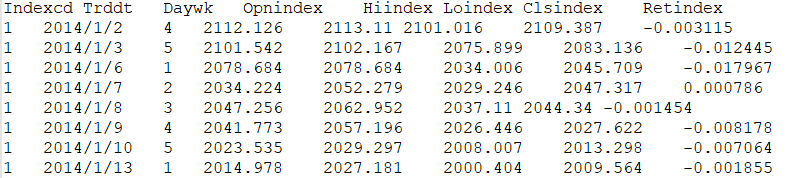
\includegraphics[height=3cm]{images/f000001}
\end{figure}
其运行结果为:
\begin{figure}[H]
	\caption{运行结果}
	\label{f000002}
	\centering
	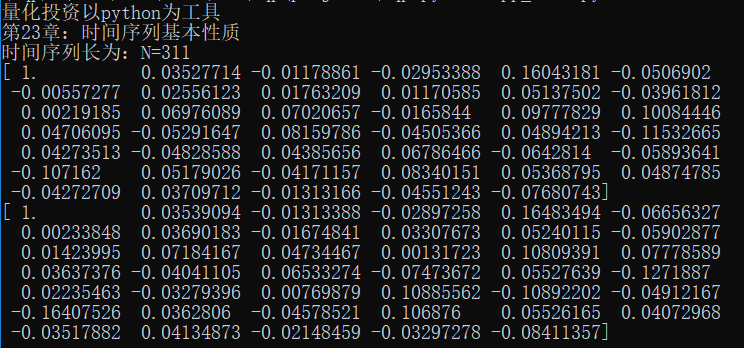
\includegraphics[height=3cm]{images/f000002}
\end{figure}
在图\ref{f000002}中,第一个数据为自相关系数函数ACF各期的值,而第二个数组为偏自相关系数函数PACF各期的值。判断时间序列是否具有自相关性,可以看除ACF和PACF中,除第一个元素外,有没有显著超过阈值的元素,阈值定义为:
\begin{equation}
threshold=\frac{1.96}{\sqrt{N}} = \frac{1.96}{\sqrt{311}} = 0.11
\label{e000017}
\end{equation}
式\ref{e000017}中的N为时间序列样本数,在本例中,共有311条记录,故N=311,所以其阈值为0.11左右。由于$acf[4]=0.16>0.11$所以可以推断其具有自相关性,同时$pacf[4]=0.165>0.11$也可以推断其具有自相关性。我们还可以通过图形的方式形像的表示出来,自相关系数函数图如所示:
\begin{figure}[H]
	\caption{自相关系数函数图}
	\label{f000003}
	\centering
	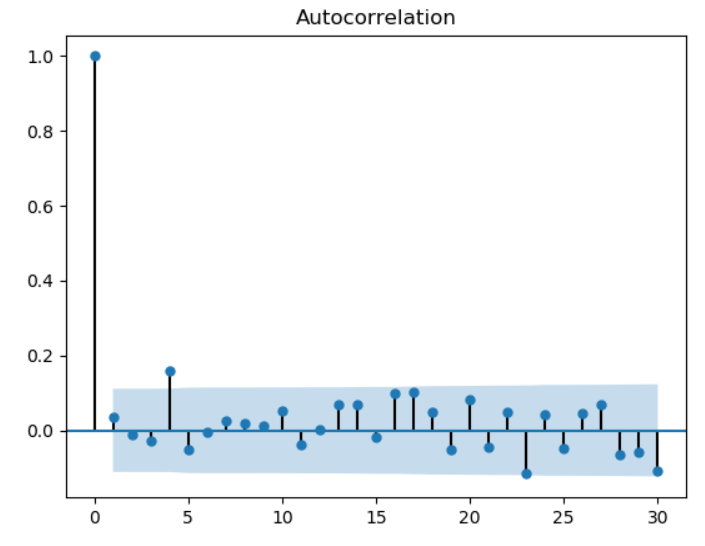
\includegraphics[height=4cm]{images/f000003}
\end{figure}
图\ref{f000003}中蓝色区域的界限为$[-\frac{1.96}{\sqrt{N}}, \frac{1.96}{\sqrt{N}}]=[-0.11, 0.11]$,除第1项外,其他项如果超出蓝色区域则说明此时间序列具有自相关性。\newline
偏自相关系数函数图为:
\begin{figure}[H]
	\caption{偏自相关系数函数图}
	\label{f000004}
	\centering
	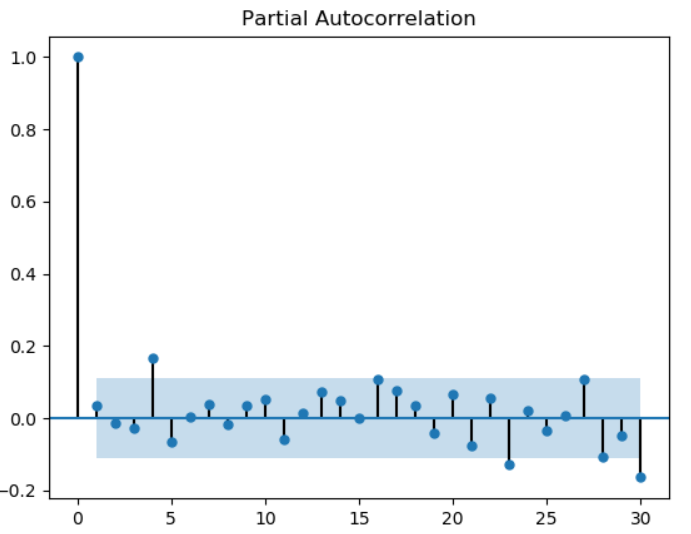
\includegraphics[height=4cm]{images/f000004}
\end{figure}
\subsection{白噪声和随机游走}
\subsubsection{残差序列定义}
我们要对任意时间序列$y_{t}$进行建模,我们的模型为$\hat{y}_{t}$,残差序列$x_{t}$可以定义为:$x_{t}=y_{t}-\hat{y}_{t}$,我们的任务就是使残差时间序列中每一个时间点对应的随机变量互相独立,没有自相关性,即满足独立同分布(Independent and Identical Distribution,I.I.D)条件。如果各个随机变量$x_{t} \sim \mathbb{N}(0, \sigma ^{2})$,则称其为高斯白噪声。\newline
\subsubsection{差分运算符}
为了后续讨论问题方便,我们首先定义BSO运算符:
\begin{equation}
Bx_{t}=x_{t-1} \quad B^{n}x_{t}=x_{t-n}
\label{e000018}
\end{equation}
我们定义差分运算符为:
\begin{equation}
\begin{aligned}
\nabla x_{t} = x_{t}-x_{t-1}=(1-B)x_{t} \\
\nabla x_{t}^{n} = \big( x_{t}-x_{t-n} \big)^{n}=(1-B)^{n}x_{t}
\end{aligned}
\label{e000019}
\end{equation}
\subsubsection{白噪声定义}
对于时间序列$\{ w_{t}, t=1,2,3,...,N \}$,满足$\forall t \quad w_{t} \sim \mathcal{N}(0, \sigma ^{2})$且$\forall i \ne j \quad Cor(w_{i}, w_{j})=0$,则其为白噪声时间序列。\newline
下面我们来看白噪声的二阶属性:
\begin{equation}
\begin{aligned}
\mu = E(w_{t})=0 \\
\gamma _{k}= Cor(w_{t}, w_{t+k}) = \begin{cases}
1 \quad if \quad k=0 \\
0 \quad if \quad k \ne 0
\end{cases}
\end{aligned}
\label{e000020}
\end{equation}
\subsubsection{随机游走}
随机游走(Random Walk)时间序列是指$x_{t}$可以定义为:$x_{t}=x_{t-1}+w_{t}$,其中$w_{t}$为白噪声时间序列。随机游走时间序列可以表示为:
\begin{equation}
\begin{aligned}
x_{t}=x_{t-1}+w_{t}=Bx_{t}+w_{t} \\
x_{t}=x_{t-1}+w_{t}=x_{t-2}+w_{t-1}+w_{t} \\
...... \\
x_{t}=w_{1} + w_{2} + ... + w_{t-1} + w_{t}
\end{aligned}
\label{e000021}
\end{equation}
所以随机游走时间序列可以看作是多个白噪声时间序列的叠加。下面我们来看随机游走时间序列的均值和协方差:
\begin{equation}
\begin{aligned}
\mu = 0 \\
\gamma _{k}(t)=Cov(x_{t}, x_{t+k})=t \sigma ^{2}
\end{aligned}
\label{e000022}
\end{equation}
我们再来看随机游走序列的自相关系数函数ACF:
\begin{equation}
\begin{aligned}
\rho _{k}(t)=\frac{Cov(x_{t}, x_{t+k})}{\sqrt{ Var(x_{t}) \cdot Var(x_{t+k}) }} \\
=\frac{t \sigma ^{2}}{\sqrt{t \sigma ^{2} (t+k) \sigma ^{2}}}=\frac{1}{\sqrt{1+ \frac{k}{t} }}
\end{aligned}
\label{e000023}
\end{equation}
在通常情况下,t比k要大得多,因此$\rho_{k}$会比较接近于1。\newline
下面我们来模拟一个随机游走时间序列信号,程序如下所示:
\lstset{language=PYTHON, caption={随机游走过程模拟}, label={c000003}}
\begin{lstlisting}
    def random_wale_demo(self):
        '''
        随机游走时间序列建模示例
        '''
        w = np.random.standard_normal(size=1000)
        x = w
        for t in range(1, len(w)):
            x[t] = x[t-1] + w[t]
        plt.plot(x, c='b')
        plt.title('Random Walk Demo')
        plt.show()
        acfs = stattools.acf(x)
        print(acfs)
        tsaplots.plot_acf(x, use_vlines=True, lags=30)
        plt.show()
        # 拟合随机游走信号
        r = []
        for t in range(1, len(x)):
            r.append(x[t] - x[t-1])
        rd = np.array(r)
        plt.plot(rd, c='r')
        plt.title('Residue Signal')
        plt.show()
        rd_acfs = stattools.acf(rd)
        print(rd_acfs)
        tsaplots.plot_acf(rd, use_vlines=True, lags=30)
        plt.show()
\end{lstlisting}
我们首先通过$x_{t}=x_{t-1}+w_{t}$生成一个随机游走信号,该信号图形如下所示:
\begin{figure}[H]
	\caption{随机游走时间序列信号}
	\label{f000005}
	\centering
	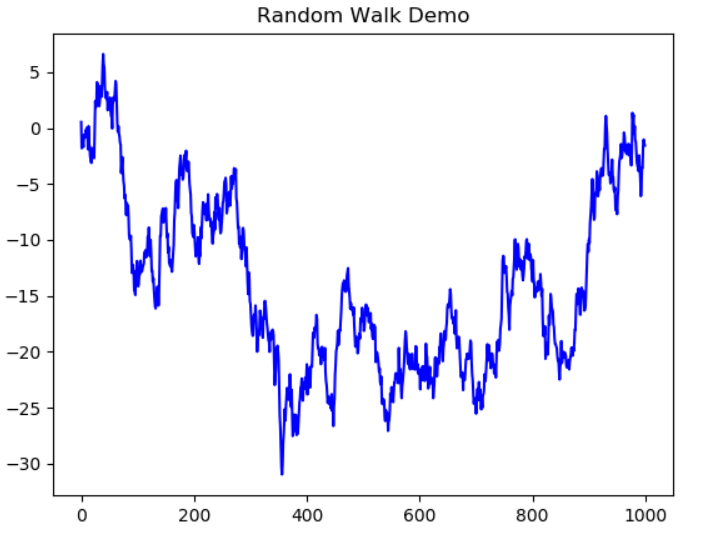
\includegraphics[height=5cm]{images/f000005}
\end{figure}
由图\ref{f000005}可以看出,其非常像是一个股票收盘价的走势图,这也是为什么有些人说股票走势是随机游走过程了。接着我们求出该时间序列的自相关系数函数ACF及其自相关图,如下所示:
\begin{figure}[H]
	\caption{随机游走时间序列信号}
	\label{f000006}
	\centering
	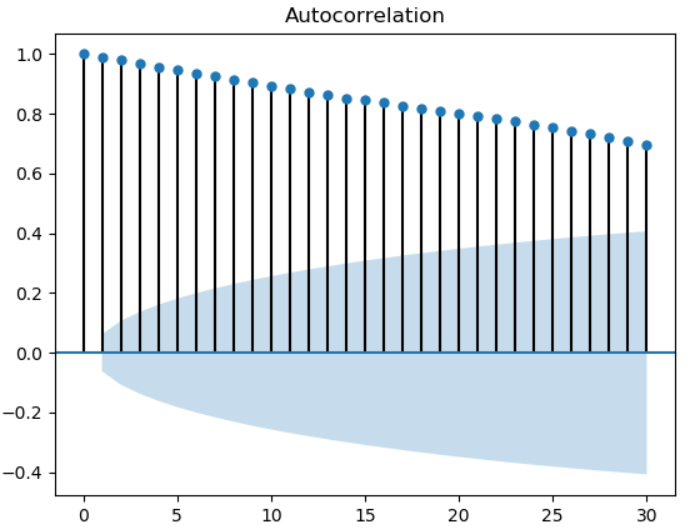
\includegraphics[height=5cm]{images/f000006}
\end{figure}
由图可以看出,其具有极强的自相关性,所有ACF值均位于蓝色置信区间之外。\newline
我们知道$x_{t}-x_{t-1}=w_t$,而$w_t$是白噪声时间序列信号,这实际上模拟了实际应用过程,我们把$x_t$视为实际的金融信号,而$x_{t-1}$为我们建模的信号,将两个信号相减,得到残差信号,如果残差信号是白噪声信号,就可以认为我们建模是合理的。下面来看我们得到的残差信号:
\begin{figure}[H]
	\caption{残差时间序列信号}
	\label{f000007}
	\centering
	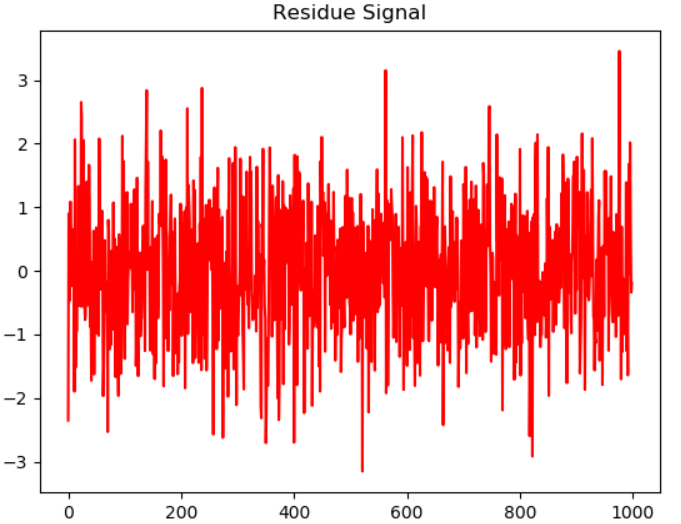
\includegraphics[height=5cm]{images/f000007}
\end{figure}
计算并绘制ACF如下所示:
\begin{figure}[H]
	\caption{残差自相关系数函数}
	\label{f000008}
	\centering
	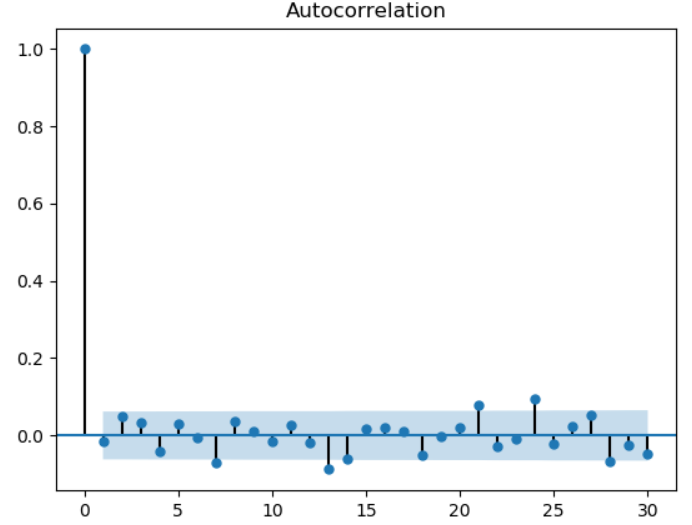
\includegraphics[height=5cm]{images/f000008}
\end{figure}
程序的运行结果如下所示:
\begin{figure}[H]
	\caption{程序运行结果}
	\label{f000009}
	\centering
	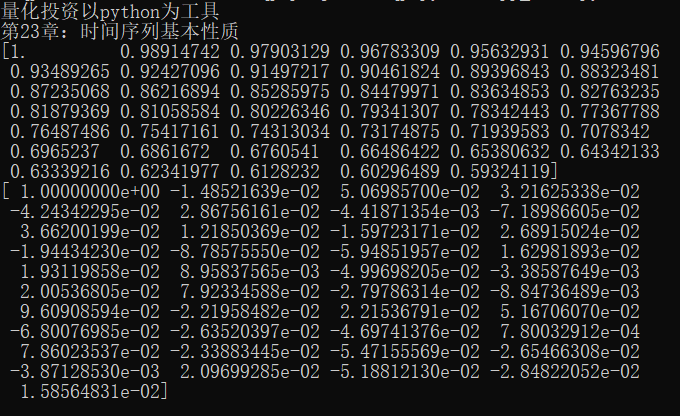
\includegraphics[height=5cm]{images/f000009}
\end{figure}
下面我们以上证综指收益率为例,来看随机游走模型是否可以很好的拟合这个时间序列,程序如下所示:
\lstset{language=PYTHON, caption={随机游走拟合上证综指收益率}, label={c000004}}
\begin{lstlisting}
    def random_walk_fit(self):
        data = pd.read_csv(self.data_file, sep='\t', index_col='Trddt')
        sh_index = data[data.Indexcd==1]
        sh_index.index = pd.to_datetime(sh_index.index)
        sh_return = sh_index.Retindex
        print('时间序列长为:N={0}'.format(len(sh_return)))
        r = []
        for t in range(1, len(sh_return)):
            r.append(sh_return[t] - sh_return[t-1])
        rd = np.array(r)
        plt.plot(rd, c='b')
        plt.title('Random Walk fit SHIndex Return')
        plt.show()
        rd_acfs = stattools.acf(rd)
        print(rd_acfs)
        tsaplots.plot_acf(rd, use_vlines=True, lags=30)
        plt.show()
\end{lstlisting}
其残差图像为:
\begin{figure}[H]
	\caption{残差图形}
	\label{f000010}
	\centering
	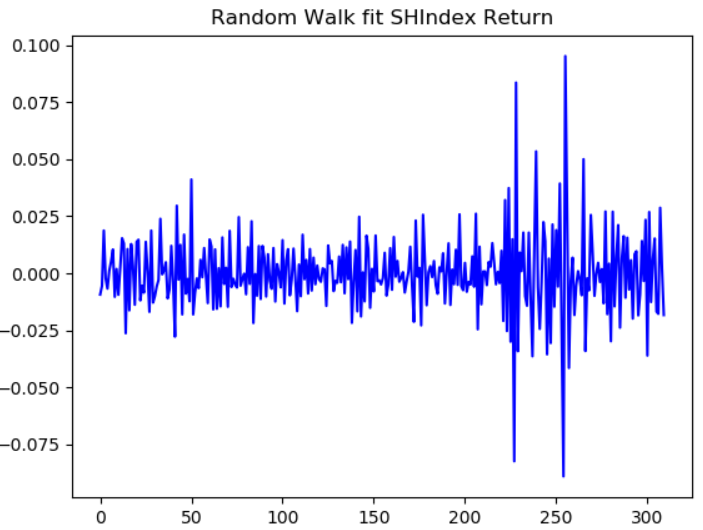
\includegraphics[height=5cm]{images/f000010}
\end{figure}
自相关系数函数ACF图形:
\begin{figure}[H]
	\caption{自相关系数函数ACF}
	\label{f000011}
	\centering
	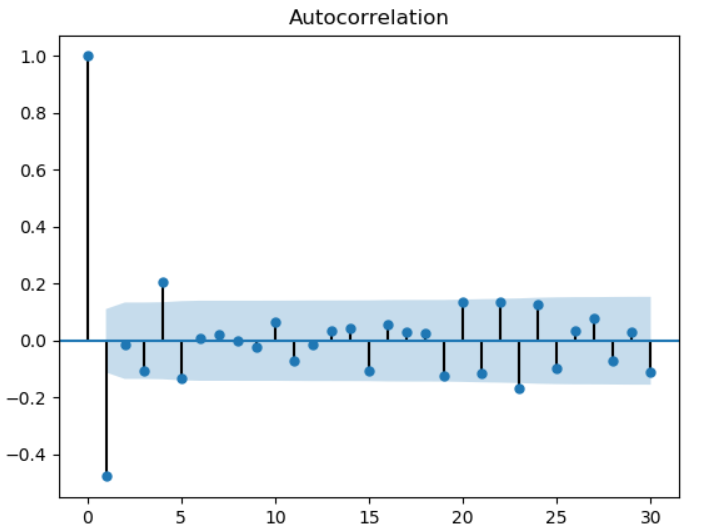
\includegraphics[height=5cm]{images/f000011}
\end{figure}
由图\ref{f000011}所示,在1、4时间点,明显超出置信范围,因此随机游走过程不能很好的拟合上证综指收益率时间序列信号。程序的运行结果如下所示:
\begin{figure}[H]
	\caption{程序运行结果}
	\label{f000012}
	\centering
	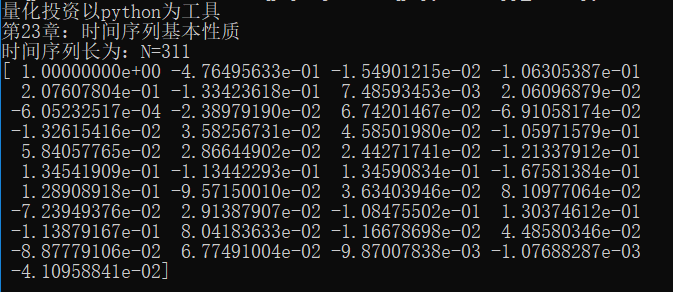
\includegraphics[height=5cm]{images/f000012}
\end{figure}

\maketitle\begin{center}
\Large \textbf{第2章 ARIMA模型}
\end{center}
\begin{abstract}
在本章中我们将首先讲述自回归模型AR(p),接着讲述移动平均MA(q),最后讲解ARMA(p,q),然后将其泛化为ARIMA(p,d,q),
分别将这些模型用于实际金融时间序列数据拟合。aqt001.py
\end{abstract}
\section{ARIMA模型}
\subsection{稳定性和模型选择标准}
\subsubsection{强稳定性}
在我们以前的讨论中,我们说如果一个时间序列各个时间点所对应的随机变量,只要均值和方差不变,就是平稳时间序列。下面我们对强平稳性进行定义。\newline
对于一个时间序列$\{ x_{t} \}$,如果对于$\forall t_{i},m$,两个序列:$x_{t_1}, x_{t_2},...,x_{t_N}$和$x_{t_1+m}, x_{t_2+m},...,x_{t_N+m}$的统计特性完全相同,则说明该时间序列为强平稳特性。
\subsubsection{模型选择标准}
我们将用AIC来进行模型选择,AIC的全称为:Akaike Information Criterion,我们通常会选择AIC值较小的模型。在实际应用中,还可以使用BIC来进行模型选择,BIC的全称为Bayes Information Criterion。在本章中我们只用AIC来进行模型选择。\newline
假设统计模型的似然函数有$k$参数,最大似然值为$L$,则AIC定义为:
\begin{equation}
AIC=-2\log(L) + 2k
\label{e000024}
\end{equation}
由式\ref{e000024}可知,最大似然值越大或者参数越少,AIC的值越小,模型就越是好模型。
\subsubsection{ADF检验}
在前面所讨论的问题中,我们通常根据自相关系数函数ACF和偏自相关系数函数PACF来判断稳定性,但是主观性比较强,我们需要一个客观的标准。\newline
我们首先来定义时间序列的阶数,对于下面的非平稳时间序列:
\begin{equation}
x_{t}=x_{t-1}+w_{t}
\label{e000036}
\end{equation}
其中$w_{t} \sim \mathcal{N}(0, \sigma ^{2})$为白噪声信号,且$x_{0}=0$,我们可以得到其均值为:
\begin{equation}
E(x_{t})=E(x_{t-1}+w_{t})=E(x_{t-1})+E(w_{t})=E(x_{t-1})=...=E(x_{0})=0
\label{e000037}
\end{equation}
同样我们可以得到其方差:
\begin{equation}
Var(x_{t})=Var(x_{t-1}+w_{t})=Var(x_{t-1})+Var(w_{t})=Var(x_{t-1})+\sigma ^{2}=...=t\sigma ^{2}
\label{e000038}
\end{equation}
$x_{t}$由于其各时间点对应的随机变量的方差随时间变化,因此不是平稳时间序列。\newline
我们定义1阶差分算子:
\begin{equation}
\nabla x_{t} = Bx_{t}=x_{t}-x_{t-1}=w_{t}
\label{e000039}
\end{equation}
对于$Bx_{t}$为白噪声信号,其显然是平稳时间序列,所以我们称$x_{t}$为I(1)的非平稳时间序列。我们可以将其定义扩展到$n$阶:
\begin{equation}
Bx_{t}=x_{t-1} \quad B^{2}x_{t}=x_{t-2} \quad B^{3}x_{t}=x_{t-3} \quad ...  \quad B^{n}x_{t}=x_{t-n}
\label{e000040}
\end{equation}
我们还以上面的时间序列$x_{t}=x_{t-1}+w_t$为例,我们可以将其写为:
\begin{equation}
x_{t}-x_{t-1}=x_{t}-Bx_{t}=(1-B)x_{t}=w_{t}
\label{e000041}
\end{equation}
式\ref{e000041}中$1-B$为滞后算子多项式,我们令$1-B=0$得出的解为$B=1$,其为单位根,所以其为非平稳时间序列。这一结论可以推广到更一般的情况,对于如下所示的时间序列:
\begin{equation}
y_{t}=(1+\rho)y_{t-1}-\rho y_{t-2}+w_{t}
\label{e000042}
\end{equation}
其所对应的滞后算子多项式为:
\begin{equation}
y_{t}-(1-\rho)By_{t}+\rho B^{2} y_{t}=w_{t}
\label{e000043}
\end{equation}
令式\ref{e000043}左边为0,得到的解为:$B=1$和$B=\frac{1}{\rho}$,因为其存在单位根,所以其不是平稳时间序列。\newline
对于任意如下所示时间序列:
\begin{equation}
y_{t}=\gamma + \rho _{1}y_{t-1} + \rho _{2}y_{t-2} + ... + \rho _{p}y_{t-p} + w_{t}
\label{e000044}
\end{equation}
其中$w_{t} \sim \mathcal{N}(0, \sigma ^{2})$为独立同分布(i.i.d)噪声信号。
可以将式\ref{e000044}改写为如下形式:
\begin{equation}
y_{t}=\gamma + \rho _{1}By_{t} + \rho _{2}B^{2}y_{t} + ...  + \rho _{p}B^{p}y_{t} + w_{t}
\label{e000045}
\end{equation}
将式\ref{e000045}右边所有包含$y_{t}$的项都移到左边,可以得到下式:
\begin{equation}
(1-\rho _{1}B - \rho _{2}B^{2} - .. - \rho _{p}B^{p})y_{t}=\gamma + w_{t}
\label{e000046}
\end{equation}
可以得到其对应的滞后算子多项式方程为:
\begin{equation}
1-\rho(B)=1-\rho _{1}B - \rho _{2}B^{2} - .. - \rho _{p}B^{p}=0
\label{e000047}
\end{equation}
解这个方程,如果所有解的绝对值均大于1,则该时间序列为平稳时间序列,如果存在单位根或绝对值小于1的根,则其为非平稳时间序列。\newline
以上我们讲解的判断时间序列平稳性的原理,在实际应用中,我们通常采用ADF来判断时间序列的平稳性,ADF模型如下所示:
\begin{equation}
\Delta y_{t}=\alpha + \beta t + \gamma y_{t-1} + \delta _{1}\Delta y_{t-1} + \delta _{2}\Delta y_{t-2} + ... + \delta _{p}\Delta y_{t-p} + w_{t}
\label{e000048}
\end{equation}
其中$\alpha$对应截距,$\beta$对应趋势,$\delta _{1}\Delta y_{t-1} + \delta _{2}\Delta y_{t-2} + ... + \delta _{p}\Delta y_{t-p}$为ADF的增广项,p为增广项的期数,其值由AIC或BIC算法来决定。原假设$H_{0}$为该序列有单位根是非平稳时间序列:$\gamma = 0$;备择假设$H_{1}$为该序列为平稳时间序列:$\gamma < 0$。\newline
这部分原理比较复杂,我们在实际应用中,通常使用arch包中的ADF函数来完成检验工作,其函数定义为:
\begin{equation}
ADF(y, lags, trend, max_lags, method)
\label{e000049}
\end{equation}
其中:
\begin{itemize}
\item y:待判断的时间序列;
\item lags:滞后期数
\item trend:用来控制检验模型的类型
	\begin{itemize}
	\item 'nc':不含截距项;
	\item 'c':含截距项;
	\item 'ct':包含截距项和线性趋势项;
	\item 'ctt':包含截距项和线性趋势项以及二次趋势项;
	\end{itemize}
\item max\_lags:最大期数
\item method:常用方法为:'aic'、 'bic'、 't\_stat'
\end{itemize}
下面我们通过一个例子来看怎样使用ADF方法,我们以上证综指收益率和收盘价这两个序列为例,我们首先需要安装python的garch库:
\lstset{language=BASH}
\begin{lstlisting}
pip install arch
\end{lstlisting}
程序代码如下所示:
\lstset{language=PYTHON, caption={ADF检验}, label={c000006}}
\begin{lstlisting}
import arch.unitroot as unitroot
......
    def adf_demo(self):
        print('ADF检验例程...')
        data = pd.read_csv(self.data_file, sep='\t', index_col='Trddt')
        sh_index = data[data.Indexcd==1]
        sh_index.index = pd.to_datetime(sh_index.index)
        sh_return = sh_index.Retindex
        sh_return_adf = unitroot.ADF(sh_return)
        print(sh_return_adf.summary().as_text())
        print('stat={0:0.4f}; pvalue={0:0.4f}'.format(sh_return_adf.stat, sh_return_adf.pvalue))
        print('critical_values:{0}'.format(sh_return_adf.critical_values))
        print('1%value={0}'.format(sh_return_adf.critical_values['1%']))
        if sh_return_adf.stat < sh_return_adf.critical_values['1%']:
            print('上证综指收益率为平稳时间序列 ^_^')
        else:
            print('上证综指收益率为平稳时间序列  !!!!!!!!!')
        sh_close = sh_index.Clsindex
        sh_close_adf = unitroot.ADF(sh_close)
        if sh_close_adf.stat < sh_close_adf.critical_values['1%']:
            print('上证综指收盘价为平稳时间序列 ^_^')
        else:
            print('上证综指收盘价为非平稳时间序列 !!!!!!!')
\end{lstlisting}
运行结果如下所示:
\begin{figure}[H]
	\caption{自相关系数函数ACF}
	\label{f000022}
	\centering
	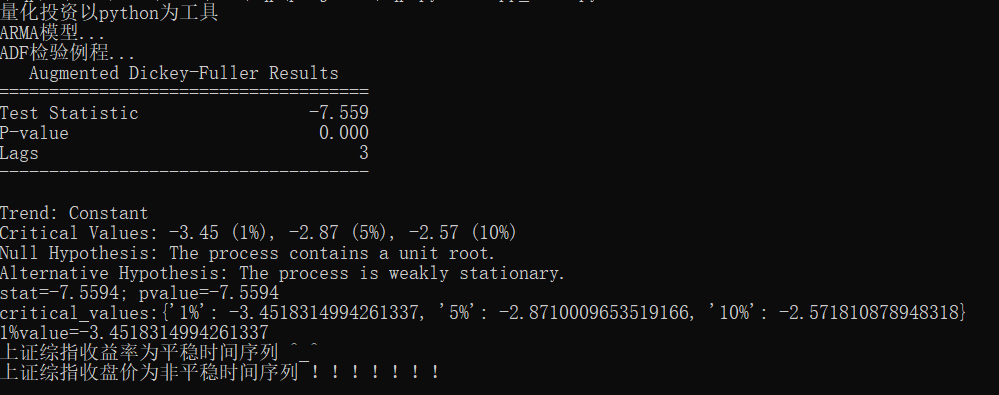
\includegraphics[height=5cm]{images/f000022}
\end{figure}
由上面的结果可以看出,上证综指收益率是稳定的时间序列,收盘价却是不稳定的时间序列。
\subsection{自回归模型}
\subsubsection{背景}
我们可以扩展随机游走模型,使当前时间点数据不仅依赖前一时间点的值,同时还依赖前p个时间点的值,是这p个值的线性组合,
这就得到了自回归模型。
\subsubsection{模型定义}
自回归模型AR(p)是随机游走模型的扩展,p阶自回归模型定义为:
\begin{equation}
x_{t}=\alpha _{1}x_{t-1} + \alpha _{2}x_{t-2} + ... + \alpha _{p}x_{t-p} + w_{t} = \sum_{i=1}^{p} \alpha _{i}x_{t-i} + w_{t}
\label{e000025}
\end{equation}
其中$\{ w_{t} \}$为白噪声,$\alpha _{i} \in R$且$\alpha_{p} \ne 0$。\newline
当$p=1$且$\alpha _{1}=1$时,自回归模型就退化为随机游走模型。\newline
为后续讨论方便,我们定义如下运算符:
\begin{equation}
\theta _{p}(B)x_{t}=(1-\alpha _{1}B-\alpha _{2}B^{2}-...-\alpha _{p}B^{p})x_{t}=w_{t}
\label{e000026}
\end{equation}
有了上述模型之后,我们就可以直接拿来作预测,如下所示:
\begin{equation}
\begin{aligned}
    \hat{x}_t=\alpha _{1}x_{t-1}+\alpha _{2}x_{t-2}+...+\alpha _{p}x_{t-p} \\
    \hat{x}_{t+1}=\alpha _{1}\hat{x}_{t}+\alpha _{2}x_{t-1}+...+\alpha _{p}x_{t-p+1}
\end{aligned}
\label{e000027}
\end{equation}
然后依此类推,可以求出其后n个时间点的预测值。
\subsubsection{二阶特性}
我们首先定义特性方程:
\begin{equation}
\theta _{p}(B)=0
\label{e000028}
\end{equation}
解这个方程得到的解的绝对值必须大于才是平稳序列。我们可以举几个实例,首先是随机游走序列:
\paragraph{随机游走}
根据定义$x_{t}=x_{t-1}+w_{t}$我们可以得到$\alpha _1=1$,其特性方程为$\theta=1-B=0$,其解为$B=1$,因为其解的
绝对值不大于1,所以其不是平稳模型。
\paragraph{1阶自回归}
我们假设自回归模型为$x_{t}=\frac{1}{4}x_{t-1}+w_{t}$,其中$\alpha _1=\frac{1}{4}$,
其特性方程为$\theta = 1-\frac{1}{4}=0$,其解为$B=4$,该解绝对值大于1,所以其是平稳模型。
\paragraph{2阶自回归模型}
我们假设自回归模型为$x_{t}=\frac{1}{2}x_{t-1}+\frac{1}{2}x_{t-2}+w_{t}$,其特性方程为
$\theta _2(B)=\frac{1}{2}(1-B)(B+2)=0$,则其解为$B=1,-2$,其中一个解为单位根,其绝对值不大于1,因此本模型不是
平稳模型。虽然本模型不是平稳模型,但是其他2阶自回归模型是完全有可能是平稳模型的。
\paragraph{二阶特性}
均值、自协方差、自相关系数定义如下所示:
\begin{equation}
\begin{aligned}
\mu _{x}=E(x_{t})=0 \\
\gamma _{k}=\sum_{i=1}^{p}\alpha _{i} \gamma _{k-i}, \quad k>0 \\
\rho _{k} = \sum_{i=1}^{p}\alpha _{i} \rho _{k-i}, \quad k>0
\end{aligned}
\label{e000029}
\end{equation}
\subsubsection{模拟数据}
下面我们来模拟一个AR(2)的时间序列,我们的数据生成和拟合代码如下所示:
\lstset{language=PYTHON, caption={AR数据模拟和拟合示例}, label={c000004}}
\begin{lstlisting}
import numpy as np
import pandas as pd
import matplotlib.pyplot as plt
import matplotlib.dates as mdates
from matplotlib.font_manager import FontProperties
from statsmodels.tsa import stattools
from statsmodels.graphics import tsaplots
from statsmodels.tsa.arima_model import ARIMA

class Aqt001(object):
    def __init__(self):
        self.name = 'Aqt001'
        
    def startup(self):
        print('ARMA模型...')
        self.simulate_ar2()
        
    def simulate_ar2(self):
        print('模拟AR(2)')
        alpha1 = 0.666
        alpha2 = -0.333
        wt = np.random.standard_normal(size=1000)
        x = wt
        for t in range(2, len(wt)):
            x[t] = alpha1 * x[t-1] + alpha2 * x[t-2] + wt[t]
        plt.plot(x, c='b')
        plt.show()
        ar2 = stattools.ARMA(x, (2, 0)).fit(disp=False)
        print('p={0} **** {1}; q={2}***{3}; {4} - {5} - {6}'.format(
                    ar2.k_ar, ar2.arparams, ar2.k_ma, ar2.maparams, 
                    ar2.aic, ar2.bic, ar2.hqic)
        )
        arima2_0_0 = ARIMA(x, order=(2, 0, 0)).fit(disp=False)
        print('ARIMA: p={0} **** {1}; q={2}***{3}; {4} - {5} - {6}'. \
                    format(arima2_0_0.k_ar, arima2_0_0.arparams, 
                    arima2_0_0.k_ma, arima2_0_0.maparams, 
                    arima2_0_0.aic, arima2_0_0.bic, 
                    arima2_0_0.hqic)
        )
        resid = arima2_0_0.resid
        # 绘制ACF
        acfs = stattools.acf(resid)
        print(acfs)
        tsaplots.plot_acf(resid, use_vlines=True, lags=30)
        plt.title('ACF figure')
        plt.show()
        pacfs = stattools.pacf(resid)
        print(pacfs)
        tsaplots.plot_pacf(resid, use_vlines=True, lags=30)
        plt.title('PACF figure')
        plt.show()
\end{lstlisting}
我们首先生成一个1000个数据点的均值为0方差为1的白噪声数据,然后根据$x_{t}=\alpha _{1}x_{t-1} + \alpha _{2}x_{t-2} + w_{t}=0.666 \times x_{t-1} - 0.333 \times x_{t-2} + w_{t}$公式,生成拟合数据。我们绘制该模拟数据图像,接着我们分别用ARMA和ARIMA进行拟合,求出系数,然后计算出模拟选择的参数:AIC、BIC、HQIC的值,最后我们求出模型拟合的残差,并绘制出残差自相关系数函数ACF和偏自相关系数函数PACF的图像。
模拟数据图像为:
\begin{figure}[H]
	\caption{AR2模拟生成数据图}
	\label{f000013}
	\centering
	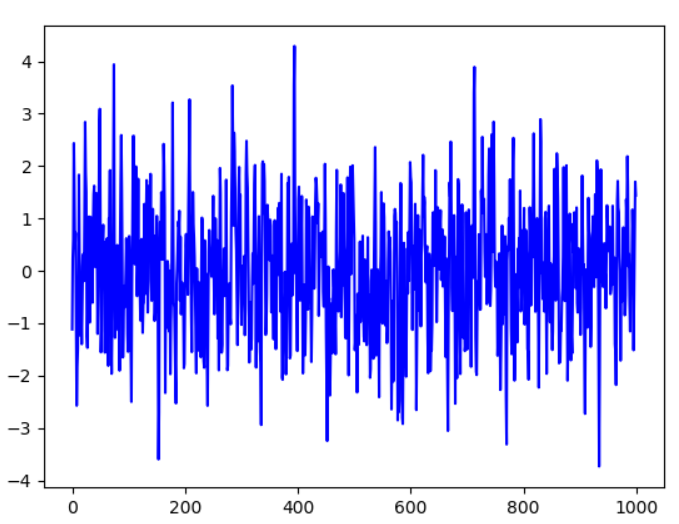
\includegraphics[height=5cm]{images/f000013}
\end{figure}
无论是ARMA还是ARIMA拟合,我们都可以得到较为正确的数据,同时残差的ACF和PACF也表明其是白噪声序列,运行结果如下所示:
\begin{figure}[H]
	\caption{程序运行结果}
	\label{f000014}
	\centering
	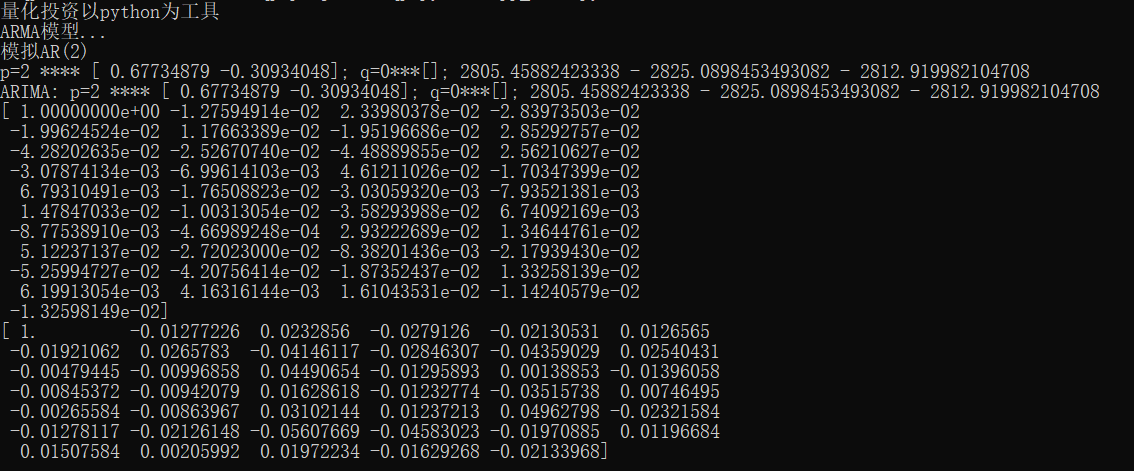
\includegraphics[height=5cm]{images/f000014}
\end{figure}
残差的自相关系数函数ACF图:
\begin{figure}[H]
	\caption{残差的自相关系数函数ACF图}
	\label{f000015}
	\centering
	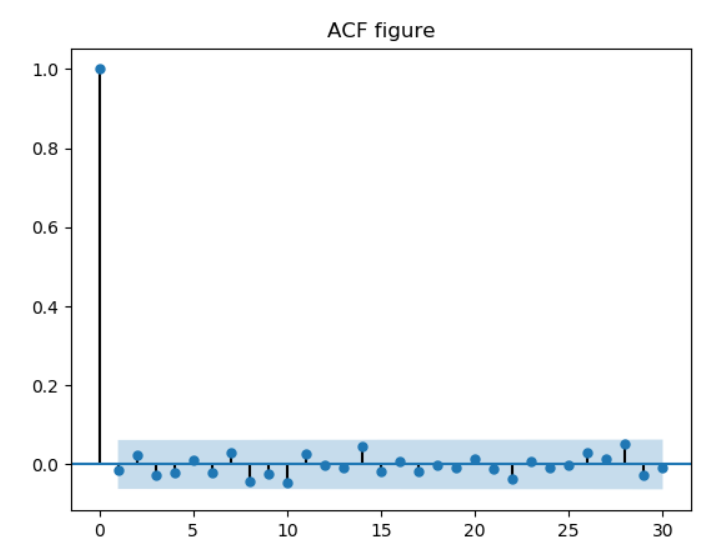
\includegraphics[height=5cm]{images/f000015}
\end{figure}
残差的偏自相关系数函数PACF图:
\begin{figure}[H]
	\caption{残差的偏自相关系数函数PACF图}
	\label{f000016}
	\centering
	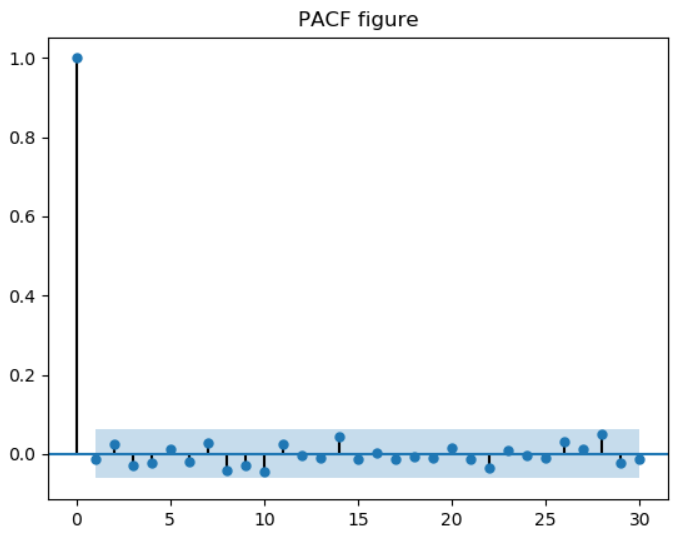
\includegraphics[height=5cm]{images/f000016}
\end{figure}
由ACF和PACF图可以看出,我们残差是比较典型的随机白噪声序列,由此可见我们拟合还是很好的。
\subsubsection{展望}
在理解了基本理论之后,我们将引入最终的ARIMA模型,并用ARIMA模型来拟合真实上证综指收盘价时间序列,并用我们的拟合模型来预测最后5日的收盘价,在这个实际例子中,看我们模型的表现如何。
\subsection{ARIMA模型}
\subsubsection{背景}
我们不仅可以对当前时间点数值对之前时间点数值进行建模,我们也可以对前面时间点随机噪声对当前时间点的影响进行建模,同时由于原始信号可能非常不平稳,但是我们求出其差值序列后,可能就变为平稳序列了,这就是ARIMA模型要解决的问题。为了讨论ARIMA模型,我们首先介绍差分的概念:
\begin{equation}
\begin{aligned}
\{ x_1,x_2,...,x_N \} \\
\{d_1^{1},d_2^{1},...,d_{N-1}^{1}\}=\{x_2-x_1,x_3-x_2,...,x_{N}-x_{N-1}\} \\
\{d_1^{2},d_2^{2},...,d_{N-1}^{2}\}=\{d_2^{1}-d_1^{1},d_3^{1}-d_2^{1},...,d_{N-1}^{1}-d_{N-1}^{1}\}
\end{aligned}
\label{e000030}
\end{equation}
上式中分别为原始时序信号,然后是一阶差分和二阶差分。
\subsubsection{模型选择标准}
\paragraph{BIC定义}
我们已经介绍过一个模型选择标准AIC(Akaike Information Criterion),其会惩罚参数多的模型,因为这些模型容易产生过拟合(Overfitting)。接下来我们要介绍另一个模型选择参数BIC(Bayes Information Criterion),与AIC相比,其会更倾向于惩罚参数多的模型,同样是值越小越好,BIC定义如下所示:
\begin{equation}
BIC=-2\log (L) + k \log N
\label{e000031}
\end{equation}
其中L为似然函数的最大值,k为模型的参数,N为数据点个数。
\paragraph{Ljung-Box检测}
我们的缺省假设$H_{0}$为:对于一个拟合的时序信号,对所有滞后时点lags,都是独立同分布(i.i.d)的,即不存在相关性。\newline
备择假设$H_{a}$为:这些信号不是独立同分布(i.i.d)的,具有相关性。\newline
我们定义统计量Q:
\begin{equation}
Q=n(n+2)\sum_{k=1}^{h} \frac{\hat{\rho}_{k}^{2}}{n-k}
\label{e000032}
\end{equation}
式\ref{e000032}中$n$为时间序列长度,$h$为最大滞后期数,$\rho _{k}$第$k$自相关系数。Ljung-Box检测原理比较复杂,但是在python语言中,经过运算可以求出Q值,以及大于Q值的概率,实际上我们看1$\sim$12滞后期的Q值和大于Q值的概率,如果该概率小于显著水平如0.05时,就拒绝缺省假设(不存在相关性),选择备择假设,否则反之。
\subsubsection{定义}
同时考虑之前时间点的信号和噪声值,我们就可以得到如下ARMA模型:
\begin{equation}
x_{t}=\alpha _{1}x_{t-1} + \alpha _{2}x_{t-2} + ... + \alpha _{p}x_{t-p} + w_{t} + \beta _1w_{t-1} + \beta _2w_{t-2}+...+ + \beta _{q}w_{t-q}
\label{e000033}
\end{equation}
如果我们对欲研究的信号求出一阶或二阶差分,然后再利用式\ref{e000033}的模型,就是ARIMA模型了。其中$\{ w_{t} \}$为白噪声,其均值为0,方差为$\sigma ^{2}$。\newline
其特性方程可以表示为:
\begin{equation}
\theta _{p}(B)x_{t}=\phi _{q}(B)w_{t}
\label{e000034}
\end{equation}
由上面的讨论可以看出,AR(p)和MA(q)都是ARIMA模型的特殊情况,在同样精度的条件下,ARIMA模型所需参数最小。
\subsubsection{数据仿真}
在理解了ARIMA模型定义之后,我们来模拟一下ARIMA过程。假设我们要模拟的ARIMA模型为:
\begin{equation}
\begin{aligned}
x_{t}=\alpha _{1}x_{t-1} + \alpha _{2}x_{t-2} + w_{t} + \beta _1w_{t-1} + \beta _2w_{t-2} \\
=1.2 \times x_{t-1} - 0.7 \times x_{t-2} + w_{t} - 0.06 \times w_{t-1} - 0.02 \times w_{t-2}
\end{aligned}
\label{e000035}
\end{equation}
生成模拟数据并利用ARIMA拟合的程序如下所示:
\lstset{language=PYTHON, caption={AR数据模拟和拟合示例}, label={c000005}}
\begin{lstlisting}
    def simulate_arima_p_d_q(self):
        print('模拟ARIMA(p,d,q)过程')
        np.random.seed(8)
        alpha1 = 1.2
        alpha2 = -0.7
        beta1 = -0.06
        beta2 = -0.02
        w = np.random.standard_normal(size=1000)
        x = w
        for t in range(2, len(w)):
            x[t] = alpha1 * x[t-1] + alpha2*x[t-2] + w[t] + beta1 * w[t-1] + beta2*w[t-2]
        plt.plot(x, c='b')
        plt.title('ARIMA(p, d, q) Figure')
        plt.show()
        # 查看ACF
        acfs = stattools.acf(x)
        print('ARIMA(q,d,q) ACFS:\r\n{0}'.format(acfs))
        tsaplots.plot_acf(x, use_vlines=True, lags=30)
        plt.title('ARIMA(p,d,q) ACF')
        plt.show()
        # ARIMA拟合
        min_ABQIC = sys.float_info.max
        arima_model = None
        break_loop = False
        '''
        for p in range(0, 5):
            if break_loop:
                break
            for q in range(0, 5):
                print('try {0}, d, {1}...'.format(p, q))
                try:
                    arima_p_d_q = ARIMA(x, order=(p, 0, q)).fit(disp=False)
                    print('..... fit ok')
                    if arima_p_d_q.aic < min_ABQIC:
                        print('..... record good model')
                        min_ABQIC = arima_p_d_q.aic
                        arima_model = arima_p_d_q
                        #if 1==p and 1==q:
                        #    break_loop = True
                except Exception as ex:
                    print('.....!!!!!! Exception')
        print('ARIMA: p={0} **** {1}; q={2}***{3}; {4} - {5} - {6}'. \
                    format(arima_model.k_ar, arima_model.arparams, 
                    arima_model.k_ma, arima_model.maparams, 
                    arima_model.aic, arima_model.bic, 
                    arima_model.hqic)
        )
        '''
        arima_model = ARIMA(x, order=(2, 0, 2)).fit(disp=False)
        print('God_View:ARIMA: p={0} **** {1}; q={2}***{3}; {4} - {5} - {6}'. \
                    format(arima_model.k_ar, arima_model.arparams, 
                    arima_model.k_ma, arima_model.maparams, 
                    arima_model.aic, arima_model.bic, 
                    arima_model.hqic)
        )
        resid = arima_model.resid
        # 绘制ACF
        acfs = stattools.acf(resid)
        print(acfs)
        tsaplots.plot_acf(resid, use_vlines=True, lags=30)
        plt.title('ARIMA(p,d,q) ACF figure')
        plt.show()
        pacfs = stattools.pacf(resid)
        print(pacfs)
        tsaplots.plot_pacf(resid, use_vlines=True, lags=30)
        plt.title('ARIMA(p,d,q) PACF figure')
        plt.show()
\end{lstlisting}
生成的时序信号x为:
\begin{figure}[H]
	\caption{原始模拟信号图}
	\label{f000017}
	\centering
	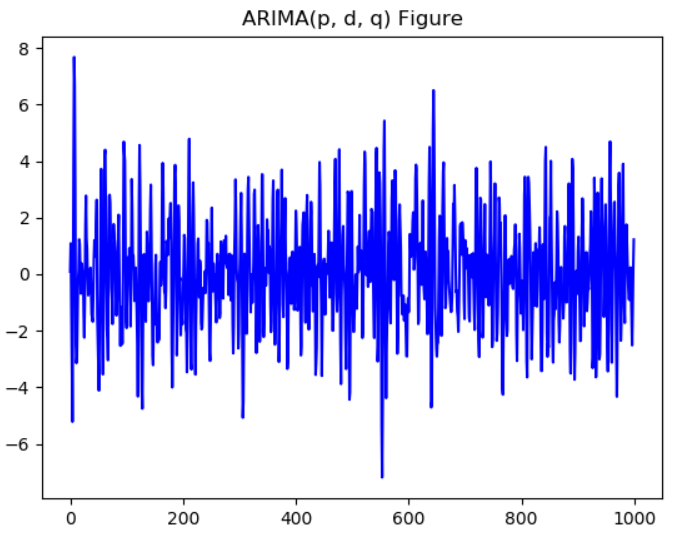
\includegraphics[height=5cm]{images/f000017}
\end{figure}
该信号的自相关系数函数ACF图为:
\begin{figure}[H]
	\caption{原始模拟信号ACF图}
	\label{f000018}
	\centering
	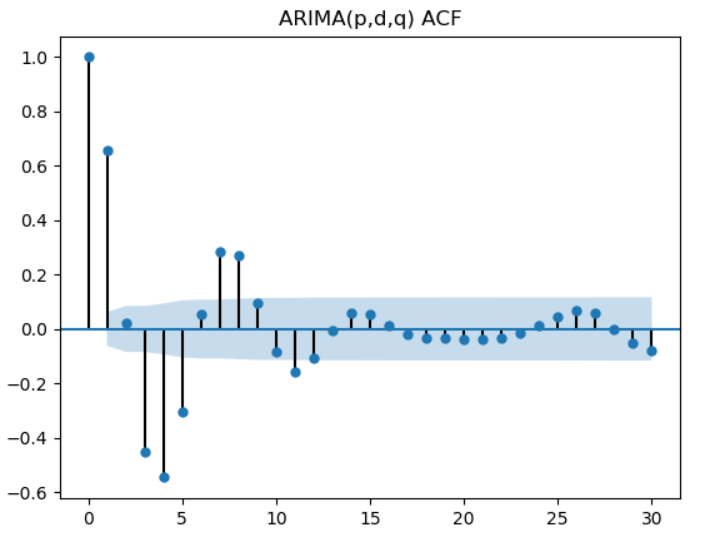
\includegraphics[height=5cm]{images/f000018}
\end{figure}
由图中可以看出,该信号具有非常强的自相关性。\newline
接着我们用ARIMA模型来模拟该信号,上面程序注释部分为求最佳ARIMA模型的p和q参数,以AIC作为模型选择标准,因为我们知道模型为ARIMA(2,0,2),所以我们同时也用ARIMA(2,0,2)来进行拟合,程序运行结果如下所示:
\begin{figure}[H]
	\caption{程序运行结果}
	\label{f000019}
	\centering
	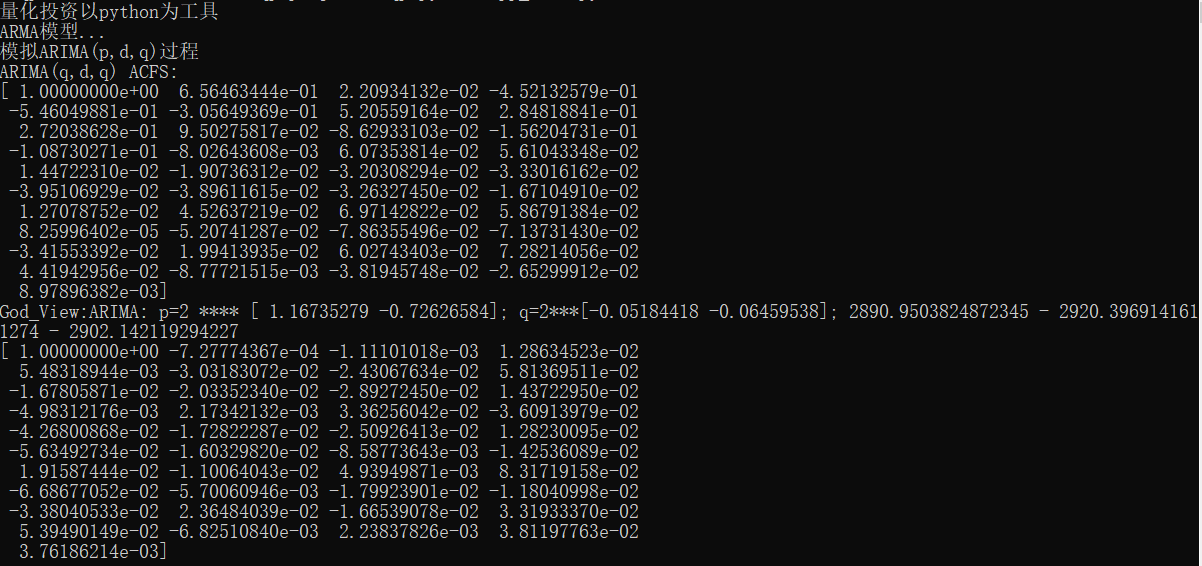
\includegraphics[height=5cm]{images/f000019}
\end{figure}
接着我们求出残差序列,残差序列自相关系数函数ACF图如下所示:
\begin{figure}[H]
	\caption{残差自相关系数函数ACF图}
	\label{f000020}
	\centering
	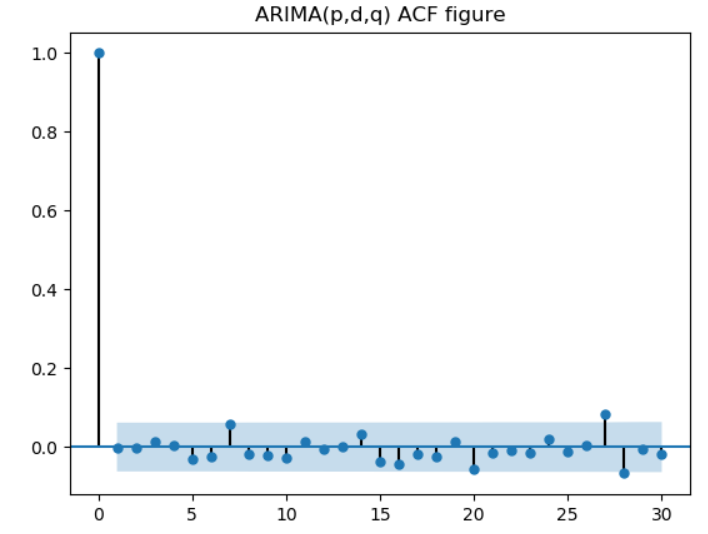
\includegraphics[height=5cm]{images/f000020}
\end{figure}
残差序列偏自相关系数函数图PACF如下所示:
\begin{figure}[H]
	\caption{残差偏自相关系数函数ACF图}
	\label{f000021}
	\centering
	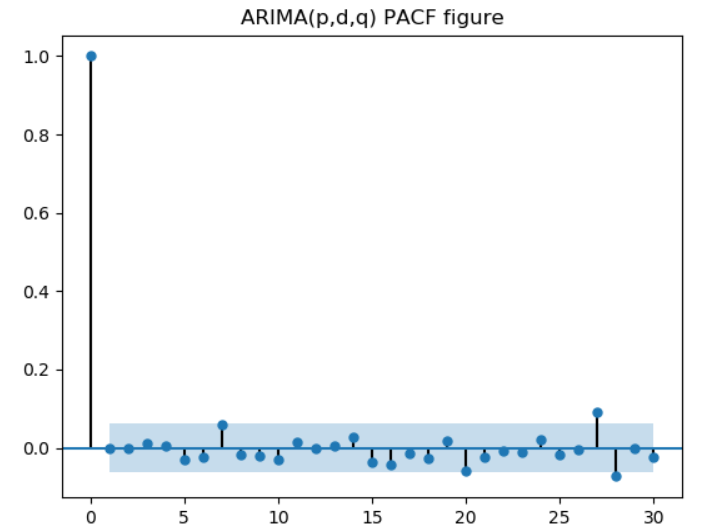
\includegraphics[height=5cm]{images/f000021}
\end{figure}
由图中可以看出,残差序列基本上是白噪声信号。
\subsubsection{金融数据拟合及预测}
接下来我们用ARIMA模型,来拟合上证综指收盘价,我们利用除最后3天的数据来得出ARIMA模型,然后利用拟合出的ARIMA模型来预测后3天的收盘价,来看我们模型的性能。根据经验,对于股票的收盘数据来说,采用取对数后再求1阶差分的形式,可以取得更好的效果,因此我们会先对数据进行预处理,然后再来用ARIMA模型来拟合数据。\newline
程序如下所示:
\lstset{language=PYTHON, caption={ARIMA数据拟合上证综指收盘价}, label={c000007}}
\begin{lstlisting}
    def arima_demo(self):
        register_matplotlib_converters()
        data = pd.read_csv(self.data_file, sep='\t', index_col='Trddt')
        sh_index = data[data.Indexcd==1]
        sh_index.index = pd.to_datetime(sh_index.index)
        raw_data = sh_index.Clsindex
        train_data = raw_data[:-3]
        close_price = np.log(train_data)
        plt.plot(close_price)
        plt.show()
        print(train_data.head(n=3))
        # ARIMA拟合
        min_ABQIC = sys.float_info.max
        arima_model = None
        for p in range(0, 5):
            for q in range(0, 5):
                print('try {0}, d, {1}...'.format(p, q))
                try:
                    arima_p_d_q = ARIMA(close_price, order=(p, 1, q)).fit(disp=False)
                    print('..... fit ok')
                    if arima_p_d_q.aic < min_ABQIC:
                        print('..... record good model')
                        min_ABQIC = arima_p_d_q.aic
                        arima_model = arima_p_d_q
                except Exception as ex:
                    print('.....!!!!!! {0}'.format(ex))
        print('ARIMA: p={0} **** {1}; q={2}***{3}; {4} - {5} - {6}'. \
                    format(arima_model.k_ar, arima_model.arparams, 
                    arima_model.k_ma, arima_model.maparams, 
                    arima_model.aic, arima_model.bic, 
                    arima_model.hqic)
        )
        resid = arima_model.resid
        # 绘制ACF
        acfs = stattools.acf(resid)
        print(acfs)
        tsaplots.plot_acf(resid, use_vlines=True, lags=30)
        plt.title('ARIMA(p,d,q) ACF figure')
        plt.show()
        pacfs = stattools.pacf(resid)
        print(pacfs)
        tsaplots.plot_pacf(resid, use_vlines=True, lags=30)
        plt.title('ARIMA(p,d,q) PACF figure')
        plt.show()
        # ADF检验
        resid_adf = unitroot.ADF(resid)
        print('stat={0:0.4f} vs 1%_cv={1:0.4f}'.format(resid_adf.stat, resid_adf.critical_values['1%']))
        if resid_adf.stat < resid_adf.critical_values['1%']:
            print('resid为稳定时间序列 ^_^')
        else:
            print('resid为非稳定时间序列!!!!!')
        # Ljung-Box检验
        resid_ljung_box = stattools.q_stat(stattools.acf(resid)[1:12], len(resid))
        resid_lbv = resid_ljung_box[1][-1]
        print('resid_ljung_box_value={0}'.format(resid_lbv))
        # 0.05为显著性水平
        if resid_lbv < 0.05:
            print('resid为平稳时间序列 ^_^')
        else:
            print('resid为非平稳时间序列!!!!!!!')
        # 预测
        y = arima_model.forecast(3)[0] #(len(train_data), len(raw_data), dynamic=True)
        print('预测值:{0}'.format(np.exp(y)))
        print('row_data:{0}'.format(raw_data))
        print('train_data:{0}'.format(train_data))
\end{lstlisting}
我们首先绘制出上证综指收盘价曲线:
\begin{figure}[H]
	\caption{上证综指收盘价}
	\label{f000023}
	\centering
	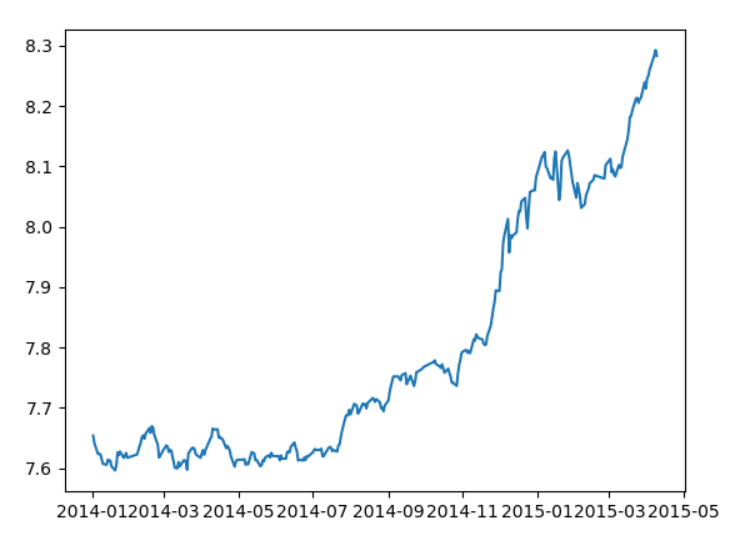
\includegraphics[height=5cm]{images/f000023}
\end{figure}
接着我们对该数据经过对数差分后,利用ARIMA来进行拟合,得到拟合模型为:
\begin{figure}[H]
	\caption{拟合后的ARIMA模型}
	\label{f000024}
	\centering
	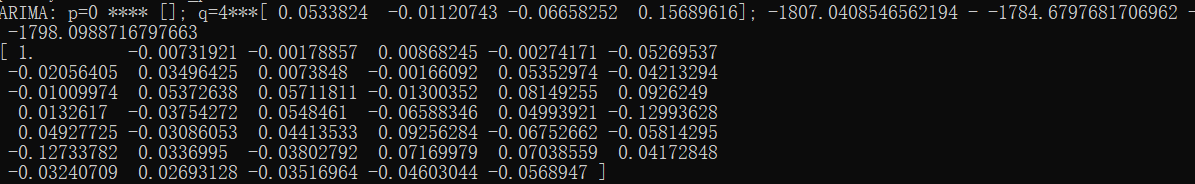
\includegraphics[height=2cm]{images/f000024}
\end{figure}
残差序列的自相关系数函数ACF图为:
\begin{figure}[H]
	\caption{残差序列的自相关系数函数ACF图}
	\label{f000025}
	\centering
	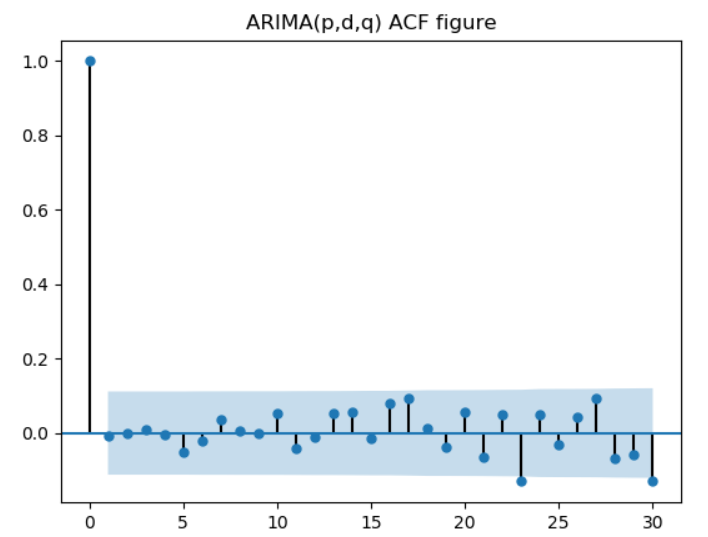
\includegraphics[height=5cm]{images/f000025}
\end{figure}
残差序列的偏自相关系数函数PACF图为:
\begin{figure}[H]
	\caption{残差序列的偏自相关系数函数PACF图}
	\label{f000026}
	\centering
	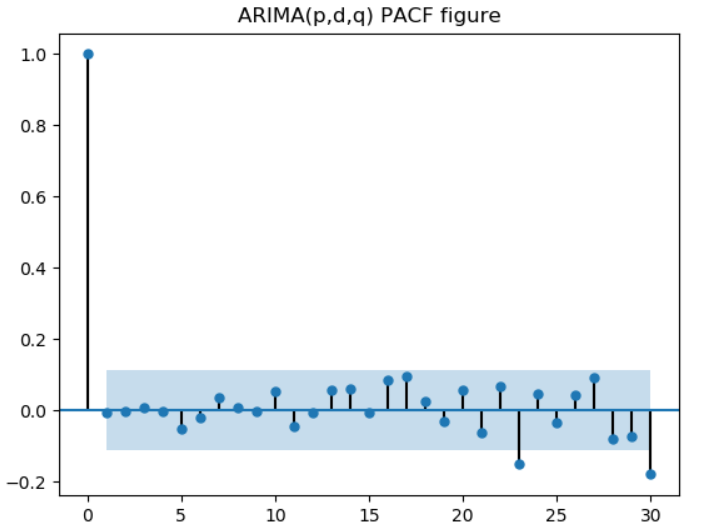
\includegraphics[height=5cm]{images/f000026}
\end{figure}
进行ADF检验的结果为:
\begin{figure}[H]
	\caption{ADF检验的结果}
	\label{f000027}
	\centering
	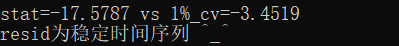
\includegraphics[height=1cm]{images/f000027}
\end{figure}
进行Ljung-Box检验结果为:
\begin{figure}[H]
	\caption{Ljung-Box检验结果}
	\label{f000028}
	\centering
	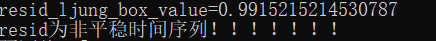
\includegraphics[height=1cm]{images/f000028}
\end{figure}
最后我们拿我们的模型进行预测,后三天的预测结果为:
\begin{figure}[H]
	\caption{ARIMA模型预测后三天结果}
	\label{f000029}
	\centering
	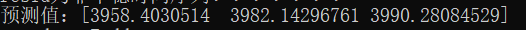
\includegraphics[height=0.6cm]{images/f000029}
\end{figure}
实际值为:
\begin{figure}[H]
	\caption{实际收盘价}
	\label{f000030}
	\centering
	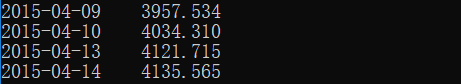
\includegraphics[height=2cm]{images/f000030}
\end{figure}
我们看到,我们的模型基本预测出了后三天的连涨行情,只不过上涨的幅度有一些小。

\maketitle\begin{center}
\Large \textbf{第3章 GARCH模型}
\end{center}
\begin{abstract}
在本章中我们将首先讲述条件异方差模型GARCH(Generalized AutoRegressive Conditional Heteroskedastic),
并将GARCH模型用于实际金融时间序列数据拟合。aqt002.py
\end{abstract}
\section{GARCH模型}
我们之前讨论的时序信号,都是假定其为平稳的。但是有很多时序信号,如某些商品的需求或价格,会随着季节的变化而发生变化,股票的价格为出现长时间的上涨或下跌趋势,在这些情况下,使用ARIMA模型的效果就不太好。对于我们要研究的股票数据,由于市场上很多交易是由大机构的算法来进行交易的,当出现价格明显示上涨或下跌时,会自动触发这些算法进行交易,从而放大了这种上涨或下跌趋势。这种情况我们称之为异方差,研究这种现象的方法我们称之为通用自回归条件异方差GARCH(Generalized AutoRegression Conditional Heteroskedasticity)模型。
\subsection{定义}
\subsubsection{ARCH模型}
我们先来看较为简单的自回归条件异方差ARCH模型,我们假设时序信号如下所示:
\begin{equation}
\epsilon _{t} = \sigma _{t} w_{t}
\label{e000050}
\end{equation}
其中$w_{t}$为白噪声序列,$\sigma _{t}$的定义如下所示:
\begin{equation}
\sigma _{t}^{2} = \alpha _{0} + \alpha _{1} \epsilon _{t-1}^{2}
\label{e000051}
\end{equation}
这个模型我们称之为ARCH(1)模型。我们以这个简单的模型为例,来说明ARCH(1)模型是对时序信号方差的变化进行建模。
我们首先来看时间序列$\{ \epsilon _{t} \}$的均值:
\begin{equation}
E(\epsilon _{t}) = E(\sigma _t w_{t}) = E(\sigma _{t})E(w_{t})=0
\label{e000052}
\end{equation}
我们再来看时间序列$\{ \epsilon _{t} \}$的方差:
\begin{equation}
\begin{aligned}
Var(\epsilon _{t}) = E\big( \epsilon _{t} - E(\epsilon _{t}) \big)^{2} =E\big( \epsilon _{t}^{2} - 2\epsilon _{t}E(\epsilon _{t}) + (E(\epsilon _{t}))^{2} \big) \\
=E(\epsilon _{t}^{2})-2E(\epsilon _{t})E(\epsilon _{t})+(E(\epsilon _{t}))^{2}=E(\epsilon _{t}^{2})-(E(\epsilon _{t}))^{2} \\
=E(\epsilon _{t}^{2})=E(\sigma _{t}^{2}w_{t}^{2})=E(\sigma _{t}^{2})E(w_{t}^{2})=E(\alpha _{0} + \alpha _{1}\epsilon _{t-1}^{2}) \\
=\aleph _{0} + \alpha _{1}E(\epsilon _{t-1}^{2})=\alpha _{0} + \alpha _{1}Var(\epsilon _{t-1})
\end{aligned}
\label{e000053}
\end{equation}
在上面的公式推导中,我们用到了$\{ w_{t} \}$为白噪声信号,其均值为0,方差为1。\newline
了解了基本ARCH模型之后,我们可以将ARCH(1)模型扩展到ARCH(p)模型,这里我们就不再展开了,将在下一节GARCH模型中进行详细介绍。
\subsubsection{GARCH模型}
对于时间序列信号$\{ \epsilon _{t} \}$其表达式为:
\begin{equation}
\epsilon _{t} = \sigma _{t} w_{t}
\label{e000054}
\end{equation}
其中$\{ w_{t} \}$为白噪声信号,其均值为0方差为1。其$\sigma _{t}^{2}$的定义为:
\begin{equation}
\sigma _{t}^{2} = \alpha _{0} + \sum_{i=1}^{p} \alpha _{i} \epsilon _{t-i}^{2} + \sum_{j=1}^{q} \beta _{j} \sigma _{t-j}^{2}
\label{e000055}
\end{equation}
其中$\alpha _{0}$、$\alpha _{i}$、$\beta _{j}$为参数。
\subsection{数据模拟}
为了对问题进行简化,我们在这里只模拟GARCH(1,1)模型,具体欲模拟的时间序列信号如下所示,在arch包的GARCH模型中,我们研究的信号为$r_{t}$,并且多出一个参数$\mu$:
\begin{equation}
\begin{aligned}
r_{t} = \epsilon _{t} + \mu \\
\epsilon _{t} = \sigma _{t}w_{t} \\
\sigma _{t}^{2} = \omega + \alpha _{1} \epsilon _{t-1}^{2} + \beta _{1} \sigma _{t-1}^{2}=0.2 + 0.5\epsilon _{t-1}^{2} + 0.3\sigma _{t-1}^{2}
\end{aligned}
\label{e000056}
\end{equation}
其程序如下所示:
\lstset{language=PYTHON, caption={GARCH拟合模拟数据}, label={c000008}}
\begin{lstlisting}
import sys
import math
import numpy as np
import pandas as pd
from pandas.plotting import register_matplotlib_converters
import matplotlib.pyplot as plt
import matplotlib.dates as mdates
from matplotlib.font_manager import FontProperties
from statsmodels.tsa import stattools
from statsmodels.graphics import tsaplots
from statsmodels.tsa.arima_model import ARIMA
import arch.unitroot as unitroot
import arch as arch

class Aqt002(object):
    def __init__(self):
        self.name = 'Aqt001'
        # 数据文件格式:编号 日期 星期几 开盘价 最高价 
        # 最低价 收益价 收益
        # Indexcd	Trddt	Daywk	Opnindex	Hiindex	
        # Loindex	Clsindex	Retindex
        self.data_file = 'data/pqb/aqt002_001.txt'
        
    def startup(self):
        print('GARCH模型...')
        np.random.seed(1)
        alpha0 = 0.2
        alpha1 = 0.5
        beta1 = 0.3
        samples = 10000 # 样本数量
        w = np.random.standard_normal(size=samples)
        epsilon = np.zeros((samples,), dtype=float)
        sigma = np.zeros((samples,), dtype=float)
        for i in range(2, samples):
            sigma_2 = alpha0 + alpha1 * math.pow(epsilon[i-1], 2) + \
                        beta1 * math.pow(sigma[i-1], 2)
            sigma[i] = math.sqrt(sigma_2)
            epsilon[i] = sigma[i]*w[i]
        plt.title('epsilon signal')
        plt.plot(epsilon)
        plt.show()
        # 绘制epsilonACFS
        acfs = stattools.acf(epsilon)
        tsaplots.plot_acf(epsilon, use_vlines=True, lags=30)
        plt.title('epsilon ACF')
        plt.show()
        # 绘制epsilon pow2 ACF
        acfs2 = stattools.acf(np.power(epsilon, 2))
        tsaplots.plot_acf(np.power(epsilon, 2), use_vlines=True, lags=30)
        plt.title('pow(epsilon,2) ACF')
        plt.show()
        # GARCH拟合
        am = arch.arch_model(epsilon, x=None, mean='Constant', 
                    lags=0, vol='Garch', p=1, o=0, q=1, 
                    power=2.0, dist='Normal', hold_back=None)
        model = am.fit(update_freq=0)
        # GARCH(1,1)参数
        print('############ GARCH(1,1)参数  ###################')
        print('model_type:{0}'.format(type(model)))
        print('mu={0:0.2f}; a0={1:0.2f}; a1={2:0.2f}; b1={3:0.2f}' \
                    .format(model.params['mu'], model.params['omega'], 
                    model.params['alpha[1]'], model.params['beta[1]']   ))
        print('###############################')
        #print(model.summary())
        # 残差信号
        plt.title('GARCH(1,1) resid')
        plt.plot(model.resid)
        plt.show()
        # 残差ACF
        resid_acf = stattools.acf(model.resid)
        tsaplots.plot_acf(model.resid, use_vlines=True, lags=30)
        plt.title('GARCH(1,1) resid ACF')
        plt.show()
        # ADF检验
        resid_adf = unitroot.ADF(model.resid)
        print('stat={0:0.4f} vs 1%_cv={1:0.4f}'.format( \
                    resid_adf.stat, resid_adf.critical_values['1%']))
        if resid_adf.stat < resid_adf.critical_values['1%']:
            print('resid为稳定时间序列 ^_^')
        else:
            print('resid为非稳定时间序列!!!!!')
        # Ljung-Box检验
        resid_ljung_box = stattools.q_stat(stattools.acf( \
                    model.resid)[1:12], len(model.resid))
        resid_lbv = resid_ljung_box[1][-1]
        print('resid_ljung_box_value={0}'.format(resid_lbv))
        # 0.05为显著性水平
        if resid_lbv < 0.05:
            print('resid为平稳时间序列 ^_^')
        else:
            print('resid为非平稳时间序列!!!!!!!')
        # 预测
        y = model.forecast(horizon=3)
        print('########### 预测值  ###############')
        print('len={0}; p1={1:0.3f}; p2={2:0.3f}; p3={3:0.3f}'. \
                    format(len(y.mean.iloc[-1]), y.mean.iloc[-1][0], 
                    y.mean.iloc[-1][1], y.mean.iloc[-1][2]))
        print('##########################')
\end{lstlisting}
我们欲拟合的时间序列信号为:
\begin{figure}[H]
	\caption{拟拟合的时间序列}
	\label{f000031}
	\centering
	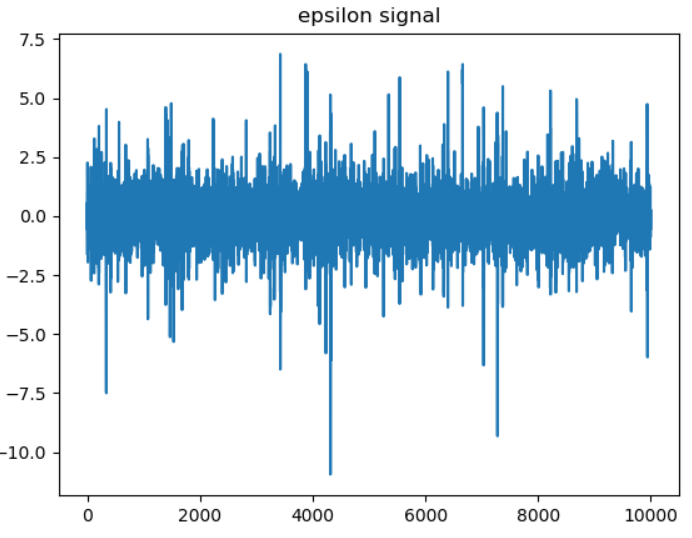
\includegraphics[height=2cm]{images/f000031}
\end{figure}
该时间序列的自相关系数函数ACF图:
\begin{figure}[H]
	\caption{epsilon的自相关系数函数ACF图}
	\label{f000032}
	\centering
	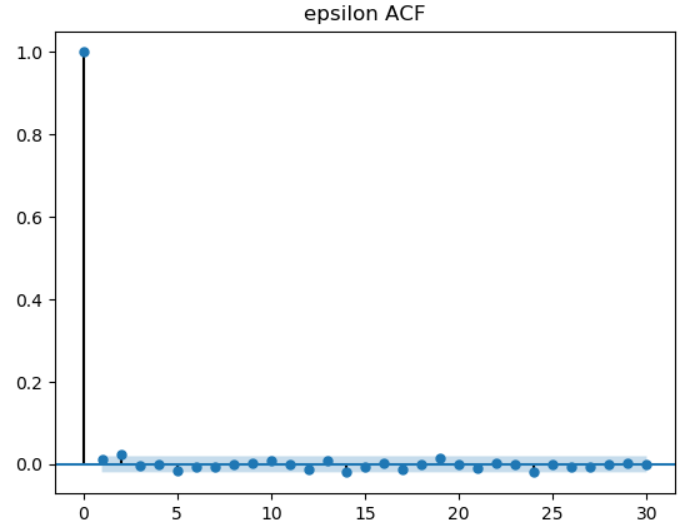
\includegraphics[height=2cm]{images/f000032}
\end{figure}
由上图可以看出,其基本是一个平稳时间序列。我们取其平方,其自相关系数函数ACF图如下所示:
\begin{figure}[H]
	\caption{pow(epsilon,2)的自相关系数函数ACF图}
	\label{f000033}
	\centering
	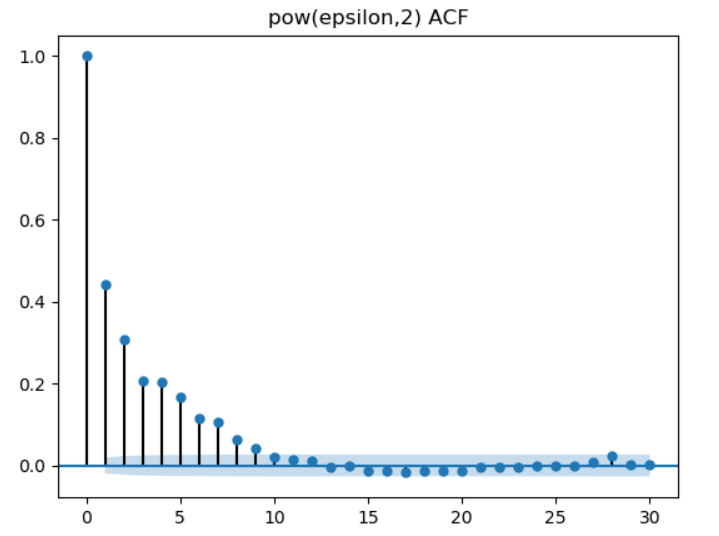
\includegraphics[height=2cm]{images/f000033}
\end{figure}
由上图可以看出,将其平方后,其就是不平稳的时间序列了。GARCH模型就是来处理这种情况的。\newline
我们采用GARCH进行拟合后,得到的残差信号为:
\begin{figure}[H]
	\caption{GARCH(1,1)残差序列}
	\label{f000034}
	\centering
	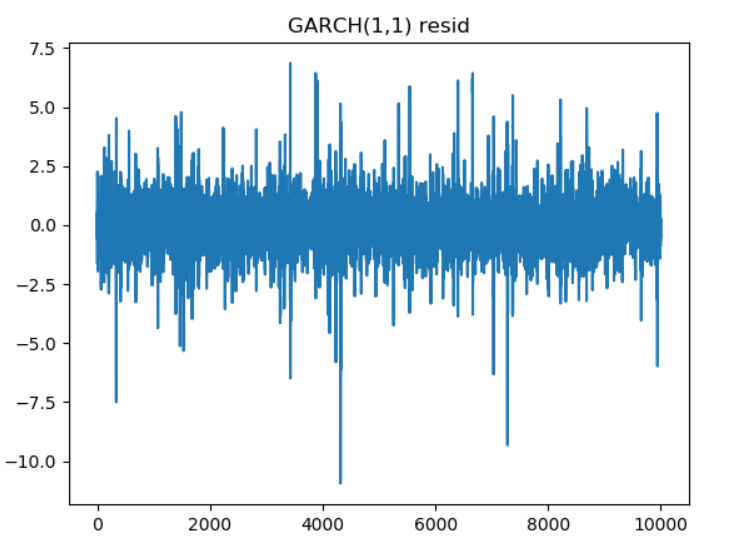
\includegraphics[height=2cm]{images/f000034}
\end{figure}
残差信号的自相关系数函数ACF图为:
\begin{figure}[H]
	\caption{GARCH(1,1)残差序列自相关系数函数ACF图}
	\label{f000035}
	\centering
	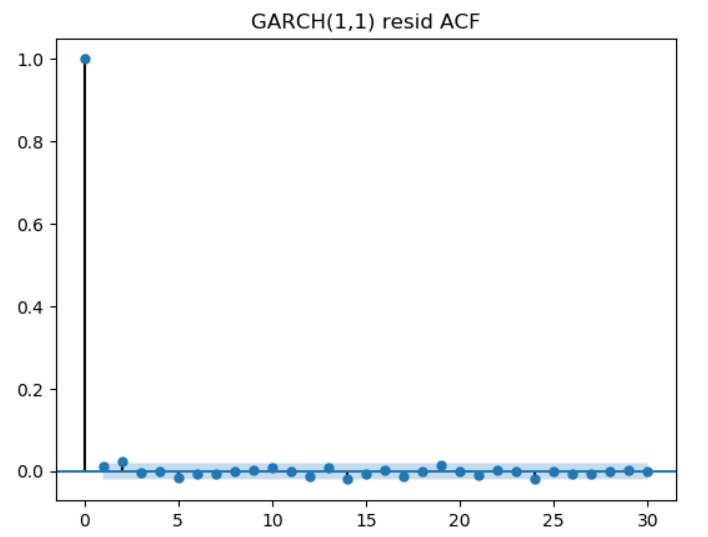
\includegraphics[height=2cm]{images/f000035}
\end{figure}
程序的运行结果如下所示:
\begin{figure}[H]
	\caption{程序运行结果}
	\label{f000036}
	\centering
	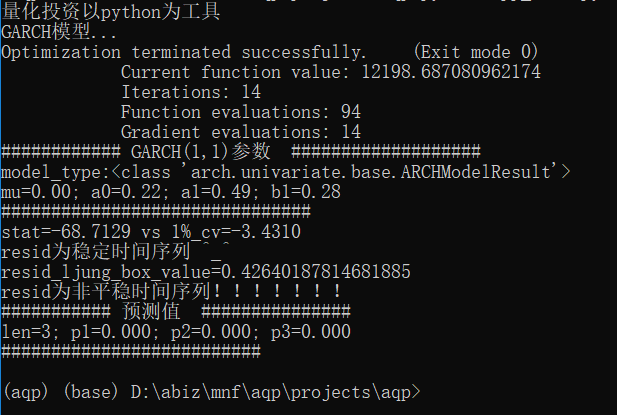
\includegraphics[height=2cm]{images/f000036}
\end{figure}
由上图可知,我们对GARCH(1,1)模型的参数预测还是相当准确的,说明我们方法是正确的。
\subsection{金融数据拟合}
下面我们以上证综指的收盘价为例,来讨论GARCH拟合预测后三天股价问题。对于收盘价这样的信号,我们仍然采用对数一阶差分形式来作为建模的时间序列,我们用GARCH(3,2)来进行拟合,程序如下所示:
\lstset{language=PYTHON, caption={GARCH拟合并预测上证综指收盘价}, label={c000009}}
\begin{lstlisting}
    def garch_finance_demo(self):
        print('拟合上证综指收盘价...')
        register_matplotlib_converters()
        data = pd.read_csv(self.data_file, sep='\t', index_col='Trddt')
        sh_index = data[data.Indexcd==1]
        sh_index.index = pd.to_datetime(sh_index.index)
        sh_return = sh_index.Retindex
        # raw_data = sh_index.Retindex
        raw_data = sh_index.Clsindex
        train_data = raw_data[:-3]
        dcp = np.log(train_data).diff(1)[1:] 
        plt.plot(dcp)
        plt.show()
        # GARCH拟合
        am = arch.arch_model(dcp, x=None, mean='Constant', 
                    lags=0, vol='Garch', p=3, o=0, q=2, 
                    power=2.0, dist='Normal', hold_back=None)
        model = am.fit(update_freq=0)
        # GARCH(1,1)参数
        print('############ GARCH(1,1)参数  ###################')
        '''
        print('mu={0:0.2f}; a0={1:0.2f}; a1={2:0.2f}; a2={3:0.2f}, b1={4:0.2f}, b2={5:0.2f}' \
                    .format(model.params['mu'], model.params['omega'], 
                    model.params['alpha[1]'], model.params['alpha[2]'], model.params['beta[1]'], model.params['beta[2]']   ))
        '''
        print('###############################')
        resid = model.resid
        # 绘制ACF
        acfs = stattools.acf(resid)
        print(acfs)
        tsaplots.plot_acf(resid, use_vlines=True, lags=30)
        plt.title('GARCH(p,q) ACF figure')
        plt.show()
        '''
        pacfs = stattools.pacf(resid)
        print(pacfs)
        tsaplots.plot_pacf(resid, use_vlines=True, lags=30)
        plt.title('ARIMA(p,d,q) PACF figure')
        plt.show()
        '''
        # ADF检验
        resid_adf = unitroot.ADF(resid)
        print('stat={0:0.4f} vs 1%_cv={1:0.4f}'.format(resid_adf.stat, resid_adf.critical_values['1%']))
        if resid_adf.stat < resid_adf.critical_values['1%']:
            print('resid为稳定时间序列 ^_^')
        else:
            print('resid为非稳定时间序列!!!!!')
        # Ljung-Box检验
        resid_ljung_box = stattools.q_stat(stattools.acf(resid)[1:12], len(resid))
        resid_lbv = resid_ljung_box[1][-1]
        print('resid_ljung_box_value={0}'.format(resid_lbv))
        # 0.05为显著性水平
        if resid_lbv < 0.05:
            print('resid为平稳时间序列 ^_^')
        else:
            print('resid为非平稳时间序列!!!!!!!')
        # 预测
        frst = model.forecast(horizon=3)
        y = frst.mean.iloc[-1]
        print('预测值:{0}'.format(y))
        p1 = math.exp(math.log(train_data[-1]) + y[0])
        p2 = math.exp(math.log(p1) + y[1])
        p3 = math.exp(math.log(p2) + y[2])
        print('        预测值    实际值  (3957.534)')
        print('第一天:{0} vs 4034.310'.format(p1))
        print('第二天:{0} vs 4121.715'.format(p2))
        print('第三天:{0} vs 4135.565'.format(p3))
\end{lstlisting}
我们要建模的上证综指收盘价对数差分信号如下所示:
\begin{figure}[H]
	\caption{上证综指收盘价对数差分信号}
	\label{f000037}
	\centering
	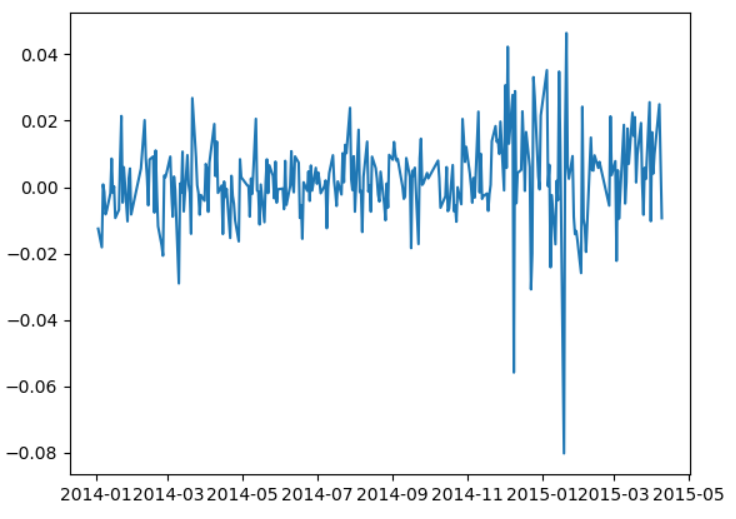
\includegraphics[height=2cm]{images/f000037}
\end{figure}
经过GARCH(3,2)拟合后的残差信号:
\begin{figure}[H]
	\caption{上证综指收盘价对数差分信号}
	\label{f000038}
	\centering
	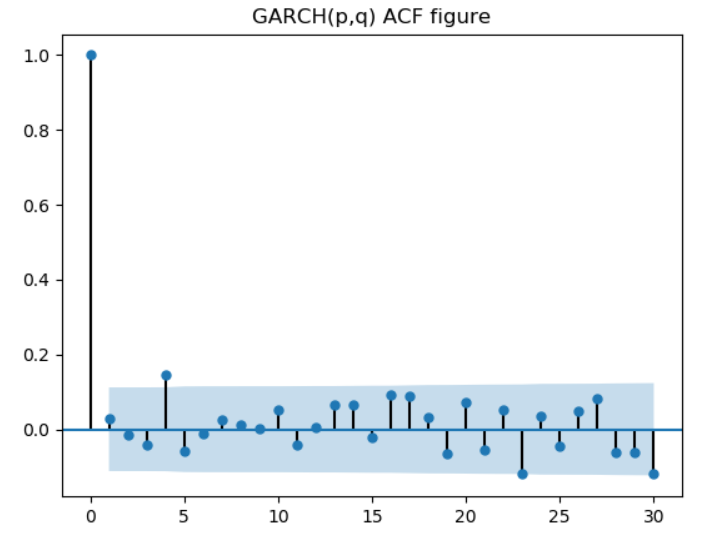
\includegraphics[height=2cm]{images/f000038}
\end{figure}
由图可见,其基本是一个平稳时间序列,可以用来进行预测。但是我们ADF检验表明其是平稳时间序列,但是Ljung-Box检验表明其不是时间平稳时间序列,因此我们还需要仔细分析其中的原因。程序运行结果如下所示:
\begin{figure}[H]
	\caption{程序运行结果}
	\label{f000039}
	\centering
	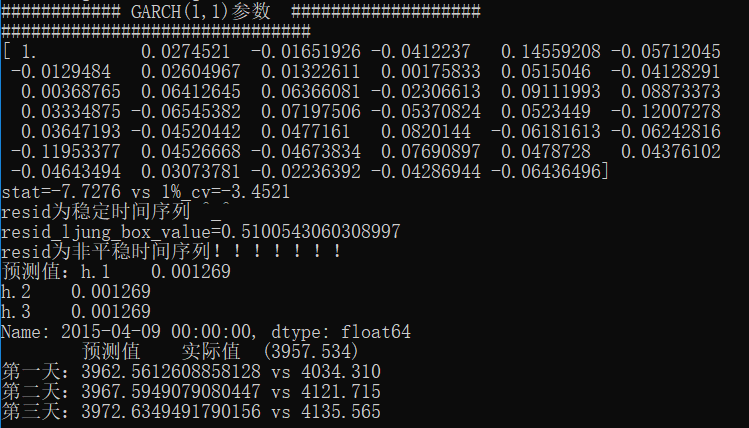
\includegraphics[height=2cm]{images/f000039}
\end{figure}
由上图可以看出,预测结果也基本捕捉到了后三天连涨趋势,只是涨幅估计偏低,这证明我们采用GARCH(p,q)模型来预测是可行的。





























\maketitle\begin{center}
\Large \textbf{第4章 协整模型}
\end{center}
\begin{abstract}
在本章中我们将首先讲述交易对的概念,并讲述如何利用交易对的均值回归特性,通过对交易对的多空操作,实现稳定的盈利。在本章中,我们主要讲解交易对的数学原理,怎样确定对冲比例。对于怎样利用交易对进行统计套利策略研发,将在后续章节中介绍。aqt003.py
\end{abstract}
\section{协整模型}
本章讲述的内容是统计套利策略,这是一种市场中性策略,无论是市场是涨是跌,均有可能盈利。将统计套利用到极致的例子,应该属于上世纪90年代的LTCM基金。LTCM基金成立于1994年,成立时基金规模为12.5亿美金,但是到1997年,基金规模就达到了48亿美金,是当时世界上四大基金之一。LTCM基金的创始人是金牌交易员,合伙人是顶级统计学家,他们发现德国国债和意大利国债有一个稳定的比例关系,大概率波动的机率会非常小,因此当德国国债上涨时,德国国债与意大利国债之比将增大,大幅度偏离均值,他们就卖出德国国债,买入意大利国债,一段时间之后,德国国债会下跌,德国国债和意大利国债之比就会回归到均值,此时他们卖出之前买入的意大利国债,重新买入之前卖出的德国国债,这样他们持有德国国债和意大利国债没有发生变化,但是却赚到了这次波动差价所产生的利润。利用这种方式,LTCM基金获得了巨大的成功。然而LTCM基金的神话终结于1997年,主要有以下几个原因:首先LTCM认为德国国债和意大利国债之比符合正态分布,但是虽然自然界大部分复杂的现象都是正态分布,但是人类社会现象,却不一定是正态分布,黑天鹅事件也许是长态,在1997年,东南亚发生了金融危机,俄罗斯发生了国债违约,正是这两个黑天鹅事件,使德国国债与意大利国债之比不再符合正态分布,而LTCM基金由于对这些事件缺乏预见性,而遭受了巨大的损失;同时,在LTCM基金破产之后,人们看LTCM基金的财务数据发现,其资金杠杆高达数万倍,因此一次失误的决策,就足以使整个公司破产。由这个实例我们可以看出,基于交易对均值回归的统计回归策略,具有巨大的盈利潜力,同时我们也应看到,杠杆是魔鬼,任何策略中最重要的都是资金和仓位管理。\newline
交易对不仅在传统金融市场,如股市、期货、外汇、债市上存在,在新兴的加密货币市场,也是一种非常重要的策略,前一两年兴起的比特币搬砖模式,就是交易对策略在加密货市场的应用。
\subsection{数据模拟}
\subsubsection{协整模型构建}
根据\cite{r000002}的内容,我们可以通过模拟数据来加深我们对基本概念的理解。假设$\{ w_{t} \}$为白噪声,在此基础上定义随机游走信号:
\begin{equation}
z_{t} = z_{t-1} + w_{t}
\label{e000058}
\end{equation}
在此基础上我们定义两个非平稳的时间序列信号:
\begin{equation}
x_{t} = pz_{t} + w_{t} = 0.3z_{t} + w_{t}
\label{e000059}
\end{equation}
\begin{equation}
y_{t} = qz_{t} + w_{t} = 0.6z_{t} + w_{t}
\label{e000060}
\end{equation}
如果我们将$\{ x_{t} \}$和$\{ y_{t} \}$进行线性组合:
\begin{equation}
ax_{t} + by_{t} = (ap+bq)z_{t} + w_{t} = (0.3a+0.6b)z_{t} + w_{t}
\label{e000061}
\end{equation}
如果$0.3a+0.6b=0$的话,那么$\{ x_{t} \}$和$\{ y_{t} \}$的这个线性组合就只剩下白噪声信号,因此其是
平稳时间序列信号,因此当$a=2, b=-1$时,这个序列就是平稳时间序列信号。\newline
根据这一思想,程序如下所示:
\lstset{language=PYTHON, caption={线性组合形成平稳时间序列}, label={c000010}}
\begin{lstlisting}
    def simulate_demo(self):
        '''
        模拟数据生成
        '''
        # 生成白噪声信号
        samples = 1000
        w = np.random.standard_normal(size=samples)
        # 生成随机游走序列
        z = np.zeros((samples,))
        for t in range(1, samples):
            z[t] = z[t-1] + w[t]
        # 生成非平稳信号,即交易对x和y
        x = np.zeros((samples,))
        y = np.zeros((samples,))
        p = 0.3
        q = 0.6
        for t in range(samples):
            x[t] = p*z[t] + w[t]
            y[t] = q*z[t] + w[t]
        fig = plt.figure(figsize=(6, 6))
        w_plt = plt.subplot(2, 2, 1, title='White Noise: w')
        w_plt.plot(w)
        z_plt = plt.subplot(2, 2, 2, title='Random Walk: z')
        z_plt.plot(z)
        x_plt = plt.subplot(2, 2, 3, title='Non Stationary Signal: x')
        x_plt.plot(x)
        y_plt = plt.subplot(2, 2, 4, title='Non Stationary Signal: y')
        y_plt.plot(y)
        fig.tight_layout()
        plt.show()
        # 生成协整信号
        a = 2
        b = -1
        c = a * x + b * y
        plt.plot(c)
        plt.title('Cointegration Model')
        plt.show()
        # 采用ADF检验 
        resid_adf = unitroot.ADF(c)
        print('stat={0:0.4f} vs 1%_cv={1:0.4f}'.format( \
                    resid_adf.stat, resid_adf.critical_values['1%']))
        if resid_adf.stat < resid_adf.critical_values['1%']:
            print('resid为稳定时间序列 ^_^')
        else:
            print('resid为非稳定时间序列!!!!!')
\end{lstlisting}
我们首先绘制出白噪声、随机游走和x及y信号:
\begin{figure}[H]
	\caption{研究序列}
	\label{f000042}
	\centering
	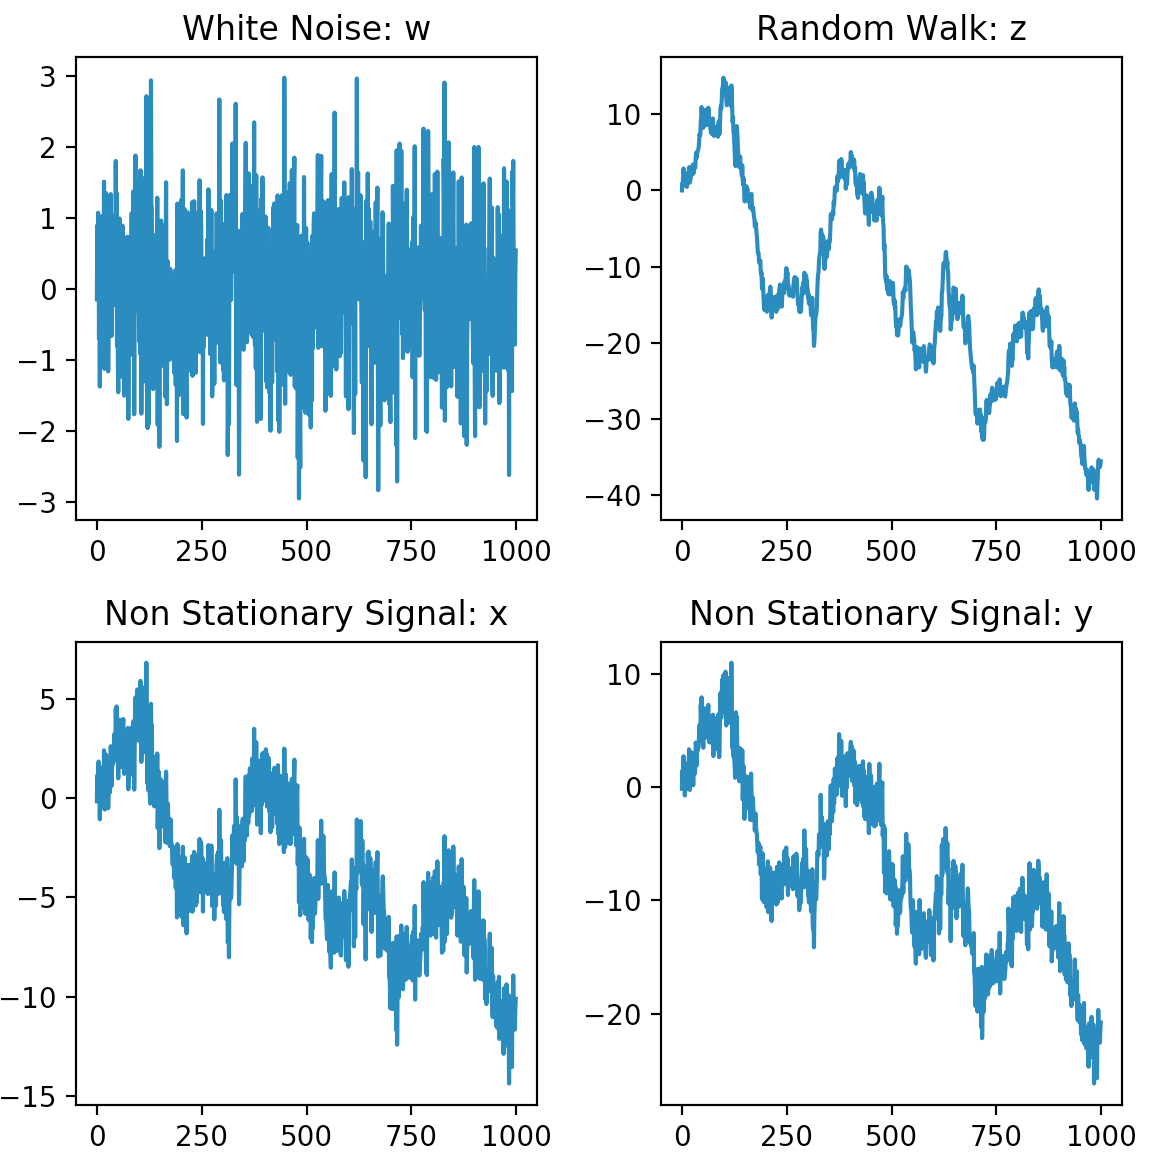
\includegraphics[height=5cm]{images/f000042}
\end{figure}
接着我们绘制出x和y的线性组合:
\begin{figure}[H]
	\caption{x和y的线性组合}
	\label{f000043}
	\centering
	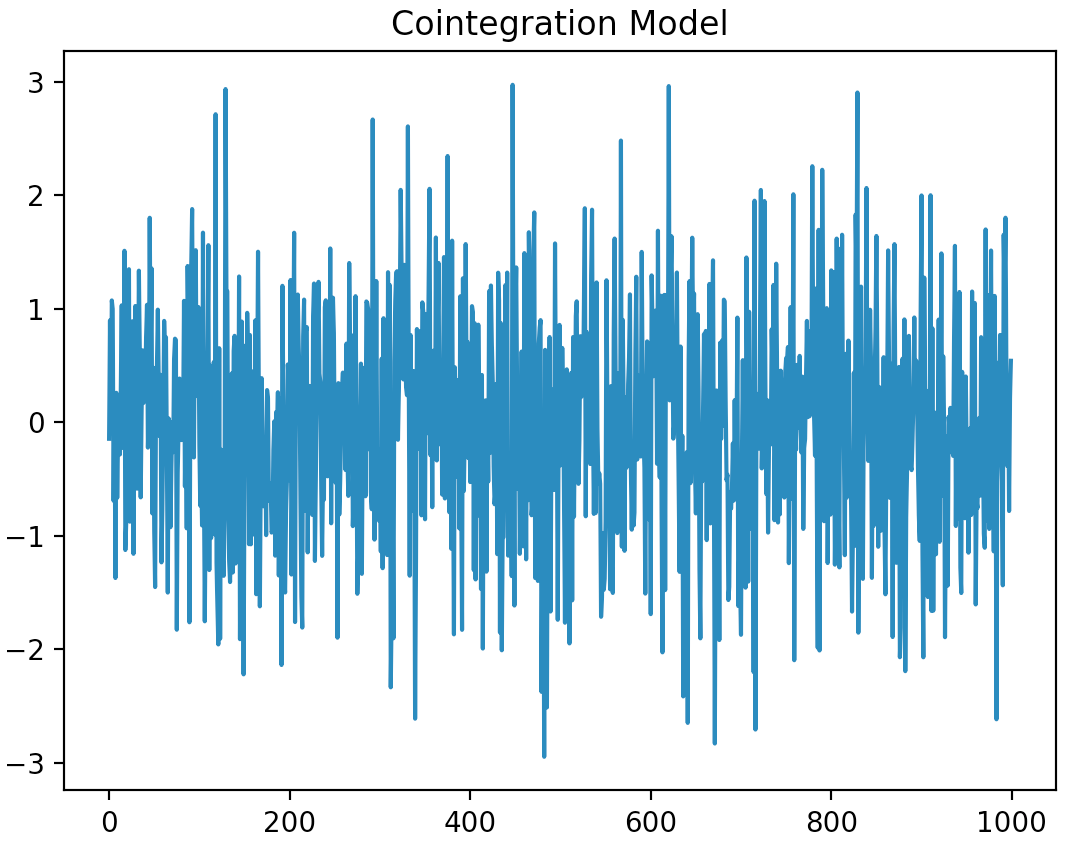
\includegraphics[height=5cm]{images/f000043}
\end{figure}
我们利用ADF检验其稳写性:
\begin{figure}[H]
	\caption{ADF检验}
	\label{f000044}
	\centering
	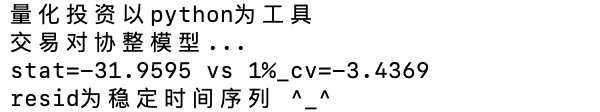
\includegraphics[height=1cm]{images/f000044}
\end{figure}
由上面的ADF检验可以看出,x和y的线性组合与理论分析一致,是平稳时间序列。
\subsubsection{对冲比例确定}
在上面的例子中,我们验证了我们的假设,即对两个非平稳的时间序列进行线性组合,通过选择合适的系数,可以得到平稳时间序
列信号。现在的问题就变为怎样求出这些系数,使线性组合后的时间序列具有平稳性。在这一节中,我们将向大家演示采用线性
回归技术,来求出线性组合的系数。虽然线性回归算法非常简单,尤其是我们这里只有一维,就更简单了。但是这里我们将采用
Google在今年3月新推出的TensorFlow 2.0 alpha,采用高级API keras来完成这一过程。\newline
\paragraph{线性回归模型}
在讲解确定线性组合系数之前,我们先来讲解一下为达到这一目的所开发的基于TensorFlow 2.0的线性回归模型。代码如下所示:
\lstset{language=PYTHON, caption={基于TensorFlow 2.0的线性回归模型}, label={c000011}}
\begin{lstlisting}
    import numpy as np
    import matplotlib.pyplot as plt
    import tensorflow as tf
    
    class QciLinearRegression(object):
        def __init__(self, train_x=None, train_y=None, 
                    validate_x=None, validate_y=None, 
                    test_x=None, test_y=None):
            self.name = 'QciLinearRegression'
            self.loss = 'mean_squared_error'
            self.learning_rate = 0.01
            self.optimizer = tf.keras.optimizers.Adam(self.learning_rate)
            self.epoch = 50000
            if train_x:
                self.train_x = train_x
                self.train_y = train_y
                self.validate_x = validate_x
                self.validate_y = validate_y
                self.test_x = test_x
                self.test_y = test_y
            else:
                self.train_x, self.train_y, self.validate_x, \
                            self.validate_y, self.test_x, \
                            self.test_y = self.generate_dataset()
    
        def generate_dataset(self):
            train_x = np.array([-40, -10, 0, 8, 15, 22, 38, 20, 9, 13], dtype=float)
            train_y = np.array([-40, 14, 32, 46, 59, 72, 100, 68, 48.2, 55.4], dtype=float)
            validate_x = np.array([], dtype=float)
            validate_y = np.array([], dtype=float)
            test_x = np.array([], dtype=float)
            test_y = np.array([], dtype=float)
            return train_x, train_y, validate_x, validate_y, test_x, test_y
    
        def train(self):
            model = self.build_model()
            model.compile(loss=self.loss, optimizer=self.optimizer)
            class PrintDot(tf.keras.callbacks.Callback):
                def on_epoch_end(self, epoch, logs):
                    if epoch % 100 == 0: print('')
                    print('epoch:{0}...{1}!'.format(epoch, logs))
            early_stop = tf.keras.callbacks.EarlyStopping(monitor='val_loss', patience=10)
            history = model.fit(self.train_x, self.train_y, 
                        epochs=self.epoch, validation_split = 0.1,  
                        verbose=False, callbacks=[early_stop, PrintDot()])
            plt.title('linear regression training process')
            plt.xlabel('epochs')
            plt.ylabel('error')
            plt.plot(history.history['loss'])
            plt.show()
            model.save('./work/aqt003_qiclr')
            weights = np.array(model.get_weights())
            print(weights)
    
        def build_model(self):
            layer1 = tf.keras.layers.Dense(units=1, input_shape=[1])
            model = tf.keras.Sequential([layer1])
            return model
    
        def predict(self, data):
            model = tf.keras.models.load_model('./work/aqt003_qiclr')
            rst = model.predict(data)
            return rst
    
    if '__main__' == __name__:
        lr = QciLinearRegression()
        lr.train()    
\end{lstlisting}
初始化函数的参数为训练样本集、验证样本集和测试样本集,缺省值为空,当不传递这些值时,我们采用类内定义的
generate\_dataset方法来为这些属性赋值。同时,在构造函数中设定了代价函数为最小平方误差函数,学习率为0.01,优化
算法为最常用的Adam,训练遍数为5万。\newline
在generate\_dataset函数中,我们输入特征为摄氏度的温度,而输出值为华氏度的温度,二者的关系为:
\begin{equation}
F = 1.8 \times C + 32
\label{e000062}
\end{equation}
我们任务就是学出1.8和32这两个参数。\newline
外部程序通过调用train方法作为入口,程序首先调用build\_model方法生成模型,我们的这个网络由两层组成,第1层为输入层
只有一个节点,第2层为输出层,其也只有一个节点,这个网络的参数为:第1层节点到第2层节点的连接权值和第2层神经元的偏置
值。创建完模型之后,我们通过model.compile来设置模型的代价函数和优化算法;为了提高模型的泛化能力避免overfitting,
我们采用early stopping算法,当验证集上的精度在10个循环中没有明显改进时,停止训练过程(在后面的日志中,我们可以看到
虽然我们定义训练5万次,但是实际训练不到1万次就停止了)。接着我们定义一个临时类,因为神经网络训练
通常会很耗时,我们用这个函数打印当前进度情况。接着我们调用model.fit来开始实际训练过程,在后台日志中我们可以看到,误差
会逐渐减少,如图所示:
\begin{figure}[H]
	\caption{程序运行日志}
	\label{f000045}
	\centering
	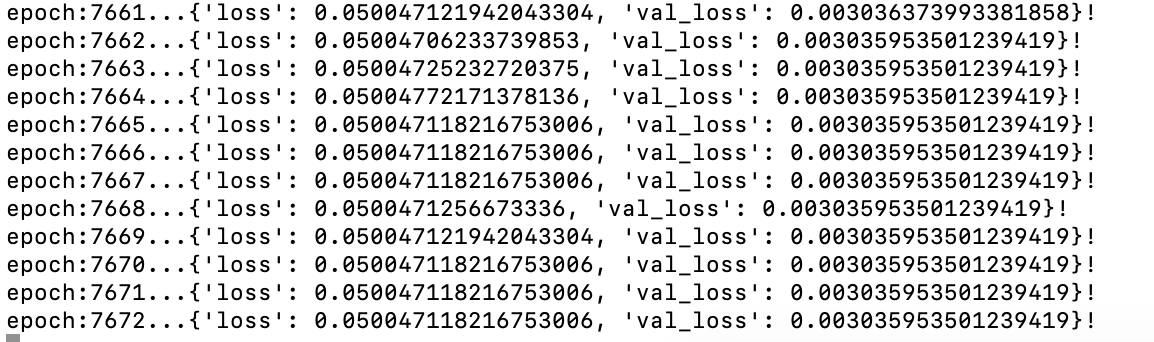
\includegraphics[height=3cm]{images/f000045}
\end{figure}
我们可以看到最后一列的验证集上的误差在10次没有明显变化时,由于early stopping算法,训练过程就自动结束了。接下来我们
可以绘制出误差随训练时间的变化过程,如下所示:
\begin{figure}[H]
	\caption{误差变化曲线}
	\label{f000046}
	\centering
	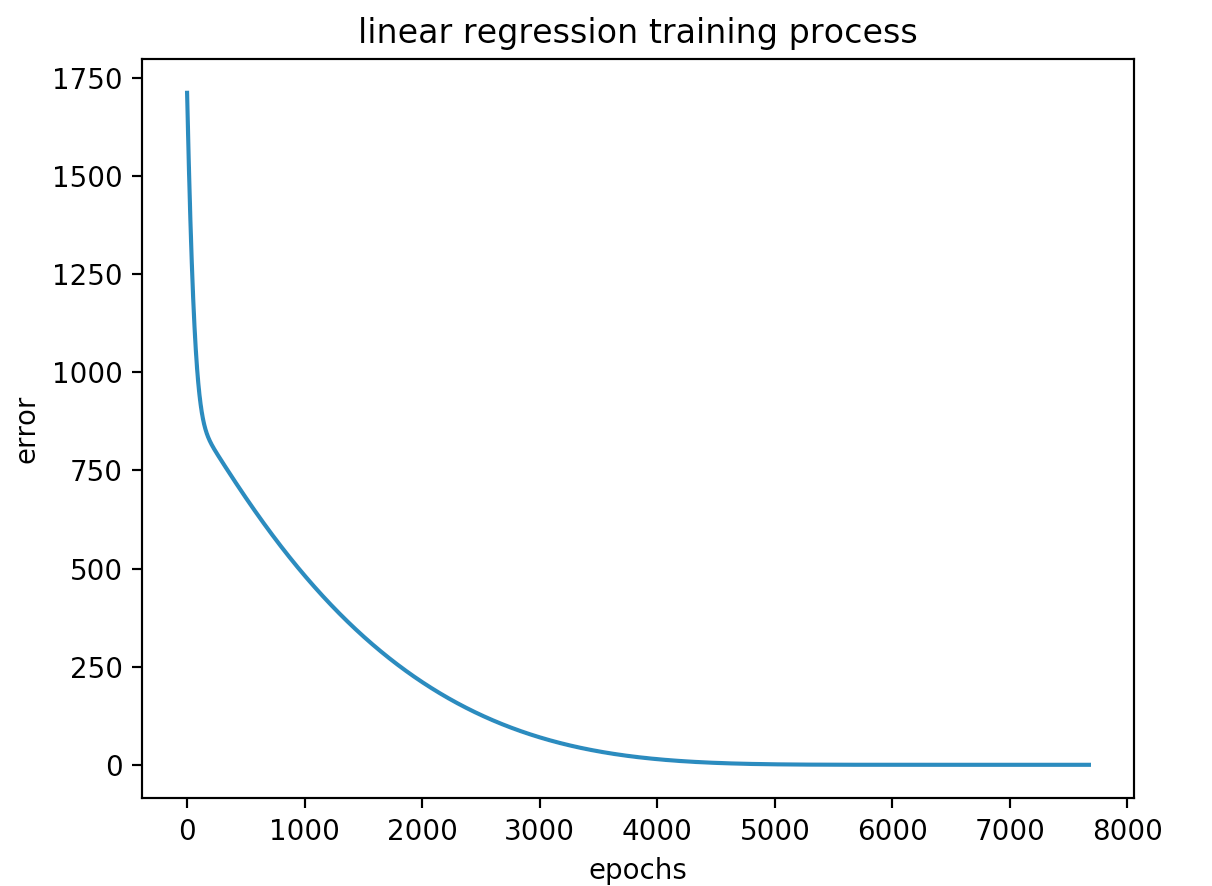
\includegraphics[height=1cm]{images/f000046}
\end{figure}
最终学到的参数值为:
\begin{figure}[H]
	\caption{误差变化曲线}
	\label{f000047}
	\centering
	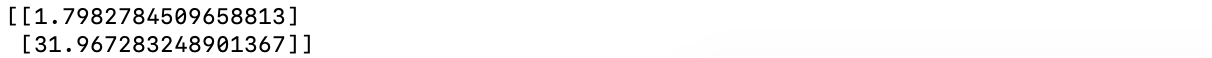
\includegraphics[height=1cm]{images/f000047}
\end{figure}
我们看到其与实际值就非常接近了,证明我们线性回归模型是正确的。虽然在我们协整模型中用不到,但是我们还是介绍一下当网络训
练完成之后,下一步就给出数据,让其给我们算出真实的结果,这在predict方法中实现。在predict方法中,首先从模型文件中
恢复出网络结构,然后运行模型的predict方法生成并返回预测值,调用代码如下所示:
\lstset{language=PYTHON, caption={利用线性回归模型进行预测}, label={c000012}}
\begin{lstlisting}
    data = np.array([[100.0]], dtype=float)
    rst = qcilr.predict(data)
    print(rst)
\end{lstlisting}
运行结果如下所示:
\begin{figure}[H]
	\caption{预测值}
	\label{f000048}
	\centering
	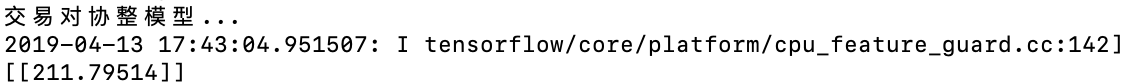
\includegraphics[height=1cm]{images/f000048}
\end{figure}
\paragraph{对冲比例确定}
在有了线性回归模型之后,下面我们就用线性回归模型来确定对冲比例。程序如下所示:
\lstset{language=PYTHON, caption={线性回归模型确定对冲比例}, label={c000013}}
\begin{lstlisting}
    def qcilr_demo(self):
        # 生成白噪声信号
        samples = 1000
        w = np.random.standard_normal(size=samples)
        # 生成随机游走序列
        z = np.zeros((samples,))
        for t in range(1, samples):
            z[t] = z[t-1] + w[t]
        # 生成非平稳信号,即交易对x和y
        x = np.zeros((samples,))
        y = np.zeros((samples,))
        p = 0.3
        q = 0.6
        for t in range(samples):
            x[t] = p*z[t] + w[t]
            y[t] = q*z[t] + w[t]
        fig = plt.figure(figsize=(6, 6))
        w_plt = plt.subplot(2, 2, 1, title='White Noise: w')
        w_plt.plot(w)
        z_plt = plt.subplot(2, 2, 2, title='Random Walk: z')
        z_plt.plot(z)
        x_plt = plt.subplot(2, 2, 3, title='Non Stationary Signal: x')
        x_plt.plot(x)
        y_plt = plt.subplot(2, 2, 4, title='Non Stationary Signal: y')
        y_plt.plot(y)
        fig.tight_layout()
        plt.show()
        # 以x作为自变量
        w1, x_y_p = self.do_linear_regression(x, y)
        # 将y作为自变量
        w2, y_x_p = self.do_linear_regression(y, x)
        print('xToy={0}({1}) vs yTox={2}({3})'.format(x_y_p, w1[0][0], y_x_p, w2[0][0]))
        if x_y_p < y_x_p:
            print('######## x  为自变量')
            c = w1[0][0] * x - y
        else:
            print('######### y  为自变量')
            c = w2[0][0] * y - x
        plt.title('Final Cointegration Signal')
        plt.plot(c)
        plt.show()
\end{lstlisting}
在上面的程序中,我们首先像上一节一样,先做出x和y两个非平稳的时间序列信号,然后我们先以x为自变量做一次线性回归,
求出ADF检验的p值和对冲比例,再以y作为自变量做一次线性回归,求出ADF检验的值p和对冲比例,我们取ADF检验的p值较小的
一个作为最终结果,求出线性组合的信号c,最后绘制出其信号典线。\newline
原始信号如下所示:
\begin{figure}[H]
	\caption{原始信号}
	\label{f000049}
	\centering
	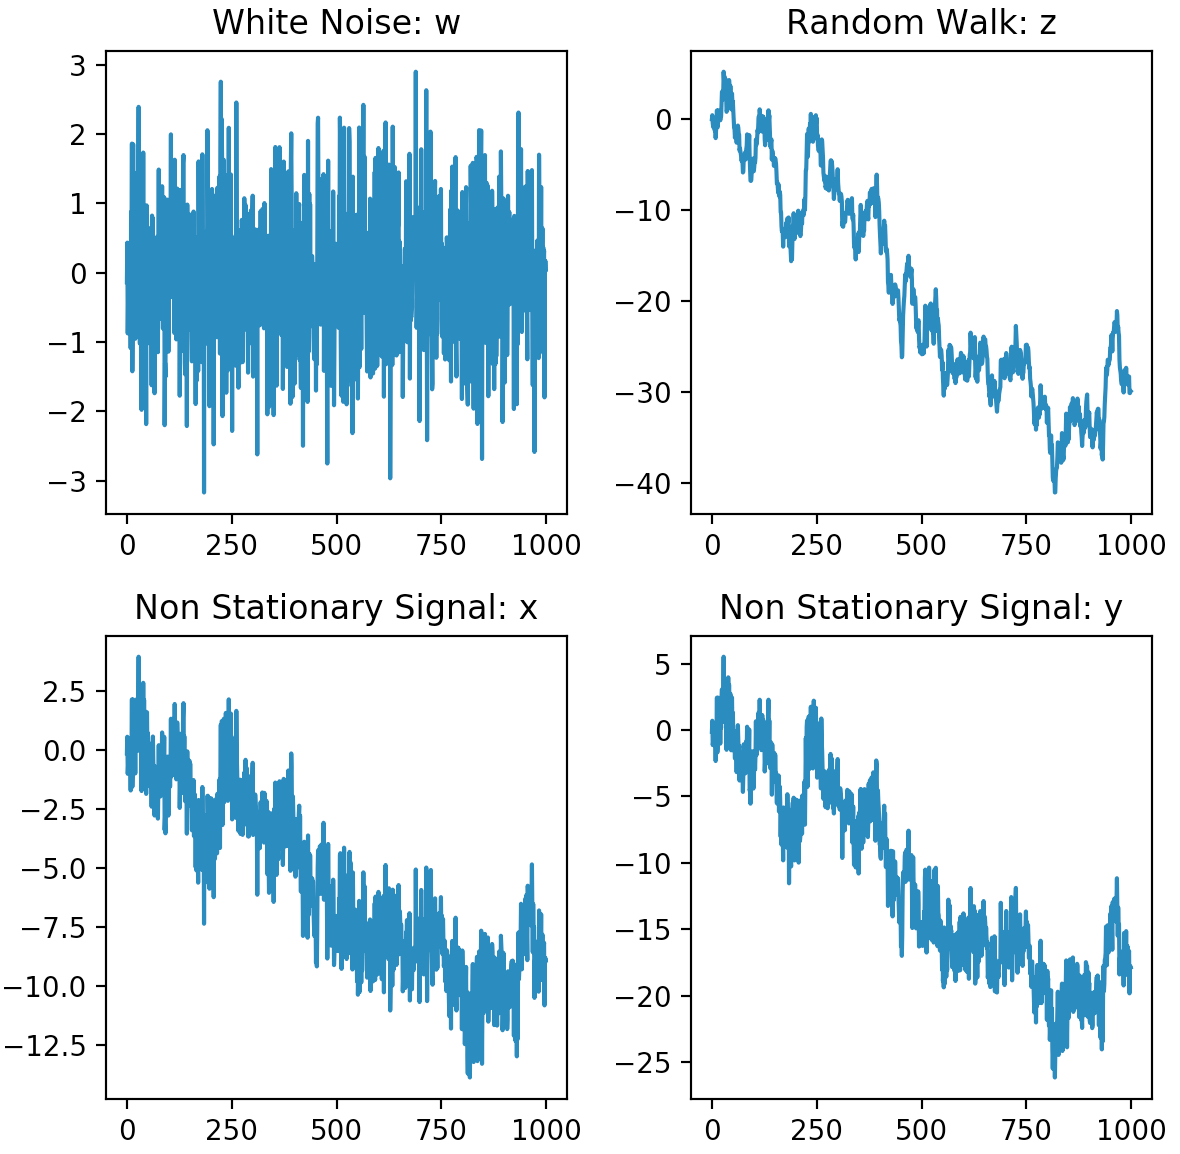
\includegraphics[height=5cm]{images/f000049}
\end{figure}
以x为自变量时线性回归运行情况:
\begin{figure}[H]
	\caption{以x为自变量的线性回归}
	\label{f000050}
	\centering
	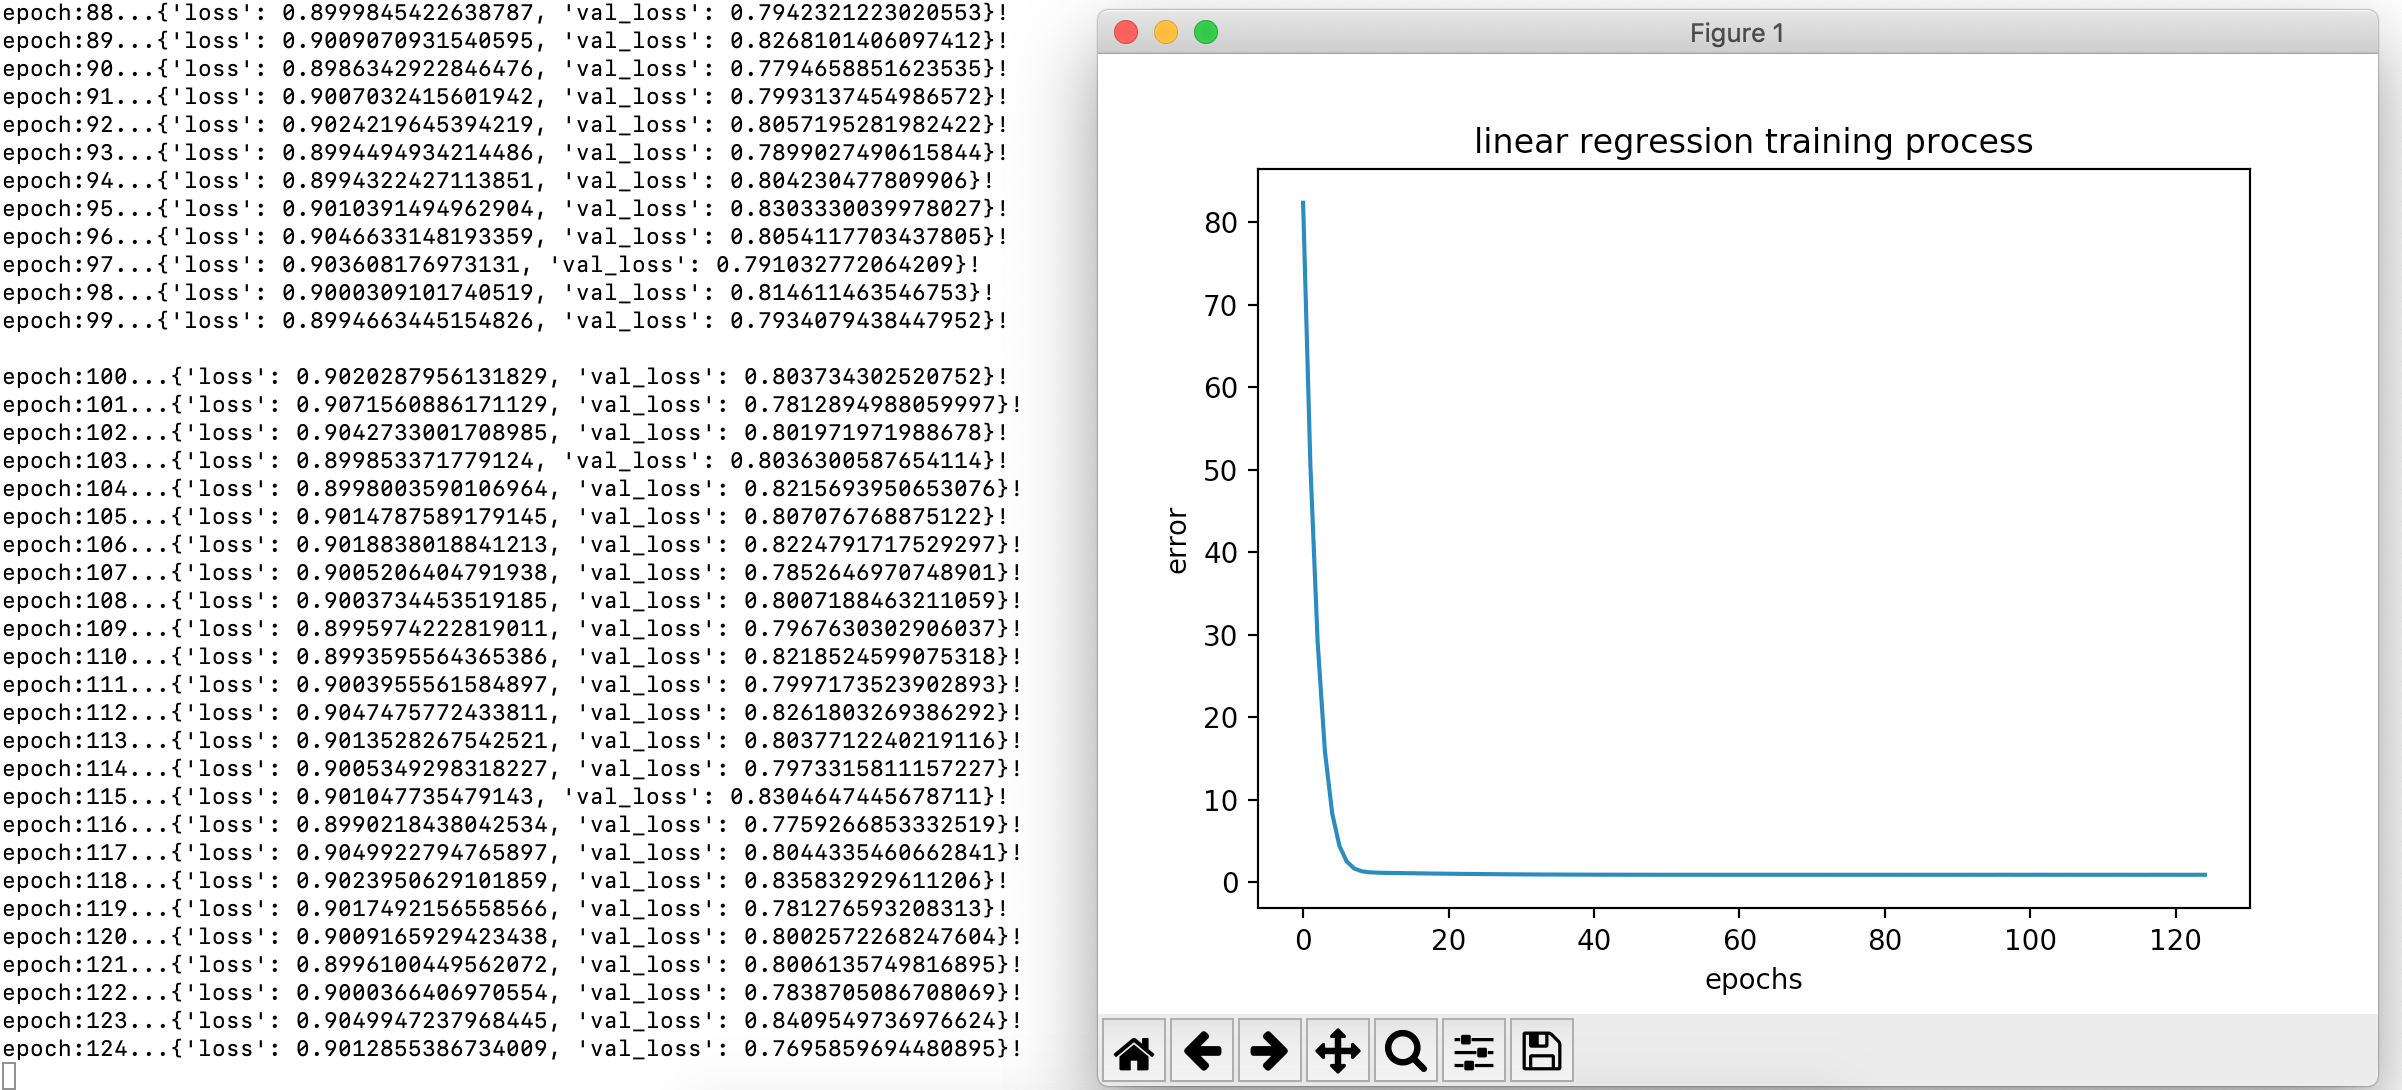
\includegraphics[height=5cm]{images/f000050}
\end{figure}
以y为自变量时线性回归运行情况:
\begin{figure}[H]
	\caption{以y为自变量时线性回归}
	\label{f000051}
	\centering
	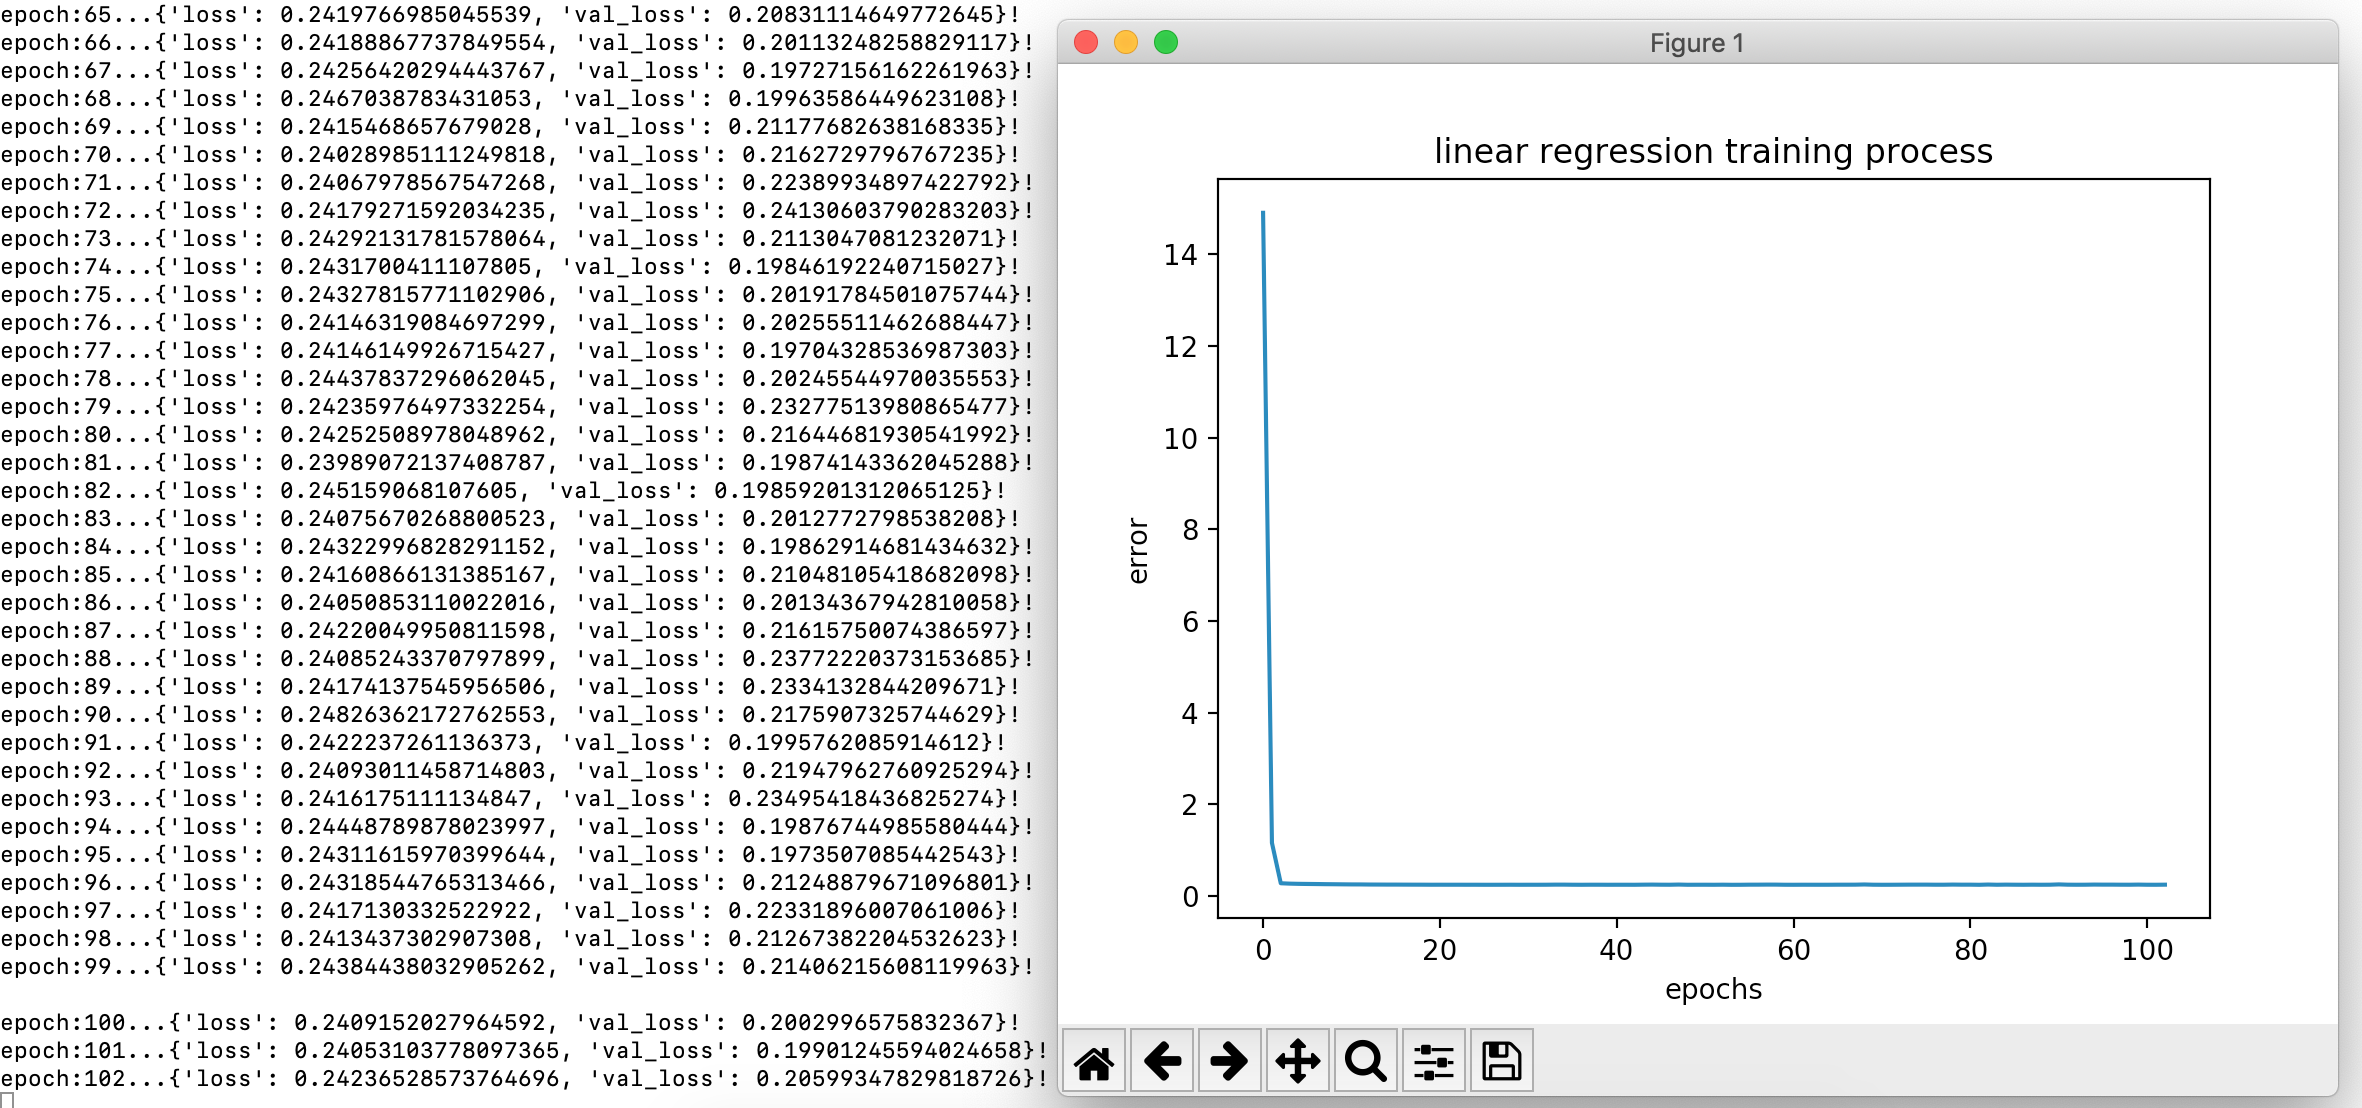
\includegraphics[height=5cm]{images/f000051}
\end{figure}
最后的协整信号结果:
\begin{figure}[H]
	\caption{协整信号}
	\label{f000052}
	\centering
	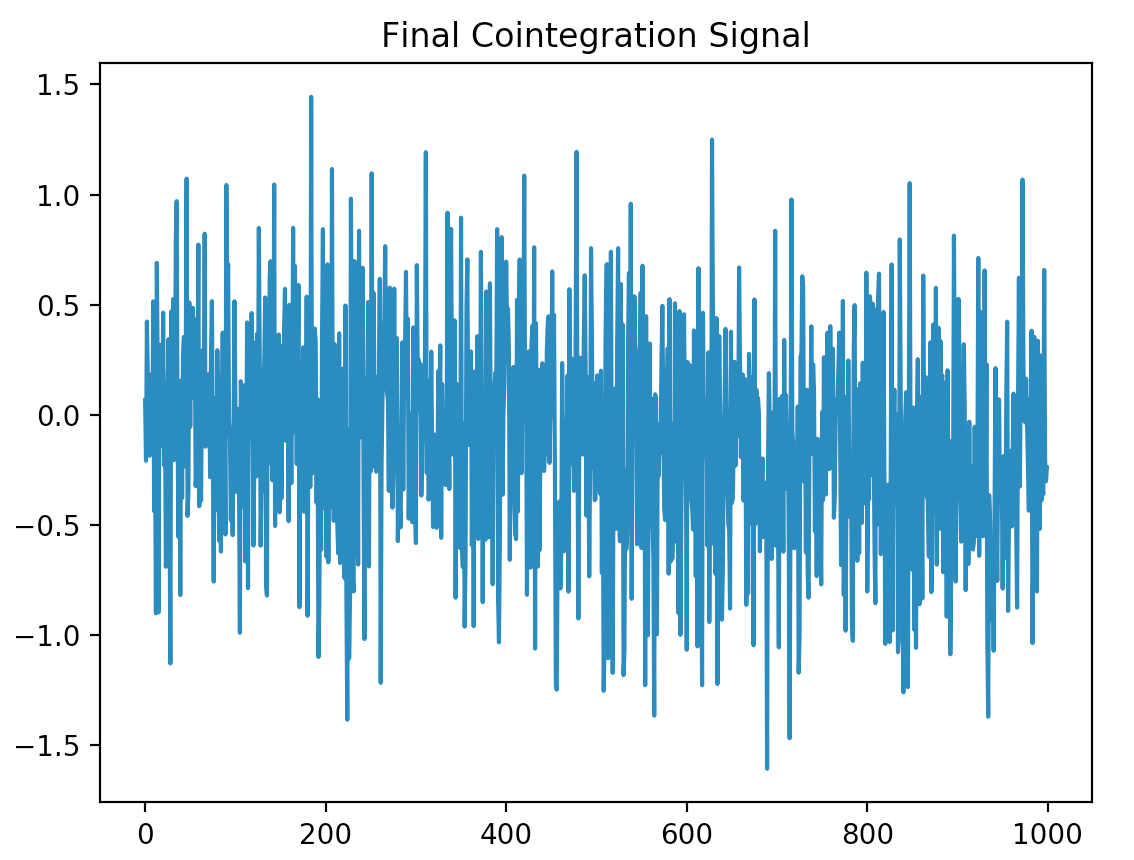
\includegraphics[height=5cm]{images/f000052}
\end{figure}
程序的运行结果如下所示:
\begin{figure}[H]
	\caption{程序运行结果}
	\label{f000053}
	\centering
	\includegraphics[height=5cm]{images/f000053}
\end{figure}
由于以y为自变量时ADF检验的p值较小,所以取以y为自变量的情况,计算出来的对冲比例为0.51,与实际值0.5非常接近,
这证明我们的算法是正确的。
\subsection{Johansen检验}
我们已经讲述了协整模型理论,可以比较好的处理两个交易对的对冲比例和均值回归的问题。但是这里面有两个问题,首先在协整模
型中,我们假设交易对中的两个标的是线性关系,其次我们只能处理有两个标的的交易对。在本节中,我们将根据\cite{r000001}
投资组合理论,处理标的之间不是线性关系,以及多个交易标的的均值回归策略研发问题。\newline
在实际应用中,我们经常用到的模型是Johansen Test模型,有时也叫VECM模型。在这一节中,我们将来讲解这个模型。Johansen模
型是基于向量自回归VAR模型的。我们以前所讲的自回归模型,都是标量的自回归模型,向量自回归模型定义为:
\begin{equation}
\boldsymbol{x}_{t} = \boldsymbol{\mu} + A_{1}\boldsymbol{x}_{t-1} + ... + A_{p}\boldsymbol{x}_{t-p} + \boldsymbol{w}_{t}
\label{e000063}
\end{equation}
式中$\symbol{\mu}$为序列的均值向量,$\boldsymbol{w}_t$为白噪声向量。接下来我们定义向量误差修正模块VECM(Vector Error Correction Model):
\begin{equation}
\Delta \boldsymbol{x}_{t}= \boldsymbol{\mu} + A \boldsymbol{x}_{t-1} + \Gamma _{1} \Delta \boldsymbol{x}_{t-1} + ... + \Gamma _{p} \Delta \boldsymbol{x}_{t-p} + \boldsymbol{w}_t
\label{e000064}
\end{equation}
其中A为系数矩阵,$\Gamma _{i}$是各滞后期的系数矩阵。我们对矩阵A进行特征值分解,阶数为$r$,分为以下两种情况:
\begin{itemize}
\item $r=0$:表明没有线性协整模型;
\item $r>0$:至少有$r+1$个序列存在协整关系;
\end{itemize}
在实际应用中,我们取出最大的特征值对应的特征向量,将其元素作为对应序列的协整系数。





\maketitle\begin{center}
\Large \textbf{第5章 卡尔曼滤波}
\end{center}
\begin{abstract}
到目前为止,我们所讨论的基于协整模型的交易对策略,有一个重要的假设,即交易对之间的协整系数是不变的。但是在实际应用中,这些协整系数可能会发生缓慢的改变,如果我们用固定值,可能不会取得最佳的应用效果。在本章中,我们将采用State Space Model来解决这一问题,具体业讲,就是利用卡尔曼滤波技术,将交易对的对冲比例视为系统不可见的状态,将交易对中标的的收益率作为可观察项,利用卡尔曼滤波器的滤波功能,通过不断增加的新观测数据,利用贝叶斯推理,使我们能够更加精准的估计系统不可见状态,在本例中就是交易对的对冲比例。实际上,交易对的对冲比例,不仅会发生缓慢的变化,有时因为监管、宏观经济、市场事件等原因,交易对的对冲比例还可能发生剧烈的变化,这就需要我们识别市场所处状态,识别出市场状态的改变,从而做出更加科学的决策,这部分内容将在下一章隐马可夫模型章节中介绍。aqt005.py
\end{abstract}
\section{卡尔曼滤波}
\subsection{State Space Model概述}
在State Space Model中,我们要研究的对象是环境,这里就是市场。环境会处于某种状态,而且环境所处的状态随着时间而改变。但是我们不能直接观测到环境,我们只能得到一些观察,我们希望通过观察来推测出系统年处的状态。以我们当前的任务为例,我们的环境就是市场上的交易对,而状态就是交易对的对冲比例,而由于各种原因,如市场微观结构等,我们只能得到交易对标的的收益率,其中具有很大的噪声,信噪比很低,我们的任务就是通过观察这些收益率数据,得到交易对的对冲比例。
State Space Model可以用如下图形来表示:
\begin{figure}[H]
	\caption{通用State Space Model}
	\label{f000054}
	\centering
	\includegraphics[height=10cm]{images/f000054}
\end{figure}
图中上面白色的圆圈代表环境的隐藏状态$x_{t}$,蓝色的圆圈代表环境的观测值$y_{t}$,系统会从一个状态转移到另一个状态,可以用一个概率$P(x_{t})x_{t-1}$来表示,环境所处状态决定观察值$P(y_{t} \vert x_{t})$,环境初始时的概率为$P(x_{0})$,根据这些变量的不同特性,我们可以把State Space Model分为四种类型:
\begin{table}[H]
\caption{State Space Model类型}
\label{t000001}
\begin{tabular}{|c|c|c|c|} \hline
名称 & $P(x_{t} \vert x_{t-1})$ & $P(y_{t} \vert x_{t})$ & $P(x_{0})$ \\ \hline  
离散模型(隐马可夫模型) & $A_{x_{t-1}, x_{t}}$ & Any & $\pi$ \\ \hline
线性高斯(卡尔曼滤波器) & $\mathcal{N}\big(  Ax_{t-1}+B, \theta \big)$ & $\mathcal{N}\big(  Hx_{t}+C, R \big)$ & $\mathcal{N}\big(  \mu _{0}, \epsilon _{0} \big)$ \\ \hline
非线性非高斯(粒子滤波器) & $f(x_{t})$ & $g(y_{t})$ & $f_{0}(x_{0})$\\ \hline
\end{tabular}
\end{table}
利用State Space Model可以做三件事情:
\begin{enumerate}
\item 预测:预测下一个到几个时刻的状态值;
\item 滤波:根据当前的观察值,预测系统状态;
\item 平滑:利用过去的观察值,解释过去状态变化情况;
\end{enumerate}
在这一章,我们所研究是线性高斯模型,即卡尔曼滤波器,我们同时会利用贝叶斯推断,通过不断增加的观察值,来逐步精确预测环境状态,在这里就是交易对的对冲比例。\newline
\subsection{数学原理}
在这一部分,我们将简单讲述卡尔曼滤波的数学原理,公式和符号会比较多,但是重点是理解其背后的数据直觉,不必纠结与具体推导过程。\newline
环境状态我们用一个向量来表示$\boldsymbol{x}_{t} \in R^{n}$,由于其会随时间变化,因此我们为其添加了下标$t$,因为卡尔曼滤波是线性高斯模型,当前时刻的状态,是由前一时刻的状态经线性组合再加上高斯噪声所组成,如下所示:
\begin{equation}
\boldsymbol{x}_{t} = A\boldsymbol{x}_{t-1} + \boldsymbol{b} + \boldsymbol{u}_{t}
\label{e000065}
\end{equation}
其中$A \in R{n \times n}$的矩阵,$\boldsymbol{b} \in R^{n}$,$\boldsymbol{w}_{t} \in R^{n}$为高斯白噪声。\newline
系统的观察用$\boldsymbol{y}_t \in R^{m}$表示,其由当前时刻环境状态的线性组合加高斯白噪声组成,如下所示:
\begin{equation}
\boldsymbol{y}_{t} = H\boldsymbol{x}_{t} + \boldsymbol{c} + \boldsymbol{v}_{r}
\label{e000066}
\end{equation}
系统初始状态为高斯分布:
\begin{equation}
\boldsymbol{x}_{0} \sim \mathcal{N} \big( \boldsymbol{\mu}_{0}, \Sigma _{0} \big)
\label{e000067}
\end{equation}
环境状态在t时刻噪声:
\begin{equation}
\boldsymbol{u}_{t} \sim \mathcal{N} \big( 0, \Sigma _{t}^{u} \big)
\label{e000068}
\end{equation}
环境观察在t时刻噪声:
\begin{equation}
\boldsymbol{v}_{t} \sim \mathcal{N} \big( 0, \Sigma _{t}^{v} \big)
\label{e000069}
\end{equation}
\subsection{PyKalman库介绍}
在这一节中,我们将讲述利用卡尔曼滤波来确定交易对的动态对冲比例。我们要研究的交易对为TLT和IEI,其面向美国债券市场,具有相同的市场因素,因此应该具有稳定的协整比例。在本节中我们将使用pykalman库,所以我们先来讲解一下在pykalman库中,卡尔曼滤波的表示方式,主要参考自\cite{r000003}。\newline
我们同样用$x_{t}$来代表环境的隐藏状态,用$y_{t}$来代表对环境的观察,则卡尔曼滤波可以表示为:
\begin{equation}
\boldsymbol{x}_{0} \sim \mathcal{N} \big( \boldsymbol{\mu}_{0}, \Sigma _{0} \big)
\label{e000070}
\end{equation}

\begin{equation}
\boldsymbol{x}_{t} = A_{t-1}\boldsymbol{x}_{t-1} + \boldsymbol{b}_{t-1} + \boldsymbol{\epsilon _{t}^{1}}
\label{e000071}
\end{equation}
\begin{equation}
\boldsymbol{y}_{t} = C_{t}\boldsymbol{x}_{t} + \boldsymbol{d}_{t} + \boldsymbol{\epsilon _{t}^{2}}
\label{e000072}
\end{equation}
\begin{equation}
\boldsymbol{\epsilon _{t}^{1}} \sim \mathcal{N} \big( 0, Q \big)
\label{e000073}
\end{equation}
\begin{equation}
\boldsymbol{\epsilon _{t}^{2}} \sim \mathcal{N} \big( 0, R \big)
\label{e000074}
\end{equation}
式中所用到符号如下所示:
\begin{table}[h]
\caption{PyKalman变量意义}
\label{t000002}
\begin{tabular}{|c|c|c|} \hline
表示 & 模型参数 & 意义 \\ \hline  
$\boldsymbol{\mu} _ {0}$ & initial\_state\_mean & 初始值均值向量 \\ \hline
$\Sigma _{0}$ & initial\_state\_covariance & 初始状态协方差矩阵 \\ \hline
A & transition\_matrices & 转移矩阵 \\ \hline
$\boldsymbol{b}$ & transition\_offsets &  转移偏置值 \\ \hline
Q & transition\_covariance & 转移协方差矩阵(噪声) \\ \hline
C & observation\_matrices & 观察矩阵 \\ \hline
$\boldsymbol{d}$ & observation\_offsets & 观察偏置值 \\ \hline
R & observation\_covariance & 观察协方差矩阵(噪声) \\ \hline
\end{tabular}
\end{table}
卡尔曼滤波中参数的估计是一个比较大的问题,我们可以通过EM()算法来根据现有的观察和环境状态数据,对参数进行估计。卡尔曼滤波的参数为:
\begin{equation}
\theta = \{A, \boldsymbol{b}, C, \boldsymbol{d}, Q, R, \boldsymbol{\mu}_{0}, \Sigma _{0}\}
\label{e000075}
\end{equation}
我们的目录是:
\begin{equation}
\arg \max _{\theta} P \big( \boldsymbol{y}_{0:T-1};\theta \big)
\label{e000076}
\end{equation}
具体算法比较复杂,作为应用开发者,我们只需要知道这可以通过PyKalman.em(observations)函数来实现就可以了。\newline
\subsection{卡尔曼滤波应用}
我们取到两个ETF的价格数据,并将其保存为文本文件,格式如下所示:
\begin{figure}[H]
	\caption{数据文件格式}
	\label{f000055}
	\centering
	\includegraphics[height=10cm]{images/f000055}
\end{figure}
卡尔曼滤波程序如下所示:
\lstset{language=PYTHON, caption={卡尔曼滤波示例}, label={c000014}}
\begin{lstlisting}
    def hedge_ratio(self):
        etfs = ['TLT', 'IEI']
        start_date = "2010-8-01"
        end_date = "2016-08-01"
        # 获取调整后的收盘价
        dateparse = lambda x: pd.datetime.strptime(x, '%Y-%m-%d')
        prices = pd.read_csv('./work/aqt005_001.txt', encoding='utf-8', parse_dates=['Date'], date_parser=dateparse, index_col='Date')
        # 画散点图
        self.draw_date_coloured_scatterplot(etfs, prices)
        state_means, state_covs = self.calc_slope_intercept_kalman(etfs, prices)
        self.draw_slope_intercept_changes(prices, state_means)
        
    def draw_date_coloured_scatterplot(self, etfs, prices):
        """
        生成散点图,以交易对中两个标的为坐标轴,可以直观观察两个标的间的关系,并且
        采用黄色代表早期数据而红色代表近期数据
        @param etfs 标的字符列表
        @param prices 价格列表,每行为日期、TLT价格、IEI价格
        """
        plen = len(prices)
        colour_map = plt.cm.get_cmap('YlOrRd')
        colours = np.linspace(0.1, 1, plen)
        # 生成散点图
        scatterplot = plt.scatter(
        prices[etfs[0]], prices[etfs[1]],
        s=30, c=colours, cmap=colour_map,
        edgecolor='k', alpha=0.8
        )
        # 添加颜色图表
        colourbar = plt.colorbar(scatterplot)
        colourbar.ax.set_yticklabels(
        [str(p.date()) for p in prices[::plen//9].index]
        )
        plt.xlabel(prices.columns[0])
        plt.ylabel(prices.columns[1])
        plt.show()
        
    def calc_slope_intercept_kalman(self, etfs, prices):
        """
        使用卡尔曼滤波器预测对冲比例
        """
        delta = 1e-5
        mu0 = np.zeros(2)
        sigma0 = np.ones((2, 2))
        Q = delta / (1 - delta) * np.eye(2)
        At = np.eye(2)
        Ct = np.vstack(
            [prices[etfs[0]], np.ones(prices[etfs[0]].shape)]
        ).T[:, np.newaxis]
        R = 1.0
        kf = KalmanFilter(
            n_dim_obs=1,
            n_dim_state=2,
            initial_state_mean=mu0,
            initial_state_covariance=sigma0,
            transition_matrices=At,
            observation_matrices=Ct,
            observation_covariance=R,
            transition_covariance=Q
        )
        
        yt = prices[etfs[1]].values
        #state_means, state_covs = kf.em(observations).filter(observations)
        xt_means, xt_covs = kf.em(yt).filter(yt)
        return xt_means, xt_covs
        
    def draw_slope_intercept_changes(self, prices, state_means):
        """
        绘制斜率和截距
        """
        pd.DataFrame(
            dict(
                slope=state_means[:, 0],
                intercept=state_means[:, 1]
            ), 
            index=prices.index
        ).plot(subplots=True)
        plt.show()
\end{lstlisting}
我们首先从数据文件中读出调整后的收盘价格数据,然后以TFT为横轴,IEI为纵轴,绘制出这两个标的间的对应关系。如下所示:
\begin{figure}[H]
	\caption{散点图}
	\label{f000056}
	\centering
	\includegraphics[height=10cm]{images/f000056}
\end{figure}
由图\ref{f000056}可以看出,二者之间有一个相对稳定的线性关系,这是我们应用交易对交易策略的基础。\newline
我们接着利用卡尔曼滤波来预测对冲比例,为了讲述方便,我们把PyKalman库中的公式重新列在这里:
\begin{equation}
\boldsymbol{x}_{t-1}=A_{t}\boldsymbol{x}_{t-1} + \boldsymbol{b}_{t} + \boldsymbol{\epsilon}_{t}^{1}
\label{e000077}
\end{equation}
\begin{equation}
\boldsymbol{y}_{t}=C_{t}\boldsymbol{x}_{t} + \boldsymbol{d}_{t} + \boldsymbol{\epsilon}_{t}^{2}
\label{e000078}
\end{equation}
\begin{equation}
\boldsymbol{\epsilon}_{t}^{1} \in \mathcal{N} \big( 0, Q \big)
\label{e000079}
\end{equation}
\begin{equation}
\boldsymbol{\epsilon}_{t}^{2} \in \mathcal{N} \big( 0, R \big)
\label{e000080}
\end{equation}
我们将TLT的价格,后面加上1之后形成向量,将当前所有时间点的向量组合到一起,形成的矩阵作为观察矩阵,即公式中的$C_{t}$。观察$y_{t}$在这里为1维,因此初始时其协方差矩阵为1。我们按照给定的初始初始化一个卡尔曼滤波器对象,首先调用em()方法对参数进行估计,然后利估计出的参数,运行滤波功能,得到本时刻系统状态即对冲比例。对于每个时间点,其公式为:
\begin{equation}
y_{t}=\begin{bmatrix}
c_{t} & 1
\end{bmatrix}\begin{bmatrix}
x_{t,1} \\
x_{t,2}
\end{bmatrix} \quad => \quad IEI.price=\begin{bmatrix}
TLT.price & 1
\end{bmatrix}\begin{bmatrix}
slope \\
intercept
\end{bmatrix}
\label{e000081}
\end{equation}
注意:在上式中,我们将截距项$\boldsymbol{d}_{t}$作为向量中的一维来表示,因此式中就没有这一项了。\newline
运行上面的程序,就可以得到各个时间点的斜率和截距,我们接着绘制斜率和截距随时变化的曲线,如下所示:
\begin{figure}[H]
	\caption{对冲比例变化曲线}
	\label{f000057}
	\centering
	\includegraphics[height=10cm]{images/f000057}
\end{figure}
图\ref{f000057}中,上面蓝色的曲线为对冲比例变化曲线,可以看出,对冲比例并不是一成不变的,因此如果我们按照动态变化的对冲比例来设计交易策略,我们可以得到更高的收益。

\maketitle\begin{center}
\Large \textbf{第6章 统计套利策略}
\end{center}
\begin{abstract}
在本章中,我们将利用卡尔曼滤波技术,设计统计套利策略,利用我们的量化交易研究平台进行回测,初步验证策略的正确性。
并将GARCH模型用于实际金融时间序列数据拟合。
\end{abstract}
\section{统计套利策略}
统计套利策略是一种市场中性策略,在实际中有大量应用。
\subsection{数据获取}
我们要研究交易策略,首先要获取历史交易数据,在本节中,我们将讲述如何通过baostock的接口,来获取历史交易数据。我们之所以选择baostock接口,因为baostock可以提供免费的6分钏的日内交易数据,这在免费数据中是很少见的。不过我们这一篇中,我们只研究日线交易数据。baostock接口网站:
\lstset{language=BASH}
\begin{lstlisting}
http://baostock.com/baostock/index.php
\end{lstlisting}
获取股票历史交易记录非常简单,甚至都不用注册用户,例如我们想获取工商银行2006到至2018年数据,根据baostock的规定,工商银行的股票代码为601398.sh,程序如下所示:
\lstset{language=PYTHON, caption={baostock获取股票历史行情数据}, label={c000015}}
\begin{lstlisting}
import baostock as bs
import pandas as pd

class BsCnaDaily(object):
    def __init__(self):
        self.name = 'BsADaily'
        
    def get_history_data(self, stock_code, start_date, end_date):
        '''
        获取A股日线行情历史数据
        @param stock_code 股票代码,如工商银行为:sh.601398
        @param start_date 开始日期,格式yyyy-MM-dd
        @param end_date 结束日期,格式yyyy-MM-dd
        @return 获取成功返回True,否则返回False
        @version v0.0.1 闫涛 2019-04-22
        '''
        lg = bs.login()
        if lg.error_code != '0':
            print('login respond  error_msg:'+lg.error_msg)
            return False, lg.error_msg
        rs = bs.query_history_k_data_plus(stock_code,
                "date,code,open,high,low,close,preclose,volume,amount,adjustflag,turn,tradestatus,pctChg,isST",
                start_date=start_date, end_date=end_date,
                frequency="d", adjustflag="3")
        if rs.error_code != '0':
            print('query_history_k_data_plus respond  error_msg:'+rs.error_msg)
            return False,rs.error_msg
        data_list = []
        while (rs.error_code == '0') & rs.next():
            data_list.append(rs.get_row_data())
        result = pd.DataFrame(data_list, columns=rs.fields)
        result.to_csv('./data/{0}.csv'.format(stock_code), index=False)
        bs.logout()
        return True
\end{lstlisting}
调用方法如下所示:
\lstset{language=PYTHON, caption={baostock获取股票历史行情数据示例}, label={c000016}}
\begin{lstlisting}
import csv
import pandas as pd
import matplotlib.pyplot as plt
from core.quotation.bs_cna_daily import BsCnaDaily

class TpsaDataset(object):
    def __init__(self):
        self.name = 'TpsaDataset'
        
    @staticmethod
    def get_quotation_data(stocks):
        '''
        获取交易对行情数据
        @params stocks np.array [0][...]和[1][...]分别代表交易对
            对于交易对:[0]{stock_code, start_date, end_date, eft_name}
            其中eft_name也是数据文件保存的名字,stocks共有两条记录,由
            调用者负责保证
        '''
        print(stocks[0]['stock_code'])
        bs_cna_daily = BsCnaDaily()
        # 工商银行(股票代码60开头的是上海)
        bs_cna_daily.get_history_data(stocks[0]['stock_code'], 
                    stocks[0]['start_date'], stocks[0]['end_date'], 
                    stocks[0]['etf_name'])
        bs_cna_daily.get_history_data(stocks[1]['stock_code'], 
                    stocks[1]['start_date'], stocks[1]['end_date'], 
                    stocks[1]['etf_name'])
            
    @staticmethod
    def draw_close_price_curve(stock_files):
        '''
        绘制股票收益率曲线
        @stock_files 交易对股票行情文件名,共有两个
        '''
        print('绘制收盘价曲线...')
        etf0_prices = TpsaDataset.read_close_prices(stock_files[0])
        etf1_prices = TpsaDataset.read_close_prices(stock_files[1])
        plt.title('close price curve')
        plt.plot(etf0_prices)
        plt.plot(etf1_prices)
        plt.show()
    
    @staticmethod
    def read_close_prices(stock_file):
        '''
        读取股票收盘价数据时间序列
        @param stock_file 股票行情文件
        @return 股票收盘价的list
        '''
        close_prices = []
        with open(stock_file, 'r', newline='') as fd:
            rows = csv.reader(fd)
            header = next(rows)
            print('header:{0}'.format(header))
            for row in rows:
                close_prices.append(float(row[4]))
        return close_prices
        
    @staticmethod
    def read_close_price_pd(stock_file):
        dateparse = lambda x: pd.datetime.strptime(x, '%Y-%m-%d')
        prices = pd.read_csv(stock_file, encoding='utf-8', 
                parse_dates=['Date'], date_parser=dateparse, 
                index_col='Date')
        print(prices.values[:, 3])
\end{lstlisting}
\subsection{卡尔曼滤波策略}
在本例中,我们将工商银行收盘价作为自变量,将建设银行收盘价作为因变量。按照卡尔曼滤波框架,我们将建设银行的收盘价视为可观测状态$y_{t}$,而建设银行收盘价与工商银行收盘价之比,包括斜率和截距,视为系统验证状态,将工商银行收盘价视为观测矩阵,这样就组成了一个卡尔滤波模型。系统在刚开始运行时,我们拿一部分历史数据运行卡尔曼滤波器,通过EM算法,估计出卡尔曼滤波器中的参数,之后再根据历史数据运行回测流程。\newline
我们首先运行kalman.filter方法,求出系统的状态,然后根据工商银行收盘价和filter方法返回的系统状态中的斜率和截距,求出建设银行的计算值,将建设银行计算值与建设银行收盘价真实值相减得天误差,然后将其与观察向量计算中的误差的标准差相比较,如果小于负的标准差,则买入建设银行股票,并按斜率比例卖出对应数量的工商银行股份;如果大于标准差,则卖出建设银行股票,并按斜率比例买入对应数量的工商银行股票。具体代码如下所示:
\lstset{language=PYTHON, caption={卡尔曼滤波协整模型交易对策略}, label={c000017}}
\begin{lstlisting}
from __future__ import print_function

from math import floor
import math

import numpy as np

from qstrader.price_parser import PriceParser
from qstrader.event import (SignalEvent, EventType)
from qstrader.strategy.base import AbstractStrategy
from pykalman import KalmanFilter


class TpsaStrategy(AbstractStrategy):
    """
    Requires:
    tickers - The list of ticker symbols
    events_queue - A handle to the system events queue
    """
    def __init__(
        self, tickers, events_queue, equity, ts0, ts1
    ):
        self.tickers = tickers
        self.events_queue = events_queue
        self.equity = equity
        self.time = None
        self.latest_prices = np.array([-1.0, -1.0])
        self.invested = None

        self.delta = 1e-4
        self.wt = self.delta / (1 - self.delta) * np.eye(2)
        self.vt = 1e-3
        self.theta = np.zeros(2)
        self.P = np.zeros((2, 2))
        self.R = None

        self.days = 0
        self.qty = 20000
        self.cur_hedge_qty = self.qty
        
        self.yt_state = 0
        self.buy_price = 0.0
        
        self.ts0 = ts0
        self.ts1 = ts1
        self.kalman_mode = 1
        
        xt_means, xt_covs = self.train_kalman_filter(ts0, ts1)
        slope = xt_means[-1][0]
        # 将80%资金按1:slope比例购买ts1和ts0
        price0 = ts0[-1]
        price1 = ts1[-1]
        print('type:{0}; shape:{1}'.format(type(price0), ts0[-1].shape))
        amount = self.equity * 0.1
        amount1 = amount / (1 + slope)
        amount0 = amount * (slope / (1+slope))
        self.qty1 = int(math.floor(amount1 / price1))
        self.qty1_0 = self.qty1
        self.qty0 = int(math.floor(amount0 / price0))
        self.qty0_0 = self.qty0
        amt1 = self.qty1 * price1
        amt0 = self.qty0 * price0
        self.equity -= (amt0 + amt1)
        self.equity_0 = self.equity
        self.events_queue.put(SignalEvent(self.tickers[0], "BOT", self.qty0))
        print('购买{0}:数量:{1};价格:{2}'.format(self.tickers[0], self.qty0, self.ts0[-1]))
        self.events_queue.put(SignalEvent(self.tickers[1], "BOT", self.qty1))
        print('购买{0}:数量:{1};价格:{2}'.format(self.tickers[1], self.qty1, self.ts1[-1]))
        print('现金:{0}'.format(self.equity))
        
        self.ts0 = np.array([])
        self.ts1 = np.array([])
        self.deltas = np.array([])
        
        

    def _set_correct_time_and_price(self, event):
        """
        Sets the correct price and event time for prices
        that arrive out of order in the events queue.
        """
        # Set the first instance of time
        if self.time is None:
            self.time = event.time
        
        # Set the correct latest prices depending upon 
        # order of arrival of market bar event
        price = event.adj_close_price/float(
            PriceParser.PRICE_MULTIPLIER
        )
        if event.time == self.time:
            if event.ticker == self.tickers[0]:
                self.latest_prices[0] = price
            else:
                self.latest_prices[1] = price
        else:
            self.time = event.time
            self.days += 1
            self.latest_prices = np.array([-1.0, -1.0])
            if event.ticker == self.tickers[0]:
                self.latest_prices[0] = price
            else:
                self.latest_prices[1] = price

    def train_kalman_filter(self, ts0, ts1, mode=1):
        """
        Utilise the Kalman Filter from the PyKalman package
        to calculate the slope and intercept of the regressed
        ETF prices.
        """
        delta = 1e-5
        mu0 = np.zeros(2)
        sigma0 = np.ones((2, 2))
        Q = delta / (1 - delta) * np.eye(2)
        At = np.eye(2)
        Ct = np.vstack(
            [ts0, np.ones(ts0.shape)]
        ).T[:, np.newaxis]
        R = 1.0
        self.kf = KalmanFilter(
            n_dim_obs=1,
            n_dim_state=2,
            initial_state_mean=mu0,
            initial_state_covariance=sigma0,
            transition_matrices=At,
            observation_matrices=Ct,
            observation_covariance=R,
            transition_covariance=Q
        )
        yt = ts1
        #state_means, state_covs = kf.em(observations).filter(observations)
        if mode != 1:
            xt_means, xt_covs = self.kf.filter(yt)
        else:
            xt_means, xt_covs = self.kf.em(yt).filter(yt)
        return xt_means, xt_covs


    def calculate_signals(self, event):
        mode = 2
        if event.type == EventType.BAR:
            self._set_correct_time_and_price(event)
            # Only trade if we have both observations
            if all(self.latest_prices > -1.0):
                # kalman.filter_update
                self.ts0 = np.append(self.ts0, self.latest_prices[0])
                self.ts1 = np.append(self.ts1, self.latest_prices[1])
                if self.days < 100:
                    return
                if self.days % 30 == 0:
                    mode = 1
                xt_means, x_convs = self.train_kalman_filter(self.ts0, self.ts1, mode=2)
                slope = xt_means[-1][0]
                intercept = xt_means[-1][1]
                yt_hat = self.ts0[-1] * slope + intercept
                delta = yt_hat - self.ts1[-1]
                self.deltas = np.append(self.deltas, delta)
                threshold = np.std(self.deltas)
                if delta < -threshold:
                    # 卖掉0买入1
                    qty0 = int(math.floor(self.qty * slope))
                    self.events_queue.put(SignalEvent(self.tickers[0], "SLD", qty0))
                    self.qty0 -= qty0
                    self.equity += qty0 * self.latest_prices[0]
                    self.events_queue.put(SignalEvent(self.tickers[1], "BOT", self.qty))
                    self.qty1 += self.qty
                    self.equity -= self.qty * self.latest_prices[1]
                    print('    买入{0}:数量:{1};价格:{2};金额:{3}'.format(
                            self.tickers[1], self.qty, self.latest_prices[1], 
                            self.qty*self.latest_prices[1])
                    )
                    print('     卖出{0}:数量:{1};价格:{2};金额:{3}'.format(
                            self.tickers[0], qty0, self.latest_prices[0],
                            qty0*self.latest_prices[0]
                    ))
                    total = self.equity + self.qty0 * self.latest_prices[0] + self.qty1 * self.latest_prices[1]
                    print('########### 总资产:{0}={1}+{2}+{2}'.format(total, self.equity, 
                            self.qty0 * self.latest_prices[0], self.qty1 * self.latest_prices[1]))
                elif delta > threshold:
                    # 买入0卖出1
                    self.events_queue.put(SignalEvent(self.tickers[1], "SLD", self.qty))
                    self.qty1 -= self.qty
                    self.equity += self.qty * self.latest_prices[1]
                    qty0 = int(math.floor(self.qty * slope))
                    self.events_queue.put(SignalEvent(self.tickers[0], "BOT", qty0))
                    self.qty0 += qty0
                    self.equity -= qty0 * self.latest_prices[0]
                    print('    买入{0}:数量:{1};价格:{2};金额:{3}'.format(
                            self.tickers[0], qty0, self.latest_prices[0], 
                            self.qty*self.latest_prices[0])
                    )
                    print('     卖出{0}:数量:{1};价格:{2};金额:{3}'.format(
                            self.tickers[1], self.qty, self.latest_prices[1],
                            qty0*self.latest_prices[1]
                    ))
                    total = self.equity + self.qty0 * self.latest_prices[0] + self.qty1 * self.latest_prices[1]
                    print('########### 总资产:{0}={1}+{2}+{2}'.format(total, self.equity, 
                            self.qty0 * self.latest_prices[0], self.qty1 * self.latest_prices[1]))
\end{lstlisting}
另外,在程序中需要注意的部分为我们每隔一定的交易日,会重新使用EM算法来估计卡尔曼滤波器的参数,这样可以使我们的估计更加准确。
\subsection{卡尔曼滤波引擎}
我们在策略引擎中,初始化策略,调用平台进行回测,统计回测效果,代码如下所示:
\lstset{language=PYTHON, caption={卡尔曼滤波策略引擎}, label={c000018}}
\begin{lstlisting}
import calendar
import datetime
import numpy as np
from qstrader import settings
from qstrader.strategy.base import AbstractStrategy
from qstrader.position_sizer.naive import NaivePositionSizer
from qstrader.event import SignalEvent, EventType
from qstrader.compat import queue
from qstrader.trading_session import TradingSession
from qstrader.price_handler.bscna_daily_csv_bar import BscnaDailyCsvBarPriceHandler

import matplotlib.pyplot as plt
from app.tpsa.tpsa_dataset import TpsaDataset



from app.tpsa.tpsa_strategy import TpsaStrategy

class TpsaEngine(object):
    def __init__(self):
        self.name = 'QhEngine'
        
    def startup(self):
        testing = False
        config = settings.load_config()
        tickers = ['ICBC', 'CBC']
        # 读取用于估计卡尔曼滤波参数的时间序列
        ts0 = np.array(TpsaDataset.read_close_prices('./data/{0}_train.csv'.format(tickers[0])))
        ts1 = np.array(TpsaDataset.read_close_prices('./data/{0}_train.csv'.format(tickers[1])))
        
        self.title = [
            '基于卡尔曼滤波器的交易对策略'
        ]
        self.initial_equity = 1000000.0
        self.start_date = datetime.datetime(2017, 1, 1)
        self.end_date = datetime.datetime(2019, 4, 23)
        # Use the Monthly Liquidate And Rebalance strategy
        self.events_queue = queue.Queue()
        self.strategy = TpsaStrategy(
            tickers, self.events_queue, self.initial_equity, ts0, ts1
        )
        self.run(config, testing, tickers) 

    def run(self, config, testing, tickers):
        # Use the Naive Position Sizer where
        # suggested quantities are followed
        position_sizer = NaivePositionSizer()
        # Set up the backtest
        backtest = TradingSession(
            config, self.strategy, tickers,
            self.initial_equity, self.start_date, self.end_date,
            self.events_queue, title=self.title,
            position_sizer=position_sizer,
            price_handler=BscnaDailyCsvBarPriceHandler(
                config.CSV_DATA_DIR, self.events_queue,
                tickers, start_date=self.start_date,
                end_date=self.end_date
            )
        )
        results = backtest.start_trading(testing=testing)
        print('最后金额:{0}'.format(self.strategy.equity))
        
        total = self.strategy.equity + self.strategy.qty0 * \
                self.strategy.latest_prices[0] + \
                self.strategy.qty1 * self.strategy.latest_prices[1]
        print('########### 总资产:{0}={1}+{2}+{3}'.format(
                total, self.strategy.equity, 
                self.strategy.qty0 * self.strategy.latest_prices[0], 
                self.strategy.qty1 * self.strategy.latest_prices[1]
        ))
        delta0 = self.strategy.qty0 - self.strategy.qty0_0
        amt0 = 0.0
        if delta0 > 0:
            amt0 = self.strategy.latest_prices[0] * delta0
        else:
            amt0 = -self.strategy.latest_prices[0] * delta0
        delta1 = self.strategy.qty1 - self.strategy.qty1_0
        amt1 = 0.0
        if delta1 > 0:
            amt1 = self.strategy.latest_prices[1] * delta1
        else:
            amt1 = -self.strategy.latest_prices[1] * delta1
            
        print('initial:{0} vs final {1}'.format(self.strategy.equity_0, self.strategy.equity+amt0+amt1))
        
        return results
        
    
    def prepare_data(self):
        stocks = [
            {
                'stock_code': 'sh.601398',
                'start_date': '2019-03-01',
                'end_date': '2019-04-29',
                'etf_name': 'ICBC'
            }, 
            {
                'stock_code': 'sh.601939',
                'start_date': '2019-03-01',
                'end_date': '2019-04-29',
                'etf_name': 'CBC'
            }
        ]
        TpsaDataset.get_quotation_data(stocks)
        stock_files = [
            './data/{0}.csv'.format(stocks[0]['etf_name']),
            './data/{0}.csv'.format(stocks[1]['etf_name'])
        ]
        TpsaDataset.draw_close_price_curve(stock_files)

\end{lstlisting}
\subsection{运行结果}
通过如下代码可以运行这个策略的回测:
\lstset{language=PYTHON, caption={运行卡尔曼滤波策略引擎}, label={c000019}}
\begin{lstlisting}
        tpsaEngine = TpsaEngine()
        tpsaEngine.startup()
\end{lstlisting}
运行程序后,得到累积收益率曲线如下所示:
\begin{figure}[H]
	\caption{累积收益率曲线}
	\label{f000058}
	\centering
	\includegraphics[height=10cm]{images/f000058}
\end{figure}
在图形中有一段收益率非常高,但是在那个时间段,由于我们采用的是统计套利策略,并不会处理暴涨暴跌的情况,因此这段行情并没有把握住。关于这一点我们将在下一节进行讨论。\newline
年化夏普比曲线:
\begin{figure}[H]
	\caption{年化夏普比曲线}
	\label{f000059}
	\centering
	\includegraphics[height=10cm]{images/f000059}
\end{figure}
策略最大回撤图如下所示:
\begin{figure}[H]
	\caption{策略最大回撤}
	\label{f000060}
	\centering
	\includegraphics[height=10cm]{images/f000060}
\end{figure}
由于我们没在最高点时抛出股票,因此最大回撤图形上显得有些差,但是最后效果上面来看,应该还能说得过去。\newline
月收益率曲线:
\begin{figure}[H]
	\caption{月收益率曲线}
	\label{f000061}
	\centering
	\includegraphics[height=10cm]{images/f000061}
\end{figure}
年化收益率:
\begin{figure}[H]
	\caption{年化收益率曲线}
	\label{f000062}
	\centering
	\includegraphics[height=10cm]{images/f000062}
\end{figure}
总体统计信息:
\begin{figure}[H]
	\caption{总体统计信息}
	\label{f000063}
	\centering
	\includegraphics[height=10cm]{images/f000063}
\end{figure}
由上图可以看出,夏普比为0.88,通常较好的交易策略夏比应该在1以上,所以本策略还不是一个特别好的策略。
策略最终结果如下所示:
\begin{figure}[H]
	\caption{最终结果}
	\label{f000064}
	\centering
	\includegraphics[height=1cm]{images/f000064}
\end{figure}
在这个策略中,我们假设我们会长期持有50000股工商银行和50000股建设银行,每次波动对冲时交易20000股,初始时我们流动资金是100万,不采用资金杠杆,在回测结束时,我们将工商银行和建设银行恢复回各50000股,然后计算流动资金。由结果可以看出,我们在持股情况未变化的情况下,流动资金变为138.86万,实现了38.86万的盈利。这证明我们的策略还是基本可行的。策略最终夏普比为0.9,也处于较为理想的数值区间。
\subsection{讨论}
虽然我们基于卡尔曼滤波的协整模型,实际表现还算中规中矩,是一个可接受的交易策略,但是毕竟我们希望得到更高的收益率,在这一节中我们就来分析一下,为什么我们的交易策略收益率不是特别高呢?\newline
首先,我们没有采用资金杠杆,因为我们知道,交易对之间的相对波动较小,交易所还会收取交易费和印花税等费用,因此即使判断正确,每一单的盈利也是非常小的。如果我们可以使用资金杠杆,通常统计套利策略资金杠杆可以达到3$\sim$5倍,这样我们的收益率就会提高到100\%以上(扣除杠杆利息),这就是一个相当不错的交易策略了。例如,LTCM专门做德国国债和意大利国债交易对的基金,其资金杠杆高达数万倍。当然,使用资金杠杆,在放大收益率的同时,也会放大风险,如果判断失误,损失将非常惨重。事实上,红极一时的LTCM基金,就是因为一个决策失误,导致资金链断裂,最终破产的。\newline
其次,基于协整模型的交易对策略,虽然是一种市场中性策略,但是在市场剧烈波动时,由于信号具有非平稳性,在此期间应该停止交易,这通常通过交易平台的风控模块来实现,但是我们这个策略中没有风控模块。下图是工商银行和建设银行收盘价走势曲线图:
\begin{figure}[H]
	\caption{工商银行(蓝)和建设银行(红)收盘价曲线}
	\label{f000065}
	\centering
	\includegraphics[height=5cm]{images/f000065}
\end{figure}
由图\ref{f000065}可以看出,二者收盘价走势非常具有一致性,因此作为协整模型的交易对是没有问题的。但是大家请注意,在我们进行回测中间,二者的股价都有一次暴涨和回调,在这种行情下,显然应该采取以跟踪短期趋势为主的程序化交易CPA策略,而本章中的策略,基本没有对这一过程进行特别处理,这显然是需要优化的。


\maketitle\begin{center}
\Large \textbf{第6章 隐马可夫模型}
\end{center}
\begin{abstract}
在本章中我们讲述State Space Model中的隐马可夫模型,并且将该模型用于识别市场所处状态。在下一章中,将以此技术为基础,开发程序化CPA策略。
\end{abstract}
\section{隐马可夫模型}
我们所要研究的金融市场,经常处于变化之中,尤其是受政府政策、宏观调控、业务管制和突发事件等影响,市场状态会发生突然地剧烈的变化,如果我们的策略不作调整,就会使我们遭受巨大的损失。因此,对这种市场机制(Market Regime)进行研究,尤其是识别和预测市场机制的转变,是成功的量化交易所必需的。\newline
我们前几章中对时序信号进行研究过程中,在介绍这些方法时,都在强调这些方法研究的对象是具有平稳性的时序信号。但是当市场机制发生变化时,会使时序信号的均值、方差、自相关性和协方差发生变化,会产生相关性变化、异方差、肥尾等现象,因此研究和预测市场机制变化规律对量化交易而言非常重要。\newline
我们将采用在统计时间序列研究中最重要的隐马可夫模型,来研究市场机制变化规律。这种理论认为,市场机制及其变化,是由内部不可见的过程决定的,其会决定当前的市场机制以及之后市场机制的转换,我们只能通过投资标的的收益率,来间接地观测和研究这一过程。
\subsection{马可夫模型}
马可夫模型是一种随机的状态空间模型,系统会随机的从一种状态切换到另一种状态,状态之间的转换概率只与前一时刻的状态有关,而与之前的状态无关,我们称之为马可夫性质。例如,我们在前面章节中研究的随机游走时间序列,就是一种典型的具有马可夫性质的过程。\newline
根据系统的自治性和系统状态是否完全可见,可以将马可夫模型分为四大类,如下所示:
\begin{table}[H]
\caption{马可夫模型分类}
\label{t000003}
\begin{tabular}{|c|c|c|} \hline
 & 完全可见 & 部分可见 \\ \hline  
自治 & 马可夫链 & 隐马可夫模型(HMM) \\ \hline
控制 & 马可夫决策过程(MDP) & 部分可见马可夫决策过程(POMDP) \\ \hline
\end{tabular}
\end{table}
在这里我们首先明确一个概念,就是系统的状态和观测。系统状态是指系统内部的一种状态,我们不一定能完全观测到。系统观测是我们能够看到的系统性质,是系统状态的间接反映,但是不一定与系统状态相同。这样说比较抽象,让我们来看一个例子,如下图所示:
\begin{figure}[H]
	\caption{系统状态}
	\label{f000066}
	\centering
	\includegraphics[height=6cm]{images/f000066}
\end{figure}
系统状态就是在远处有一只老虎。但是在有些情况下,我们是无法观测到这个系统状态的,例如下图:
\begin{figure}[H]
	\caption{系统状态和系统观测}
	\label{f000067}
	\centering
	\includegraphics[height=6cm]{images/f000067}
\end{figure}
在上图中,有一辆汽车挡在了老虎的前面,这时我们的观测是系统中有一辆汽车,而我们就无从知道汽车后面还有一只老虎了,因此我们就不能得到系统状态了。在实际应用中,这种状态比较常见,例如在机器人应用中,机器人就观测不到被碍障物遮挡的物体和自己背后的物体,同样在我们的金融应用中,我们也观测不到决定市场机制变化的内部过程。\newline
当系统是自治的,即我们不能改变系统状态,而且系统状态是完全可见的情形,我们称之为马可夫链(MC:Markov Chain)。大家所熟知的马可夫链蒙特卡洛算法,就是在贝叶斯推理计算中一种常用的算法。\newline
当系统还是完体自治的,即我们无法改变系统状态,但是我们只能观测到部分的系统状态,这就是本章将要研究隐马可夫模型。在这种模型中,我们无法直接观测到系统的状态和状态间的转换,我们只能观测系统的某些外在表现,系统内部状态影响系统的外在表现。系统状态具有马可夫属性,即状态间转换只取决于前一状态,与历史状态无关。但是我们对系统的观测,不一定要具有马可夫性质。隐马可夫模型,除了在量化交易领域得到广泛应用外,在语音识别领域也得到了广泛的应用\newline
如果我们即Agent可以通过行动Action来影响系统状态,同时我们可以完全观测到系统的状态,这就是马可夫决策过程(MDP),又称为强化学习(RL:Reinforcement Learning)。这是当前人工智能三大方向之一,前两年大火的Alpha Go/Alpha Zero等,就是基于这种技术。我们会在最后一章中,详细讲解深度强化学习(DRL:Deep Reinforcement Learning)技术在量化交易中的应用。\newline
如果Agent可以通过行动Action来影响系统状态,但是只能间接观测到系统状态的外在表现,这就是部分可见马可夫决策过程(POMDP)。这部分是当前最前沿的研究方向,目前还没有特别成熟有效的解决方案。
\subsection{马可夫模型数学原理}
我们假设有一系列的观察值:$\{ X_{1}, X_{2}, ..., X_{t},...,X_{T} \}$,我们假设我们可以完全观测到系统的状态,因此$X_{t}$同时也是系统状态。同时,我们假设在任意时刻,我们的观测值$X_{t}$包含所有的信息,使我们能够预测出未来系统的状态。这一假设可以表示为如下的概率模型:
\begin{equation}
p(X_{1:T})= p(X_{1})p(X_{2} \vert X_{1})......p(X_{T} \vert X_{T-1})=p(X_{1})\prod_{t=2}^{T} p(X_{t} \vert X_{t-1})
\label{e000082}
\end{equation}
我们将$p(X_{t} \vert X_{t-1})$是$t-1$到$t$时刻的转移函数,同时转移概率与时间无关。\newline
我们假设有K个不同的状态,在$t-1$时刻处于状态$i$,在$t$时刻处于状态$j$,其转移概率为:
\begin{equation}
A_{i,j} = p(X_{t}=j \vert X_{t-1}=i)
\label{e000083}
\end{equation}
为简化问题,我们假设系统仅有两个状态,分别为1和2,在每个时刻,系统都处于这两个状态中的一个,系统从一个状态转移到另一个状态服从概率分布,并且与时间无关,我们可以通过下图来表示:
\begin{figure}[H]
	\caption{状态转移概率图}
	\label{f000068}
	\centering
	\includegraphics[height=6cm]{images/f000068}
\end{figure}
如图\ref{f000068}所示,当前时刻系统处在状态1,那么下一时刻还是状态1的概率为a,下一时刻为状态2的概率为1-a;如果当前时刻系统处在状态2,那么下一时刻还在状态2的概率为b,转移到状态1的概率为1-b,通常我们可以用状态转移矩阵来表示:
\begin{equation}
A = \begin{bmatrix}
1-\alpha & \alpha \\
\beta & 1 - \beta
\end{bmatrix}
\label{e000084}
\end{equation}
\subsection{隐马可夫模型数学原理}
如果我们不能完全观测到系统的状态,这时我们研究的问题就是隐马可夫模型。以我们本章要研究的问题为例,系统目前的市场机制对我们来说是不可见的,我们只能看到收益率,我们的任务就是根据收益率的变化情况,来推测系统所处的市场机制。\newline
我们假设系统共有K个状态,例如本章所研究的问题,我们可以认为K=3,分别对应为震荡、上涨、下跌,则系统状态用$z_{k},k \in \{1,..., K\}$来表示,系统观测用$x_{t}$来表示,系统状态可以决定系统观测,我们用$p(x_{t} \vert z_{t})$来表示。在隐马可夫模型中,系统处于某一个特定的状态,然后会突然转换到另一个新的状态,这与金融市场通常处于一种行情,突然发生一个突发事件,系统就从一种行情转换到另一种行情,是非常相似的,因此我们用隐马可夫模型来研究这一问题是非常适合的。
从$t=1$到$t=T$时刻,系统状态出现的概率为:
\begin{equation}
p(z_{1:T}) = p(z_{1}) \prod_{t=2}^{T}p(z_{t} \vert z_{t-1})
\label{e000085}
\end{equation}
系统观测出来的概率为:
\begin{equation}
p(x_{1:T} \vert z_{1:T}) = \prod_{t=1}^{T} p(x_{t} \vert z_{t})
\label{e000086}
\end{equation}
则根据观测值推断系统所处状态的概率表示为:
\begin{equation}
p(z_{1:T} \vert x_{1:T}) = p(z_{1:T}) p(x_{1:T} \vert z_{1:T}) = \bigg[ p(z_{1}) \prod_{t=2}^{T}p(z_{t} \vert z_{t-1}) \bigg] \bigg[ \prod_{t=1}^{T} p(x_{t} \vert z_{t}) \bigg]
\label{e000087}
\end{equation}
如果将这个模型应用于我们本章研究的问题,细心的读者可能就会有疑问,在上面的隐马可夫模型中,无论观测值还是系统状态,都是离散变量,而我们的所研究的问题中,股票的收益率为连续值,式\ref{e000087}中的$p(x_{t} \vert z_{t})$怎么计算呢?在实际应用中,我们假设在t时刻系统所处状态为k,即$z_{t}=k$,此时我们可以假设$x_{t}$服从如下所示的高斯分布:
\begin{equation}
x_{t} \sim \mathcal{N}(\mu _{k}, \sigma _{k}^{2})
\label{e000088}
\end{equation}
则有下式成立:
\begin{equation}
p(x_{t} \vert z_{t}=k; \theta) = \mathcal{N} (x_{t} \vert \mu _{k}, \sigma _{k}^{2})
\label{e000089}
\end{equation}
隐马可夫过程可以表示为如下所示形式:
\begin{figure}[H]
	\caption{隐马可夫模型示意图}
	\label{f000069}
	\centering
	\includegraphics[height=6cm]{images/f000069}
\end{figure}
隐马可夫模型可以实现三大任务:
\begin{itemize}
\item 预测:预测接下来的状态值;
\item 滤波:从观测序列预测当前状态值;
\item 平滑:从观测序列解释过去的状态值;
\end{itemize}
我们本章研究的任务是通过股票收益率变化曲线,预测市场所处状态,因此属于典型的滤波应用。\newline
在介绍了隐马可夫模型的基本理论之后,我们将以工商银行股票为例,讲解基于隐马可夫过程的程序化交易CPA策略。

\maketitle\begin{center}
\Large \textbf{第8章 程序化交易CPA策略}
\end{center}
\begin{abstract}
本章将通过隐马可夫模型来识别市场所处状态,在暴涨状态下买入对应股票,在暴跌状态下卖出对应股票,实现低买高卖,从而获得盈利。
\end{abstract}
\section{程序化交易CPA策略}
程序化交易CPA是一种短期趋势跟踪策略,通过汉斯123、布林带通道、MACD等技术分析手段,识别股票的涨跌趋势,实现低买高卖的策略。这种策略在市场行情剧烈波动,有大涨大跌行情时,可以实现相当可观的盈利。但是这种策略买卖的时间点非常重要,如果发现预测有误,就必须坚决的止损离场。所以有可能出现10次中9次因为趋势判断失误而止损离场,但是赚的一次所得的利润远远大于其余9次的亏损。\newline
在本章中,我们试图采用上一章中介绍的隐马可夫模型,来预测市场处于上涨行情、下跌行情还是震荡行情,在上涨行情时买入股票,在下跌行情时卖出股票,在震荡行情中停止交易。
\subsection{隐马可夫模型python实现}
在这一节中,我们利用hmmlearn库,来实现隐马可夫模型。
\subsubsection{求收益率}
我们第一步是根据工商银行股票的收盘价,计算出股票的收益率并绘制出收益率曲线:







\maketitle\begin{center}
\Large \textbf{第8章 集成策略}
\end{center}
\begin{abstract}
在本章中我们将基于卡尔曼滤波的协整模型策略与基于隐马可夫模型的程序化交易CPA策略相结合,在市场振荡期采用卡尔曼滤波模型,在暴涨暴跌期间,采用基于隐马可夫模型的程序化交易CPA策略,并与之前的策略进行比较。
\end{abstract}
\section{集成策略}


























\maketitle\begin{center}
\Large \textbf{第8章 机器学习}
\end{center}
\begin{abstract}
在本章中我们将首先讲述条件异方差模型GARCH(Generalized AutoRegressive Conditional Heteroskedastic),
并将GARCH模型用于实际金融时间序列数据拟合。aqt002.py
\end{abstract}
\section{机器学习}

\maketitle\begin{center}
\Large \textbf{第9章 高频日内交易}
\end{center}
\begin{abstract}
在本章中我们将首先讲述条件异方差模型GARCH(Generalized AutoRegressive Conditional Heteroskedastic),
并将GARCH模型用于实际金融时间序列数据拟合。aqt002.py
\end{abstract}
\section{高频日内交易}

\maketitle\begin{center}
\Large \textbf{第10章 长短时记忆网络}
\end{center}
\begin{abstract}
在本章中我们将首先讲述条件异方差模型GARCH(Generalized AutoRegressive Conditional Heteroskedastic),
并将GARCH模型用于实际金融时间序列数据拟合。aqt002.py
\end{abstract}
\section{长短时记忆网络(LSTM)}

\maketitle\begin{center}
\Large \textbf{第100章 \quad Transformer网络}
\end{center}
\begin{abstract}
在本章中我们将首先讲述去年年未在自然语言处理NLP中最流行的架构Transformer,然后介绍Transformer在股价预测方面的应用,接着利用TensorFlow Serving搭建策略服务,我们将该策略服务放到回测平台上进行测试,最后在实盘模拟平台上进行模拟交易。app/tqp
\end{abstract}
\section{Transformer网络}
\subsection{Transformer框架}
\subsection{Transformer量化应用}
\subsubsection{搭建colab开发环境}
\paragraph{配置Github}
首先到$https://www.puttygen.com/$网站下载puttygen的windows版本,用于生成访问github项目的公钥和私钥。以管理员身份运行puttygen.exe,点击界面中的"Generate":
\begin{figure}[H]
	\caption{生成公钥和私钥对}
	\label{f000040}
	\centering
	\includegraphics[height=2cm]{images/f000040}
\end{figure}
在图中的密码为"123456",点击保存私钥,将其保存到F:/docs/aqp\_github.ppk文件中。\newline
登录https://github.com/yt7589/aqp,在settings=>deploy keys中添加新的Key,将图\ref{f000040}中Public Key框中内容拷贝到下面的文本框中,如下所示:
\begin{figure}[H]
	\caption{将公钥添加到github中}
	\label{f000041}
	\centering
	\includegraphics[height=2cm]{images/f000041}
\end{figure}
接下来在Google colab中创建aqp.ipynb项目,添加代码单元格:
\lstset{language=PYTHON, caption={初始化github私钥}, label={c000010}}
\begin{lstlisting}
key = \
'''
PuTTY-User-Key-File-2: ssh-rsa
Encryption: aes256-cbc
Comment: rsa-key-20190411
Public-Lines: 6
AAAAB3NzaC1yc2EAAAABJQAAAQEAgWDxZNQtkqfNPnP1rHHIXx+Wi2HUL35RzXfo
T21fc+/gxjOQ7zG+V/KkTY0ZSuZBrdGhKRosamrBsaR+PrC3pqLNhOlFdUhsxvMg
YaLM79KUiirFp3dLHOqud4tuWE+BybsYmJA0m7sBJ6aUNXEoX8h5Nxy9VfHzfRIP
0ekeAA6vkd2PA5jy7AsbFCW1mwmBcu0ptAu3+sjLeIspsa0ED3vivUsnMeWQ87ll
DH7h3SC7InUlZLqr/gVKBrPnDSecAhVTTaoUG6PtTF0UkYYXixs1+daSBtEV568n
rRNV2cUkYseMnKwHdccXV2iVraHd11WsxJr2UDNt5nkKcpUkoQ==
Private-Lines: 14
qBX9VNU5GZoUAPvntTt8IRI7YqXfVgmKNVWDeyRFRGBlBsMVsU/o1AEm2pO9plHz
6vAuIje1fg70kDXcBuRCBiEJZ8IDdkNR5nqcgSFEnn2e/5UpisrA4FmGD99sSmWl
XJQAUEw5d7rxpQukiF6H19cJI+9e5vj9WIIKrCCXDawJyKaMQw0nn1zMJHsv6o21
MFlZqD8UUP4eoYrzRk2ga99O99b1MdYIwo2dUR40RQUGshKqIKdLHyiSBuy3gQm1
bmHNyrdMqCAN/88wadQRZvuyRudVXQAGbgYvDgZZV00EbiSOKPpmneK6DvgPaXea
J/1F+wAoZY8LsXZWlP2o44DjeJNmtc9eVPoR4b/hrG5fyMt9OmnCmL6Te6yue59L
pjH1gyvIMuoo3La71y8mlLKH8Hnb+bM5z6Ew7f/oMXzP9fNEdIsDN11L4WY9Gju1
GY0TUzi4h4li4K4Khzx1lOPDyaJahArx5iobD5xbemb4kj4OMRdsuQDqD7g32zVo
e8vVMgv8j3bzIpCAYmAmVhxslcpiFEUwjRtR6eyz7OL7g9IpkeG5fezGYMOLXxko
A1SWbIwqfODQhPJA1Pj3vnys8XVeQU04hplqyn955bwxl4abhVR3Q05E7DMYfdrR
f+a2VI4tAoWi7LCgskDnZ5754P3mUFkxSbILLt6tW+1Y4jbmPj6tP8GUI3Dm3zK6
qQAGkp3U9QeYlwsbO8lkTuWcW+NEyTfekjxnLtt1KLZufsKRDD1Dk4vQiXjKRCOU
UgjZ2Uui24d6N6ug/uiVNuxrDuZbpWpp2SYZEiuQCNhu3br+Q/+ZEZsmgslLewnr
ocK3qv7FUKq/Jg1QrjOmLq/RF1hVr+XcXzubiDcEdmZpFzsn7/VKHk/Jvv4f6IOd
Private-MAC: e16aabf8a23afa92f89fdeb3f5b2d36c20afb0ff

'''
! mkdir -p /root/.ssh
with open(r'/root/.ssh/id_rsa', 'w', encoding='utf8') as fh:
    fh.write(key)
! chmod 600 /root/.ssh/id_rsa
! ssh-keyscan gitlab.com >> /root/.ssh/known_hosts
\end{lstlisting}
在上面的代码中,先取出私钥文件中的内容,然后创建/root/.ssh目录,将私钥内容保存到/root/.ssh/id\_rsa文件中。运行上面的代码单元格,如果不报错就证明可以运行成功了。
\paragraph{下载源码文件}
可以通过如下命令获取github上的源码:
\lstset{language=BASH}
\begin{lstlisting}
!git clone https://github.com/yt7589/aqp.git
\end{lstlisting}
\paragraph{配置Google Drive文件系统}
我们需要读取保存在Google Drive中的数据集文件,因此我们需要建立一些特别工具来完成下面的内容。我们首先初始化环境:
\lstset{language=PYTHON, caption={初始化环境}, label={c000011}}
\begin{lstlisting}
from google.colab import drive
drive.mount('/content/drive')
\end{lstlisting}
这时需要访问提示中的网站,同意授权,将页面中授权码拷贝,将授权码粘贴到编辑框中并回车,然后我们就可像使用正常的目录一样来读写文件了。
\lstset{language=PYTHON, caption={初始化环境}, label={c000012}}
\begin{lstlisting}
with open('/content/drive/My Drive/fbm/README.md', 'r') as fd:
  readme = fd.read()
  print(readme)
\end{lstlisting}
其中fbm/是我们在Google Drive中创建的目录,使用这种方法,也不会出现中文乱码的问题。
具体用Transformer来预测股票价格的代码,colab的地址为:
\lstset{language=BASH}
\begin{lstlisting}
https://colab.research.google.com/drive/1PVwlbHfrndFhnNIjSLWaD1bsr-5olV1d#scrollTo=7s5HTXF9xall。
参考:
\lstset{language=BASH}
\begin{lstlisting}
https://github.com/llSourcell/Make_Money_with_Tensorflow_2.0/issues
\end{lstlisting}
\subsection{tqp平台}
\subsection{策略回测}
\subsection{实盘模拟}

\maketitle\begin{center}
\Large \textbf{第10章 深度强化学习}
\end{center}
\begin{abstract}
我们将市场看作是环境,买卖股票是Action,市场行情数据是Observation,经过长短时记忆网络(LSTM)或Transformer网络处理后形成State,盈利或亏损作为Reward,这样就组成了一个深度强化学习系统。在本章中,我们将研究基于深度强化学习的量化交易策略。
\end{abstract}
\section{深度强化学习}
\subsection{指数平滑技术}
在这一节中,我们将根据\cite{r000004}中所述的方法,讲述考虑到时序信号的趋势、周期等因素后的预测方法。
\subsubsection{指数平滑定义}
对于时间序列而言,我们需要分析出其趋势(涨、跌)和周期性变化。我们在这一节中,将采用Holt Winter方法来研究这一问题。\newline
给定一个时间序列,我们可以用这个序列的平均值来预测下一个值,如下所示:
\begin{equation}
\hat{y}_{T+1}=\frac{1}{T}\sum_{t=1}^{T}y_{t}
\label{e000091}
\end{equation}
代码如下所示:
\lstset{language=PYTHON, caption={利用序列平均值预测}, label={c000010}}
\begin{lstlisting}
    def predict_by_mean(self):
        y = np.array([3,10,12,13,12,10,12])
        return np.mean(y)
\end{lstlisting}
将整个序列的平均值作为下一个时间点的预测,显然有些问题,因为越往前的时间点对下一个时间点值的影响越小,所以在实际中我们通常使用移动平均的方法。我们首先设定移动窗口的大小W,其中前面各个时间点分配不同的权重$w_{i}$,例如我们假设移动窗口大小为4,其取值为:$[0.1, 0.2, 0.3, 0.4]$,越接近的时间点权值越大,利定数学语言表示为:
\begin{equation}
\hat{y}_{T+1}=\sum_{t=1}^{W}y_{t} \cdot w_{t}
\label{e000092}
\end{equation}
程序实现如下所示:
\lstset{language=PYTHON, caption={利用移动平均值预测}, label={c000011}}
\begin{lstlisting}
    def predict_by_mean(self):
        y = np.array([3,10,12,13,12,10,12])
        return np.mean(y)
\end{lstlisting}
在介绍了简单的移动平均概念之后,我们来介绍这一节的重点内容,指数平滑技术。$k$阶指数平滑的定义如下所示:
\begin{equation}
\hat{y}_{t}=\alpha \cdot y_{t} + \alpha (1-\alpha) y_{t-1} + \alpha (1-\alpha)^{2}y_{t-2} + ... + \alpha (1-\alpha)^{K} y_{t-K}=\sum_{i=1}^{K}\alpha(1-\alpha)^{k} y_{t-k}
\label{e000093}
\end{equation}
程序实现如下所示:
\lstset{language=PYTHON, caption={指数平滑实现}, label={c000012}}
\begin{lstlisting}
    def expopential_smoothing(self, series, alpha):
        result = [series[0]]
        for t in range(1, len(series)):
            result.append(alpha * series[t] + (1 - alpha) * result[t-1])
        return result
        
    def test_expopential_smoothing_3(self):
        holt_winters = HoltWinters()
        series = [3.0, 10.0, 12.0, 13.0, 12.0, 10.0, 12.0]
        alpha = 0.1
        r1 = holt_winters.expopential_smoothing(series, alpha)
        alpha = 0.9
        r2 = holt_winters.expopential_smoothing(series, alpha)
        
        fig, ax = plt.subplots()
        
        ax.plot(series, label='series')
        ax.plot(r1, label='a=0.1')
        ax.plot(r2, label='a=0.9')
        
        legend = ax.legend(loc='lower right', shadow=True, fontsize='medium')
        plt.show()        
\end{lstlisting}
绘制出的指数平滑图如下所示:
\begin{figure}[H]
	\caption{指数平滑示意图}
	\label{f000070}
	\centering
	\includegraphics[height=10cm]{images/f000070}
\end{figure}
图中蓝色曲线为真实序列,绿色曲线为$\alpha=0.9$时的平滑曲线,黄色曲线为$\alpha=0.1$时的平滑曲线。由上图可以看出$\alpha=0.9$时指数平滑的效果是最好的,如果选择合适的$\alpha$的过程我们称之为拟合,我们将在后面介绍。
\subsubsection{趋势周期预测}
在预测中,期望值又可以称为Level,用$\ell$表示。时序信号尤其是股票等信号,经常会有上涨或下跌趋势,我们可以用趋势来定义。在几何中,我们用如下公式定义斜率:
\begin{equation}
k=\frac{\Delta y}{\Delta x}
\label{e000094}
\end{equation}
因为对于时序信号来说,$\Delta x$通常代表一个时间单位,其值为1,所以斜率就是$\Delta y$,所以我们定义在$t$时刻的趋势为:
\begin{equation}
b_{t}=y_{t}-y_{t-1}
\label{e000095}
\end{equation}
大加入Level和趋势后,我们可以得出如下的双指数平滑公式:
Level的公式为:
\begin{equation}
\ell _{t} = \alpha y_{t} + (1-\alpha)(y_{t-1} + b_{t-1})
\label{e000096}
\end{equation}
趋势预测公式为:
\begin{equation}
b_{t} = \beta (\ell _{t} - \ell _{t-1}) + (1-\beta)b_{t-1}
\label{e000097}
\end{equation}
实际预测值为:
\begin{equation}
\hat{y}_{t}=\ell _{t} + b_{t}
\label{e000098}
\end{equation}
可以采用如下程序来实现上述算法:
\lstset{language=PYTHON, caption={趋势预测法}, label={c000013}}
\begin{lstlisting}
    def double_exponential_smoothing(self, series, alpha, beta):
        result = [series[0]]
        for n in range(1, len(series)+1):
            if n == 1:
                level, trend = series[0], series[1] - series[0]
            if n >= len(series): # we are forecasting
              value = result[-1]
            else:
              value = series[n]
            last_level, level = level, alpha*value + (1-alpha)*(level+trend)
            trend = beta*(level-last_level) + (1-beta)*trend
            result.append(level+trend)
        return result
        
    def test_double_expopential_smoothing(self):
        holt_winters = HoltWinters()
        series = [3.0, 10.0, 12.0, 13.0, 12.0, 10.0, 12.0]
        alpha = 0.9
        beta = 0.9
        result = holt_winters.double_exponential_smoothing(series, alpha, beta)
        
        fig, ax = plt.subplots()
        
        ax.plot(series, label='series')
        ax.plot(result, label='predict')
        
        legend = ax.legend(loc='lower right', shadow=True, fontsize='medium')
        plt.show()        
\end{lstlisting}
运行结果如下图所示:
\begin{figure}[H]
	\caption{趋势预测法}
	\label{f000071}
	\centering
	\includegraphics[height=10cm]{images/f000071}
\end{figure}
时序信号除了具有涨跌趋势规律之外,还可能具有周期性,例如一些信号随季节改变,因为我们还可以进一步将周期性变化考虑在内。我们假设时序信号的周期为L,即每过L个时间点就会重复。\newline
加入周期性后,我们的预测公式如下所示:
Level的公式为:
\begin{equation}
\ell _{t} = \alpha y_{t} + (1-\alpha)(y_{t-1} + b_{t-1})
\label{e000099}
\end{equation}
趋势预测公式为:
\begin{equation}
b_{t} = \beta (\ell _{t} - \ell _{t-1}) + (1-\beta)b_{t-1}
\label{e000100}
\end{equation}
周期预测公式:
\begin{equation}
s_{t} = \gamma (y_{t} - \ell _{t}) + (1-\gamma)s_{t-L}
\label{e000101}
\end{equation}
实际预测值为:
\begin{equation}
\hat{y}_{t+m}=\ell _{t} + mb_{t} + s_{t-L+1+(t-1)\%L}
\label{e000102}
\end{equation}
我们的初始趋势计算公式为:
\begin{equation}
b_{0}=\frac{1}{L} +\bigg(  \frac{y_{L+1}-y_{1}}{L} + \frac{y_{L+2}-y_{2}}{L} + ... + \frac{y_{L+L}-y_{L}}{L} \bigg)
\label{e000103}
\end{equation}
程序实现如下所示:
\lstset{language=PYTHON, caption={初始趋势计算}, label={c000014}}
\begin{lstlisting}
    def initial_trend(self, series, slen):
        sum = 0.0
        for i in range(slen):
            sum += float(series[i+slen] - series[i]) / slen
        return sum / slen
        
    def test_initial_trend(self):
        series = [30,21,29,31,40,48,53,47,37,39,31,29,17,9,20,24,27,35,41,38,
          27,31,27,26,21,13,21,18,33,35,40,36,22,24,21,20,17,14,17,19,
          26,29,40,31,20,24,18,26,17,9,17,21,28,32,46,33,23,28,22,27,
          18,8,17,21,31,34,44,38,31,30,26,32]
        holt_winters = HoltWinters()
        L = 12
        result = holt_winters.initial_trend(series, L)
        print(result) # 正确结果:-0.7847222222222222
        fig, ax = plt.subplots()
        
        ax.plot(series, label='series')
        
        legend = ax.legend(loc='lower right', shadow=True, fontsize='medium')
        plt.show()
        self.assertTrue(True)        
\end{lstlisting}
初始周期计算如下所示:
\lstset{language=PYTHON, caption={初始周期计算}, label={c000015}}
\begin{lstlisting}
    def initial_seasonal_components(self, series, slen):
        seasonals = {}
        season_averages = []
        n_seasons = int(len(series)/slen)
        # compute season averages
        for j in range(n_seasons):
            season_averages.append(sum(series[slen*j:slen*j+slen])/float(slen))
        # compute initial values
        for i in range(slen):
            sum_of_vals_over_avg = 0.0
            for j in range(n_seasons):
                sum_of_vals_over_avg += series[slen*j+i]-season_averages[j]
            seasonals[i] = sum_of_vals_over_avg/n_seasons
        return seasonals
        
    def test_initial_seasonal_components(self):
        series = [30,21,29,31,40,48,53,47,37,39,31,29,17,9,20,24,27,35,41,38,
          27,31,27,26,21,13,21,18,33,35,40,36,22,24,21,20,17,14,17,19,
          26,29,40,31,20,24,18,26,17,9,17,21,28,32,46,33,23,28,22,27,
          18,8,17,21,31,34,44,38,31,30,26,32]
        holt_winters = HoltWinters()
        L = 12
        result = holt_winters.initial_seasonal_components(series, L)
        print(result) # 正确结果:{0: -7.4305555555555545, 1: -15.097222222222221, 2: -7.263888888888888, 3: -5.097222222222222, 4: 3.402777777777778, 5: 8.069444444444445, 6: 16.569444444444446, 7: 9.736111111111112, 8: -0.7638888888888887, 9: 1.902777777777778, 10: -3.263888888888889, 11: -0.7638888888888887}
        fig, ax = plt.subplots()
        
        ax.plot(series, label='series')
        
        legend = ax.legend(loc='lower right', shadow=True, fontsize='medium')
        plt.show()
        self.assertTrue(True)        
\end{lstlisting}
接下来我们看具体的算法实现:
\lstset{language=PYTHON, caption={趋势周期预测计算}, label={c000015}}
\begin{lstlisting}
    def triple_exponential_smoothing(self, series, slen, alpha, beta, gamma, n_preds):
        result = []
        seasonals = self.initial_seasonal_components(series, slen)
        for i in range(len(series)+n_preds):
            if i == 0: # initial values
                smooth = series[0]
                trend = self.initial_trend(series, slen)
                result.append(series[0])
                continue
            if i >= len(series): # we are forecasting
                m = i - len(series) + 1
                result.append((smooth + m*trend) + seasonals[i%slen])
            else:
                val = series[i]
                last_smooth, smooth = smooth, alpha*(val-seasonals[i%slen]) + (1-alpha)*(smooth+trend)
                trend = beta * (smooth-last_smooth) + (1-beta)*trend
                seasonals[i%slen] = gamma*(val-smooth) + (1-gamma)*seasonals[i%slen]
                result.append(smooth+trend+seasonals[i%slen])
        return result
        
    def test_triple_exponential_smoothing(self):
        series = [30,21,29,31,40,48,53,47,37,39,31,29,17,9,20,24,27,35,41,38,
          27,31,27,26,21,13,21,18,33,35,40,36,22,24,21,20,17,14,17,19,
          26,29,40,31,20,24,18,26,17,9,17,21,28,32,46,33,23,28,22,27,
          18,8,17,21,31,34,44,38,31,30,26,32]
        holt_winters = HoltWinters()
        L = 12
        alpha = 0.716
        beta = 0.029
        gamma = 0.993
        n_preds = 24
        result = holt_winters.triple_exponential_smoothing(series, L, alpha, beta, gamma, n_preds)
        
        fig, ax = plt.subplots()
        ax.plot(result, label='predict')
        ax.plot(series, label='series')
        legend = ax.legend(loc='lower right', shadow=True, fontsize='medium')
        plt.show()
        self.assertTrue(True)
\end{lstlisting}
运行结果如下图所示:
\begin{figure}[H]
	\caption{优惠功能数据库表ER图}
	\label{f000072}
	\centering
	\includegraphics[height=10cm]{images/f000072}
\end{figure}
图中黄色为原始信号,蓝色曲线为预测出来的曲线。我们从程序中可以看出,算法中的参数$\alpha$、$\beta$、$\gamma$、$L$均为直接指定的,对于实际信号,估计出这些参数的值需要使用复杂的拟合算法,才能求出正确的值。另外,需要注意的是这个模型要求时序信号具有周期性,而实际上股票信号不具有明显的周期性,直接使用上述模型可能就会有问题。


\subsection{深度强化学习A2C}
\subsubsection{概率模型分布类}
我们首先定义一个概率会布模型类,如下所示:
\lstset{language=PYTHON, caption={概率分布工具类}, label={c000018}}
\begin{lstlisting}
import tensorflow as tf

class ProbabilityDistribution(tf.keras.Model):
    def call(self, logits):
        # sample a random categorical action from given logits
        return tf.squeeze(tf.random.categorical(logits, 1), axis=-1)

    def test_call(self):
        print('测试ProbabilityDistribution...')
        pd = ProbabilityDistribution()
        logits = tf.log([[1., 900., 1., 500., 1., 1., 1.]])
        for i in range(10):
            a1 = pd.predict(logits, steps=1)
            print('action={0}'.format(a1[0]))
        self.assertTrue(True)
\end{lstlisting}
我们用logits定义一个7个类别的分布,第1和第3个元素出现的概率最大,我们调用ProbabilityDistribution来采样10次,
我们看到基本上都是第1和第3类,说明是按照概率分布来采样的。
\subsubsection{小车模型类}
我们采用一个MLP模型来定义Cart Pole这个问题的模型,如下所示:
\lstset{language=PYTHON, caption={模型类}, label={c000019}}
\begin{lstlisting}
    import gym
import logging
import numpy as np
import tensorflow as tf
import tensorflow.keras.layers as kl
import tensorflow.keras.losses as kls
import tensorflow.keras.optimizers as ko
import matplotlib
import matplotlib.pyplot as plt
#
from app.drl.probability_distribution import ProbabilityDistribution

class CartPoleModel(tf.keras.Model):
    def __init__(self, num_actions):
        super().__init__('mlp_policy')
        # no tf.get_variable(), just simple Keras API
        self.hidden1 = kl.Dense(128, activation='relu')
        self.hidden2 = kl.Dense(128, activation='relu')
        self.value = kl.Dense(1, name='value')
        # logits are unnormalized log probabilities
        self.logits = kl.Dense(num_actions, name='policy_logits')
        self.dist = ProbabilityDistribution()

    def call(self, inputs):
        ''' 
        定义前向传播函数
        inputs is a numpy array, convert to Tensor
        '''
        x = tf.convert_to_tensor(inputs)
        # separate hidden layers from the same input tensor
        hidden_logs = self.hidden1(x)
        hidden_vals = self.hidden2(x)
        return self.logits(hidden_logs), self.value(hidden_vals)

    def action_value(self, obs):
        # executes call() under the hood
        logits, value = self.predict(obs)
        action = self.dist.predict(logits)
        # a simpler option, will become clear later why we don't use it
        # action = tf.random.categorical(logits, 1)
        return np.squeeze(action, axis=-1), np.squeeze(value, axis=-1)

    def test_f001(self):
        env = gym.make('CartPole-v0')
        model = CartPoleModel(num_actions=env.action_space.n)
        obs = env.reset()
        # Cart position, Cart Velocity, pole angle, pole velocity at tip
        print('type:{0}; shape:{1}'.format(type(obs), obs.shape))
        print(obs)
        action, value = model.action_value(obs[None, :])
        # action: 0-Left; 1-Right
        print(action, value) # [1] [-0.00145713]
        self.assertTrue(True)
\end{lstlisting}
我们在模型类构造函数中,我们定义了两个神经网络,分别用来求当前状态需要采取的行动,以及采取这个行动将会获得的分数值。\newline
我们先来看策略网络:输入为环境的观测(或状态:如果环境完全可见),在这个问题中有4维,分别为:小车位置、小车速度、
杆的角度、杆顶速度。对于决定行动的Policy网络,输入为环境观测,隐藏层神经元个数为128,输出层为行动空间大小,
这里行动空间为向左和向右,共2维,输出层为一个2维的softmax函数,表示对应行动的概率。\newline
我们再来看值网络:输入为环境的观测(或状态:如果环境完全可见),在这个问题中有4维,分别为:小车位置、小车速度、
杆的角度、杆顶速度。隐藏层神经元个数为128,输出层神经元个数为1,为采取此行动将获取的分数值。\newline
运行结果如下所示:
\begin{figure}[H]
    \caption{CartPoleModel类测试运行结果}
    \label{f000073}
    \centering
    \includegraphics[height=2cm]{images/f000073}
\end{figure}


\section{Transformer实现}
本部分以\cite{r000005}的模型为基础,重点是理解TensorFlow 2.0下怎样实现Transformer。安装所需库:
\lstset{language=BASH}
\begin{lstlisting}
pip install tensorflow_datasets
pip install keras-layer-normalization
# from keras_layer_normalization import LayerNormalization
\end{lstlisting}
\subsection{数据准备流程}
在本节中,我们将讲述葡萄牙语到英语的翻译的Transformer网络。
数据文件位置:/Users/arxanfintech/tensorflow\_datasets/ted\_hrlr\_translate/pt\_to\_en/0.0.1
\subsection{tfrecord详解}
\subsubsection{保存数据}
在机器翻译或对话机器人中,其训练数据的格式为一个源字符串对应另一个目的字符串,以我们目前的这个数据集为例,就是葡萄
牙语到英语的翻译,就是一个葡萄牙语字符串对应一个英语字符串。\newline
我们首先来定义这个结构:
\lstset{language=PYTHON, caption={比特币交易环境类构造函数}, label={c000018}}
\begin{lstlisting}
import numpy as np
import tensorflow as tf

class NlpTfrecordDataset(object):
    feature_description = {
            'en': tf.io.VarLenFeature(tf.string), 
            'pt': tf.io.VarLenFeature(tf.string),
        }
    
    # ......
\end{lstlisting}
接下来我们定义三种基本的特征类型:
\begin{enumerate}
\item tf.train.BytesList
    \begin{itemize}
        \item string
        \item byte
    \end{itemize}
\item tf.train.FloatList
    \begin{itemize}
        \item float(float32)
        \item double(float64)
    \end{itemize}
\item tf.train.Int64List
    \begin{itemize}
        \item boolean
        \item enum
        \item int32 or uint32
        \item int64 or uint64
    \end{itemize}
\end{enumerate}
我们定义特征类型,并举例来看怎样使用这些特征:
\lstset{language=PYTHON, caption={特征类型和应用举例}, label={c000019}}
\begin{lstlisting}
import numpy as np
import tensorflow as tf

class NlpTfrecordDataset(object):
    # ......
    def write_to_file(self, ds_file):
        print('英文属性:{0}'.format(self._bytes_feature(b'Very good!')))
        feature = self._bytes_feature(u'非常好的事情!'.encode('utf-8'))
        print('中文属性:{0}'.format(feature))
        print('中文属性序列化:{0}'.format(feature.SerializeToString()))
        print('浮点数属性:{0}'.format(self._float_feature(np.exp(1))))
        print('整数属性:{0}'.format(self._int64_feature(True)))
        print('整数属性序列化:{0}'.format(self._int64_feature(1).SerializeToString()))
    
    def _bytes_feature(self, value):
        """Returns a bytes_list from a string / byte."""
        if isinstance(value, type(tf.constant(0))):
            value = value.numpy() # BytesList won't unpack a string from an EagerTensor.
        return tf.train.Feature(bytes_list=tf.train.BytesList(value=[value]))

    def _float_feature(self, value):
        """Returns a float_list from a float / double."""
        return tf.train.Feature(float_list=tf.train.FloatList(value=[value]))

    def _int64_feature(self, value):
        """Returns an int64_list from a bool / enum / int / uint."""
        return tf.train.Feature(int64_list=tf.train.Int64List(value=[value]))
    # ......
\end{lstlisting}
运行结果如下图所示:
\begin{figure}[H]
    \caption{tfrecord特征类型定义和实例}
    \label{f000074}
    \centering
    \includegraphics[height=4cm]{images/f000074}
\end{figure}
大家从上面的特征定义过程中可以看出,我们这里操作的是byte,而我们在文件中保存的是字符串,因此就有字节和字符串相互转换
的问题,示例如下:
\lstset{language=PYTHON, caption={字节与字符串相互转换}, label={c000020}}
\begin{lstlisting}
    def demo(self):
        cn = '中文'
        cn_bytes = cn.encode(encoding='utf-8')
        print('type:{0}; v:{1}'.format(type(cn_bytes), cn_bytes))
        en = 'book'
        en_bytes = en.encode(encoding='utf-8')
        print('type:{0}; v:{1}'.format(type(en_bytes), en_bytes))

        cn_str = str(cn_bytes, encoding='utf-8')
        print('type:{0}; str:{1}'.format(type(cn_str), cn_str))

        en_str = str(en_bytes, encoding='utf-8')
        print('type:{0}; str:{1}'.format(type(en_str), en_str))
\end{lstlisting}
下面我们来定义一个由特征值生成一条tfrecord记录的方法:
\lstset{language=PYTHON, caption={由特征值生成tfrecord}, label={c000021}}
\begin{lstlisting}
    def serialize_example(self, pt, en):
        """
        Creates a tf.Example message ready to be written to a file.
        """
        # Create a dictionary mapping the feature name to the tf.Example-compatible
        # data type.
        feature = {
            'pt': self._bytes_feature(pt),
            'en': self._bytes_feature(en),
        }

        # Create a Features message using tf.train.Example.

        example_proto = tf.train.Example(features=tf.train.Features(feature=feature))
        return example_proto.SerializeToString()

    def test_serialize_example(self):
        pt1 = '人工智能1'
        en1 = 'Artificial Intelligence 1'
        serialized_example = self.serialize_example(pt1.encode('utf-8'), en1.encode('utf-8'))
        print('序列化pt1、en1:{0}'.format(serialized_example))
        example_proto = tf.train.Example.FromString(serialized_example)
        print('反序列化pt1、en1:{0}'.format(example_proto))

        pts = np.array(['人1', '人2', '人3'])
        ens = np.array(['p1', 'p2', 'p3'])
        self.features_dataset = tf.data.Dataset.from_tensor_slices((pts, ens))
        print('真实数据集(np.array):{0}'.format(self.features_dataset))
        print('遍历tfrecords:')
        for pt1, en1 in self.features_dataset:
            print('{0} => {1}'.format(str(pt1.numpy(), encoding='utf-8'), en1))        
\end{lstlisting}
运行结果如下图所示:
\begin{figure}[H]
    \caption{生成tfrecord记录}
    \label{f000075}
    \centering
    \includegraphics[height=4cm]{images/f000075}
\end{figure}
接下来我们将生成的tfrecord记录保存到文件中,如下所示:
\lstset{language=PYTHON, caption={保存tfrecord记录到文件}, label={c000021}}
\begin{lstlisting}
    def test_serialize_example(self):
        pts = np.array(['人1', '人2', '人3'])
        ens = np.array(['p1', 'p2', 'p3'])
        self.features_dataset = tf.data.Dataset.from_tensor_slices((pts, ens))
        print('真实数据集(np.array):{0}'.format(self.features_dataset))
        print('遍历tfrecords:')
        for pt1, en1 in self.features_dataset:
            print('{0} => {1}'.format(str(pt1.numpy(), encoding='utf-8'), en1))    
        serialized_features_dataset = self.features_dataset.map(self.tf_serialize_example)
        print('serialized_features_dataset:{0}'.format(serialized_features_dataset))
        filename = './work/test.tfrecord'
        writer = tf.data.experimental.TFRecordWriter(filename)
        writer.write(serialized_features_dataset)    
\end{lstlisting}
运行上面的程序,会在work目录下创建test.tfrecord文件。
\subsubsection{读取数据}
在这里我们直接读取葡萄牙语到英语的数据集文件。代码如下所示:
\lstset{language=PYTHON, caption={保存tfrecord记录到文件}, label={c000022}}
\begin{lstlisting}
    def startup(self):
        print('自然语言处理Transformer模型')
        ds_files = ['/Users/arxanfintech/tensorflow_datasets/'
                    'ted_hrlr_translate/pt_to_en/0.0.1/ted_hrlr_'
                    'translate-train.tfrecord-00000-of-00001']
        ds = NlpTfrecordDataset()
        ds.load(ds_files)

    def load(self, ds_files):
        raw_dataset = tf.data.TFRecordDataset(ds_files)
        print(raw_dataset)
        idx = 0
        # Create a description of the features.
        parsed_dataset = raw_dataset.map(self._parse_function)
        print(parsed_dataset)
        for item in parsed_dataset:
            print(repr(item))
            print(str(item['pt'].numpy(), encoding='utf-8'))
            idx += 1
            if idx > 5:
                break      

    
    def _parse_function(self, example_proto):
        # Parse the input tf.Example proto using the dictionary above.
        return tf.io.parse_single_example(example_proto, 
                    NlpTfrecordDataset.feature_description) 
\end{lstlisting}
首先需要注意的是,tfrecord文件是定长的文件,当数据集很大时,会保存到多个文件中,所以我们给的是一个文件名数组作为
参数,我们先读出原始内容,然后根据feature定义对数据时行解析,最后通过遍历可以看到数据集的全部内容。
\subsection{数据集替换}
在这一节中,我们将读取出原始的葡萄牙语到英语数据集的tfrecord文件,我们将其重新保存为tfrecord文件,使原来的程度
可以正确读出内容,然后我们会将训练集内容替换为我们自己的内容。\newline
将原始train数据集tfrecord文件读出来,再重新保存为文件,替换原来的文件,模型可以正常运行。\newline
TransformerEngine.translate就是将来的run方法。
\subsection{模型实现}
\subsubsection{位置嵌入算法}
在Transformer中,使用位置嵌入来表示单词之间的位置关系,使意义相近且位置相近的词所代表的向量表示最相近。对于
单词有50个位置,我们用512维的向量来表示位置嵌入,用$i$来表示维度的下标,用pos来代表单词在句子中的位置,可以
使用如下公式来计算位置嵌入矩阵元素的值:
\begin{equation}
PE_{(pos, 2i)}=\sin{ \bigg( \frac{pos}{10000^{ \frac{2i}{d_{model}} }} \bigg) }
\label{e000104}
\end{equation}
\begin{equation}
PE_{(pos, 2i+1)}=\cos{ \bigg( \frac{pos}{10000^{ \frac{2i}{d_{model}} }} \bigg) }
\label{e000104}
\end{equation}
代码实现如下所示:
\lstset{language=PYTHON, caption={位置嵌入算法实现}, label={c000023}}
\begin{lstlisting}
    # in TransformerEngine Ln57
    pos_encoding = TransformerUtil.positional_encoding(50, 512)
    print (pos_encoding.shape)

    plt.pcolormesh(pos_encoding[0], cmap='RdBu')
    plt.xlabel('Depth')
    plt.xlim((0, 512))
    plt.ylabel('Position')
    plt.colorbar()
    plt.show()

class TransformUtil(object):
    @staticmethod
    def positional_encoding(position, d_model):
        angle_rads = TransformerUtil.get_angles(np.arange(position)[:, np.newaxis],
                                np.arange(d_model)[np.newaxis, :],
                                d_model)
        print('angle_rads:type={0}; shape={1}'.format(type(angle_rads), angle_rads.shape)) # 1
        # apply sin to even indices in the array; 2i
        sines = np.sin(angle_rads[:, 0::2])
        # apply cos to odd indices in the array; 2i+1
        cosines = np.cos(angle_rads[:, 1::2])
        pos_encoding = np.concatenate([sines, cosines], axis=-1)
        print('1:pos_encoding.shape={0}'.format(pos_encoding.shape)) # 2
        pos_encoding = pos_encoding[np.newaxis, ...]
        print('2:pos_encoding.shape={0}'.format(pos_encoding.shape)) # 3
        return tf.cast(pos_encoding, dtype=tf.float32)

    @staticmethod
    def get_angles(pos, i, d_model):
        print('pos:type={0}; shape={1}'.format(type(pos), pos.shape)) # 4
        print('i:type={0}; shape={1}'.format(type(i), i.shape)) # 5
        angle_rates = 1 / np.power(10000, (2 * (i//2)) / np.float32(d_model))
        return pos * angle_rates
\end{lstlisting}
运行结果如下所示:
\begin{figure}[H]
    \caption{位置嵌入算法运行结果}
    \label{f000076}
    \centering
    \includegraphics[height=2cm]{images/f000076}
\end{figure}
下图是位置嵌入矩阵的可视化表示,其中纵坐标代表单词位置,横坐标代表512维向量,如下所示:
\begin{figure}[H]
    \caption{位置嵌入算法运行结果可视化 }
    \label{f000077}
    \centering
    \includegraphics[height=5cm]{images/f000077}
\end{figure}
\subsubsection{掩码处理}
有两种情况需要掩码,第一种情况是当句子长度不足50个单词时,需要将后面补0,直到长度为50为止,还有一种情况是我们要
预测第6个单词,我们就需要只保留前5个单词,将从第6个开始的其他单词置为0。我们希望记录下来这些补0的位置信息。
\paragraph{长度填充掩码}
我们的任务就是将下面的矩阵中为0的位置标志为掩码填充,代码如下所示:
\lstset{language=PYTHON, caption={最后填充的掩码}, label={c000024}}
\begin{lstlisting}
class TransformerUtil(object):
    @staticmethod
    def create_padding_mask(seq):
        seq = tf.cast(tf.math.equal(seq, 0), tf.float32)
        
        # add extra dimensions so that we can add the padding
        # to the attention logits.
        return seq[:, tf.newaxis, tf.newaxis, :]  # (batch_size, 1, 1, seq_len)

#测试程序
x = tf.constant([[7, 6, 0, 0, 1], [1, 2, 3, 0, 0], [0, 0, 0, 4, 5]])
x001 = TransformerUtil.create_padding_mask(x)
print(x001)
\end{lstlisting}
上面程序所执行的逻辑为:
\begin{equation}
\begin{bmatrix}
7 & 6 & 0 & 0 & 1 \\
1 & 2 & 3 & 0 & 0 \\
0 & 0 & 0 & 4 & 5
\end{bmatrix} \quad => \quad 
\begin{bmatrix}
0 & 0 & 1 & 1 & 0 \\
0 & 0 & 0 & 1 & 1 \\
1 & 1 & 1 & 0 & 0
\end{bmatrix}
\label{e000105}
\end{equation}
由上表可以看出,就是将用0填充的位用1标识出来。
\paragraph{单词预测掩码}
下面我们生成一个3个单词的序列,分别处理已知第一个单词预测第二个,已知第一、第二个单词预测第三个,已知第一、第二、
第三个单词,程序如下所示:
\lstset{language=PYTHON, caption={前向预测单词掩码}, label={c000025}}
\begin{lstlisting}
class TransformerUtil(object):
@staticmethod
def create_look_ahead_mask(size):
    mask = 1 - tf.linalg.band_part(tf.ones((size, size)), -1, 0)
    return mask  # (seq_len, seq_len)

# 测试程序
x = tf.random.uniform((1, 3))
print('x:{0}'.format(x))
temp = TransformerUtil.create_look_ahead_mask(x.shape[1])
print(temp)
\end{lstlisting}
运行结果如下图所示:
\begin{figure}[H]
    \caption{单词预测掩码运行结果}
    \label{f000078}
    \centering
    \includegraphics[height=2cm]{images/f000078}
\end{figure}
在做了上述准备之后,我们就可以正式开始研究Transformer网络了。

\subsection{Transformer架构}
根据\cite{r000006}所述,Transformer架构如下所示:
\begin{figure}[H]
    \caption{Transformer架构}
    \label{f000079}
    \centering
    \includegraphics[height=12cm]{images/f000079}
\end{figure}
如上图所示,左侧为编码器部分,由多个Nx块堆叠而成,右侧为解码器部分,由多个Nx堆叠而成,编码器块和解码器块是不同的,
但是基本结构具有相似性。我们在前面已经向大家介绍了输入嵌入和位置嵌入,接下来我们研究编码器块。

\subsection{编码器块}
编码器块依次由Scaled Dot-Product Attention模块,Multi-Head Attension模块,合并层归一化模块,前向传播模块,合并层归一化模块组成,我们分别来进行讨论。
\subsubsection{Scaled Dot-Product Attention模块}
Scaled Dot-Product Attention模块的输入为经过位置嵌入后的输出,其结构图如下所示:
\begin{figure}[H]
    \caption{Scaled Dot-Product Attention架构}
    \label{f000080}
    \centering
    \includegraphics[height=6cm]{images/f000080}
\end{figure}

我们的输入为$R^{batch \times 50 \times 512}$,其中每一个样本为$R^{50 \times 512}$,
将其与位置嵌入结果$R^{50 \times 512}$相加,就可以得到Scaled Dot-Product Attention模块的输入信号。在
下面的讨论中,为了表示简化的原因,我们假设我们的句子长度为3而不是50,我们以“我喜欢深度学习”为例,我们要将其
翻译为“I like deep learning”,我们的词向量为512维,经过位置嵌入之后,Scaled Dot-Product Attention模块
的输入为:
\begin{equation}
\begin{aligned}
\boldsymbol{x}_{1} \in R^{512} \quad
\begin{bmatrix}
0.7 & 0.6 & 0.1 & ... & 0.5 & 1.2 
\end{bmatrix} \\
\boldsymbol{x}_{2} \in R^{512} \quad
\begin{bmatrix}
0.8 & 0.3 & 0.2 & ... & 0.5 & 1.2 
\end{bmatrix} \\
\boldsymbol{x}_{3} \in R^{512} \quad
\begin{bmatrix}
0.3 & 0.5 & 0.8 & ... & 0.5 & 1.2 
\end{bmatrix} 
\end{aligned}
\label{e000105}
\end{equation}
接下来我们求Query向量,如下所示:
\begin{equation}
\begin{aligned}
\boldsymbol{q}_{1} = W^{Q} \cdot \boldsymbol{x}_1 \quad W^{Q} \in R^{64 \times 512}, 
\boldsymbol{x}_1 \in R^{512}, \boldsymbol{q}_1 \in R^{64} \\
\boldsymbol{q}_{2} = W^{Q} \cdot \boldsymbol{x}_2 \quad W^{Q} \in R^{64 \times 512}, 
\boldsymbol{x}_2 \in R^{512}, \boldsymbol{q}_2 \in R^{64} \\
\boldsymbol{q}_{3} = W^{Q} \cdot \boldsymbol{x}_3 \quad W^{Q} \in R^{64 \times 512}, 
\boldsymbol{x}_3 \in R^{512}, \boldsymbol{q}_3 \in R^{64} 
\end{aligned}
\label{e000106}
\end{equation}
接下来我们求出Key向量:
\begin{equation}
\begin{aligned}
\boldsymbol{k}_{1} = W^{K} \cdot \boldsymbol{x}_1 \quad W^{K} \in R^{64 \times 512}, 
\boldsymbol{x}_1 \in R^{512}, \boldsymbol{k}_1 \in R^{64} \\
\boldsymbol{k}_{2} = W^{K} \cdot \boldsymbol{x}_2 \quad W^{K} \in R^{64 \times 512}, 
\boldsymbol{x}_2 \in R^{512}, \boldsymbol{k}_2 \in R^{64} \\
\boldsymbol{k}_{3} = W^{K} \cdot \boldsymbol{x}_3 \quad W^{K} \in R^{64 \times 512}, 
\boldsymbol{x}_3 \in R^{512}, \boldsymbol{k}_3 \in R^{64} 
\end{aligned}
\label{e000107}
\end{equation}
最后我们求值向量:
\begin{equation}
\begin{aligned}
\boldsymbol{v}_{1} = W^{V} \cdot \boldsymbol{x}_1 \quad W^{K} \in R^{64 \times 512}, 
\boldsymbol{x}_1 \in R^{512}, \boldsymbol{v}_1 \in R^{64} \\
\boldsymbol{v}_{2} = W^{V} \cdot \boldsymbol{x}_2 \quad W^{K} \in R^{64 \times 512}, 
\boldsymbol{x}_2 \in R^{512}, \boldsymbol{v}_2 \in R^{64} \\
\boldsymbol{v}_{3} = W^{V} \cdot \boldsymbol{x}_3 \quad W^{K} \in R^{64 \times 512}, 
\boldsymbol{x}_3 \in R^{512}, \boldsymbol{v}_3 \in R^{64} 
\end{aligned}
\label{e000108}
\end{equation}
在得到Scaled Dot-Product Attention模块的输入信号之后,会依次进行$\boldsymbol{q}$和$\boldsymbol{k}$的
点积,然后以$d_{k}=64$为分母进行Scale,图\ref{f000080}中的mask为可选项,我们这里省略该步,真接将结果利用
softmax函数进行归一化。
我们首先来处理第一个元素:
\begin{equation}
\begin{aligned}
\hat{s}_{1}^{1} = \frac{ \boldsymbol{q}_1 \bigodot \boldsymbol{k}_1 }{ \sqrt{d_{k}} } \quad 
\hat{s}_{2}^{1} = \frac{ \boldsymbol{q}_1 \bigodot \boldsymbol{k}_2 }{ \sqrt{d_{k}} } \quad 
\hat{s}_{3}^{1} = \frac{ \boldsymbol{q}_1 \bigodot \boldsymbol{k}_3 }{ \sqrt{d_{k}} } \\
s_{1}^{1} = \frac{ e^{\hat{s}_{1}^{1}} }{ \sum_{i=1}^{3} e^{\hat{s}_{i}^{1}} } \quad 
s_{2}^{1} = \frac{ e^{\hat{s}_{2}^{1}} }{ \sum_{i=1}^{3} e^{\hat{s}_{i}^{1}} } \quad 
s_{3}^{1} = \frac{ e^{\hat{s}_{3}^{1}} }{ \sum_{i=1}^{3} e^{\hat{s}_{i}^{1}} } \\
\boldsymbol{z}_{1} = \sum_{i=1}^{3} s_{i}^{1} \cdot \boldsymbol{v}_i
\end{aligned}
\label{e000109}
\end{equation}
接下来我们处理第2个元素:
\begin{equation}
\begin{aligned}
\hat{s}_{1}^{2} = \frac{ \boldsymbol{q}_2 \bigodot \boldsymbol{k}_1 }{ \sqrt{d_{k}} } \quad 
\hat{s}_{2}^{2} = \frac{ \boldsymbol{q}_2 \bigodot \boldsymbol{k}_2 }{ \sqrt{d_{k}} } \quad 
\hat{s}_{3}^{2} = \frac{ \boldsymbol{q}_2 \bigodot \boldsymbol{k}_3 }{ \sqrt{d_{k}} } \\
s_{1}^{2} = \frac{ e^{\hat{s}_{1}^{2}} }{ \sum_{i=1}^{3} e^{\hat{s}_{i}^{2}} } \quad 
s_{2}^{2} = \frac{ e^{\hat{s}_{2}^{2}} }{ \sum_{i=1}^{3} e^{\hat{s}_{i}^{2}} } \quad 
s_{3}^{2} = \frac{ e^{\hat{s}_{3}^{2}} }{ \sum_{i=1}^{3} e^{\hat{s}_{i}^{2}} } \\
\boldsymbol{z}_{2} = \sum_{i=1}^{3} s_{i}^{2} \cdot \boldsymbol{v}_i
\end{aligned}
\label{e000110}
\end{equation}
接下来我们处理第3个元素:
\begin{equation}
\begin{aligned}
\hat{s}_{1}^{3} = \frac{ \boldsymbol{q}_3 \bigodot \boldsymbol{k}_1 }{ \sqrt{d_{k}} } \quad 
\hat{s}_{2}^{3} = \frac{ \boldsymbol{q}_3 \bigodot \boldsymbol{k}_2 }{ \sqrt{d_{k}} } \quad 
\hat{s}_{3}^{3} = \frac{ \boldsymbol{q}_3 \bigodot \boldsymbol{k}_3 }{ \sqrt{d_{k}} } \\
s_{1}^{3} = \frac{ e^{\hat{s}_{1}^{3}} }{ \sum_{i=1}^{3} e^{\hat{s}_{i}^{3}} } \quad 
s_{2}^{3} = \frac{ e^{\hat{s}_{2}^{3}} }{ \sum_{i=1}^{3} e^{\hat{s}_{i}^{3}} } \quad 
s_{3}^{3} = \frac{ e^{\hat{s}_{3}^{3}} }{ \sum_{i=1}^{3} e^{\hat{s}_{i}^{3}} } \\
\boldsymbol{z}_{3} = \sum_{i=1}^{3} s_{i}^{3} \cdot \boldsymbol{v}_i
\end{aligned}
\label{e000111}
\end{equation}
将$\boldsymbol{z}_1$、$\boldsymbol{z}_2$、$\boldsymbol{z}_3$拼接在一起,就是Scaled Dot-Product 
Attention模块的输出。\newline
以上是单个样本的处理流程,而在实际中,我们通常是通过矩阵运算来进行处理。我们假设句子长度为M,
\begin{equation}
\begin{aligned}
Q = X \cdot W^{Q} \quad X \in R^{M \times 512}, W^{Q} \in R^{512 \times 64}, Q \in R^{M \times 64} \\
K = X \cdot W^{K} \quad X \in R^{M \times 512}, W^{K} \in R^{512 \times 64}, K \in R^{M \times 64} \\
V = X \cdot W^{V} \quad X \in R^{M \times 512}, W^{V} \in R^{512 \times 64}, V \in R^{M \times 64} \\
Z = softmax \bigg( \frac{Q \cdot K^{T}}{\sqrt{d_{k}}} \bigg) \cdot V
\end{aligned}
\label{e000112}
\end{equation}
而在实际中,我们还需要在前面加上一维批次中的编号。
\paragraph{代码实现}
在讲解了基本原理之后,我们来看怎样通过代码来实现上述逻辑。我们在TransformerUtil类中定义具体的计算方法:
\lstset{language=PYTHON, caption={Scaled Dot-Product Attention代码实现}, label={c000026}}
\begin{lstlisting}
    class TransformerUtil(object):
    @staticmethod
    def scaled_dot_product_attention(q, k, v, mask):
        """Calculate the attention weights.
        q, k, v must have matching leading dimensions.
        k, v must have matching penultimate dimension, i.e.: seq_len_k = seq_len_v.
        The mask has different shapes depending on its type(padding or look ahead) 
        but it must be broadcastable for addition.
        
        Args:
            q: query shape == (..., seq_len_q, depth)
            k: key shape == (..., seq_len_k, depth)
            v: value shape == (..., seq_len_v, depth_v)
            mask: Float tensor with shape broadcastable 
                to (..., seq_len_q, seq_len_k). Defaults to None.
            
        Returns:
            output, attention_weights
        """

        matmul_qk = tf.matmul(q, k, transpose_b=True)  # (..., seq_len_q, seq_len_k)
        
        # scale matmul_qk
        dk = tf.cast(tf.shape(k)[-1], tf.float32)
        scaled_attention_logits = matmul_qk / tf.math.sqrt(dk)

        # add the mask to the scaled tensor.
        if mask is not None:
            scaled_attention_logits += (mask * -1e9)

        # softmax is normalized on the last axis (seq_len_k) so that the scores
        # add up to 1.
        attention_weights = tf.nn.softmax(scaled_attention_logits, axis=-1)  # (..., seq_len_q, seq_len_k)

        output = tf.matmul(attention_weights, v)  # (..., seq_len_v, depth_v)

        return output, attention_weights

# 测试代码如下所示:
class TransformerApp(object):
    # .................
    def test_scaled_dot_product_attention(self):
        # 3 * 5
        X = np.array([
            [1.1, 1.2, 1.3, 1.4, 1.5],
            [2.1, 2.2, 2.3, 2.4, 2.5],
            [3.1, 3.2, 3.3, 3.4, 3.5]
        ], dtype=np.float32)
        print('X:{0}!'.format(X.shape))
        W_Q = np.array([
            [11.1, 11.2, 11.3, 11.4],
            [12.1, 12.2, 12.3, 12.4],
            [13.1, 13.2, 13.3, 13.4],
            [14.1, 14.2, 14.3, 14.4],
            [15.1, 15.2, 15.3, 15.4]
        ], dtype=np.float32)
        print('W_Q:{0}!'.format(W_Q.shape))
        W_K = np.array([
            [21.1, 21.2, 21.3, 21.4],
            [22.1, 22.2, 22.3, 22.4],
            [23.1, 23.2, 23.3, 23.4],
            [24.1, 24.2, 24.3, 24.4],
            [25.1, 25.2, 25.3, 25.4]
        ], dtype=np.float32)
        print('W_K:{0}!'.format(W_K.shape))
        W_V = np.array([
            [31.1, 31.2, 31.3, 31.4],
            [32.1, 32.2, 32.3, 32.4],
            [33.1, 33.2, 33.3, 33.4],
            [34.1, 34.2, 34.3, 34.4],
            [35.1, 35.2, 35.3, 35.4]
        ], dtype=np.float32)
        print('W_V:{0}!'.format(W_V.shape))
        Q = np.matmul(X, W_Q)
        print('Q:{0}!'.format(Q.shape))
        K = np.matmul(X, W_K)
        print('K:{0}!'.format(K.shape))
        V = np.matmul(X, W_V)
        print('V:{0}!'.format(V.shape))
        Z, attn = TransformerUtil.scaled_dot_product_attention(
            Q, K, V, None)
        print('Z:{0}!'.format(Z.shape))
        print('attn:{0}!'.format(attn.shape))
\end{lstlisting}
在上面的代码中,X代表输入的句子,W\_Q、W\_K、W\_V为权值矩阵,Z为Scaled Dot-Product Attention模块
的输出结果,而softmax函数求出的结果就是Attention的内容。

\subsection{Multi Head Attention}
Multi-Head Attention模块的架构图如下所示:
\begin{figure}[H]
    \caption{Multi-Head Attention架构}
    \label{f000081}
    \centering
    \includegraphics[height=6cm]{images/f000081}
\end{figure}
Multi-Head Attention模块是由H=8个Scaled Dot-Product Attention的组成,如下所示:
\begin{equation}
\begin{aligned}
Q_{0} = X \cdot W^{Q}_{0} \quad X \in R^{N \times 512}, W^{Q}_{0} \in R^{512 \times 64}, Q_{0} \in R^{N \times 64} \\
K_{0} = X \cdot W^{K}_{0} \quad X \in R^{N \times 512}, W^{K}_{0} \in R^{512 \times 64}, K_{0} \in R^{N \times 64} \\
V_{0} = X \cdot W^{V}_{0} \quad X \in R^{N \times 512}, W^{V}_{0} \in R^{512 \times 64}, V_{0} \in R^{N \times 64} \\
\hat{Z}_{0} = softmax \bigg( \frac{Q_{0} \cdot K^{T}_{0}}{\sqrt{d_{k}}} \bigg) \cdot V_{0}
\end{aligned}
\label{e000113}
\end{equation}
\begin{equation}
\begin{aligned}
Q_{1} = X \cdot W^{Q}_{1} \quad X \in R^{N \times 512}, W^{Q}_{1} \in R^{512 \times 64}, Q_{1} \in R^{N \times 64} \\
K_{1} = X \cdot W^{K}_{1} \quad X \in R^{N \times 512}, W^{K}_{1} \in R^{512 \times 64}, K_{1} \in R^{N \times 64} \\
V_{1} = X \cdot W^{V}_{1} \quad X \in R^{N \times 512}, W^{V}_{1} \in R^{512 \times 64}, V_{1} \in R^{N \times 64} \\
\hat{Z}_{1} = softmax \bigg( \frac{Q_{1} \cdot K^{T}_{1}}{\sqrt{d_{k}}} \bigg) \cdot V_{1}
\end{aligned}
\label{e000114}
\end{equation}
...................
\begin{equation}
\begin{aligned}
Q_{H-1} = X \cdot W^{Q}_{H-1} \quad X \in R^{N \times 512}, W^{Q}_{H-1} \in R^{512 \times 64}, Q \in R^{N \times 64} \\
K_{H-1} = X \cdot W^{K}_{H-1} \quad X \in R^{N \times 512}, W^{K}_{H-1} \in R^{512 \times 64}, K \in R^{N \times 64} \\
V_{H-1} = X \cdot W^{V}_{H-1} \quad X \in R^{N \times 512}, W^{V}_{H-1} \in R^{512 \times 64}, V \in R^{N \times 64} \\
\hat{Z}_{H-1} = softmax \bigg( \frac{Q_{H-1} \cdot K^{T}_{H-1}}{\sqrt{d_{k}}} \bigg) \cdot V_{H-1}
\end{aligned}
\label{e000115}
\end{equation}
我们将这些连接在一起:
\begin{equation}
\begin{aligned}
\hat{Z} = \{ \hat{Z}_{0}, \hat{Z}_{1}, ..., \hat{Z}_{H-1} \}
\end{aligned}
\label{e000116}
\end{equation}
最后得到Multi-Head Attention输出:
\begin{equation}
\begin{aligned}
Z = \hat{Z} \cdot W^{O} \quad \hat{Z} \in R^{N \times (64 \cdot H)}, W^{O} \in R^{(64 \cdot H) \times 512}, Z \in R^{N \times 512}
\end{aligned}
\label{e000117}
\end{equation}
以上是Multi-Head Attention数学原理,下面来看具体的代码实现:
\lstset{language=PYTHON, caption={Multi-Head Attention代码实现}, label={c000026}}
\begin{lstlisting}
    class MultiHeadAttention(tf.keras.layers.Layer):
    def __init__(self, d_model, num_heads):
        super(MultiHeadAttention, self).__init__()
        self.num_heads = num_heads
        self.d_model = d_model

        assert d_model % self.num_heads == 0

        self.depth = d_model // self.num_heads

        self.wq = tf.keras.layers.Dense(d_model)
        self.wk = tf.keras.layers.Dense(d_model)
        self.wv = tf.keras.layers.Dense(d_model)

        self.dense = tf.keras.layers.Dense(d_model)

    def split_heads(self, x, batch_size):
        """Split the last dimension into (num_heads, depth).
        Transpose the result such that the shape is (batch_size, num_heads, seq_len, depth)
        """
        x = tf.reshape(x, (batch_size, -1, self.num_heads, self.depth))
        return tf.transpose(x, perm=[0, 2, 1, 3])

    def call(self, v, k, q, mask):
        batch_size = tf.shape(q)[0]

        q = self.wq(q)  # (batch_size, seq_len, d_model)
        k = self.wk(k)  # (batch_size, seq_len, d_model)
        v = self.wv(v)  # (batch_size, seq_len, d_model)

        # (batch_size, num_heads, seq_len_q, depth)
        q = self.split_heads(q, batch_size)
        # (batch_size, num_heads, seq_len_k, depth)
        k = self.split_heads(k, batch_size)
        # (batch_size, num_heads, seq_len_v, depth)
        v = self.split_heads(v, batch_size)

        # scaled_attention.shape == (batch_size, num_heads, seq_len_v, depth)
        # attention_weights.shape == (batch_size, num_heads, seq_len_q, seq_len_k)
        scaled_attention, attention_weights = TransformerUtil.scaled_dot_product_attention(
            q, k, v, mask)

        # (batch_size, seq_len_v, num_heads, depth)
        scaled_attention = tf.transpose(scaled_attention, perm=[0, 2, 1, 3])

        concat_attention = tf.reshape(scaled_attention,
                                      (batch_size, -1, self.d_model))  # (batch_size, seq_len_v, d_model)

        # (batch_size, seq_len_v, d_model)
        output = self.dense(concat_attention)

        return output, attention_weights

# TransformerApp中的测试代码:
    def test_multi_head_attention(self):
        temp_mha = MultiHeadAttention(d_model=512, num_heads=8)
        y = tf.random.uniform((1, 60, 512))  # (batch_size, encoder_sequence, d_model)
        out, attn = temp_mha(y, k=y, q=y, mask=None)
        print('{0}   {1}'.format(out.shape, attn.shape))

    self.test_multi_head_attention()
\end{lstlisting}
第56行:定义Multi-Head Atttention模块,并且定义模型维主为$d_{model}=512$,注意力头为$heads=8$;\newline
第57行:定义一个迷你批次的样本,用随机值进行初始化,并且赋值给Q、K、V,在这里迷你批次的大小为1,句子的长度为60,
词向量维度为512;\newline
第58行:调用Multi-Head Attention的前向传输过程;\newline
第25行:求出迷你批次大小;\newline
第27 $\sim$ 29行:形成k、q、v,其维度为:迷你批次序号、序列长度(60)、词向量维度(512);\newline
第31 $\sim$ 36行:调用split\_heads方法,将k、q、v的最后一维(512)分解为两个维度:heads(8)、深度$d_{k}$
(depth=64),并且重组新的维度为:迷你批次序号、Heads序号、序列长度、深度$d_{k}$;\newline
第40、41行:对每个Heads独立进行Scaled Dot-Product Attention运算;\newline
第44行:对维度进行重排为:批次序号、序列长度、Heads序号、深度$d_{k}$;\newline
第46行:将最后两维重新合并成一维;\newline

\subsection{Position-Wise Feed Forward Network}
Multi-Heads Attention层输出会经过两层前向神经网络,例如我们的句子长度seq\_len=50,词向量维度为512的话,
这50个位置组成50个独立的前向传播网络,输入层神经元数量为512,中间层神经元数量为2048,输出层神经元数量为512,
实现代码如下所示:
\lstset{language=PYTHON, caption={Position-Wise Feed Forward Network}, label={c000026}}
\begin{lstlisting}
class TransformerUtil(object):
    @staticmethod
    def point_wise_feed_forward_network(d_model, dff):
        return tf.keras.Sequential([
            tf.keras.layers.Dense(dff, activation='relu'),  # (batch_size, seq_len, dff)
            tf.keras.layers.Dense(d_model)  # (batch_size, seq_len, d_model)
        ])

# TransformerEngine中的调用
sample_ffn = TransformerUtil.point_wise_feed_forward_network(512, 2048)
print(sample_ffn(tf.random.uniform((64, 50, 512))).shape)
\end{lstlisting}

\subsection{Encoder Layer}
Transformer由与普通的seq2seq网络一样,是由Encoder和Decoder组成,而Encoder是由多个Encoder Layer组成,同样
Decoder是由多个Decoder Layer组成。我们在这一节里将详细讲解Encoder Layer。Encoder Layer的结构图如下所示:
\begin{figure}[H]
    \caption{Encoder Layer架构}
    \label{f000082}
    \centering
    \includegraphics[height=6cm]{images/f000082}
\end{figure}
输入信号X被分为两份,其中一份$X$经过Multi-Heads Attention后形成$\tilde{Z}$,然后将另一份$X$与
$\tilde{Z}$进行叠加,再经过层归一化得到$Z$,如下所示:
\begin{equation}
\begin{aligned}
\tilde{\boldsymbol{z}}=\boldsymbol{x}+\hat{\boldsymbol{z}} \quad d_{model}=512, N=sql_len=50, B=N \times d_{model} \\
\mu = \frac{1}{B}\sum_{i=1}^{B} \tilde{z}_{i} \\
\sigma = \sqrt{ \frac{1}{B} \sum_{i=1}^{B} (\tilde{z}_i - \mu)^{2} } \\
z_{i} = \frac{\tilde{z}_{i} - \mu}{\sigma}
\end{aligned}
\label{e000118}
\end{equation}
输入到Position-Wise Feedforward Network形成$\tilde{R}$,
将$tilde{R}$与$Z$进行叠加形成$R$,如下所示:
\begin{equation}
\begin{aligned}
\tilde{\boldsymbol{r}}=\boldsymbol{z}+\hat{\boldsymbol{r}} \quad d_{model}=512, N=sql_len=50, B=N \times d_{model} \\
\mu = \frac{1}{B}\sum_{i=1}^{B} \tilde{r}_{i} \\
\sigma = \sqrt{ \frac{1}{B} \sum_{i=1}^{B} (\tilde{r}_i - \mu)^{2} } \\
r_{i} = \frac{\tilde{r}_{i} - \mu}{\sigma}
\end{aligned}
\label{e000118}
\end{equation}
将$R$作为下一下Encoder Layer的输入,并以此循环进行处理。\newline
具体代码实现如下所示:
\lstset{language=PYTHON, caption={Position-Wise Feed Forward Network}, label={c000026}}
\begin{lstlisting}
    from __future__ import absolute_import, division, print_function, unicode_literals

    import tensorflow_datasets as tfds
    import tensorflow as tf
    
    import time
    import numpy as np
    import matplotlib.pyplot as plt
    from tensorflow.python.keras.layers import LayerNormalization
    
    from ann.transformer.multi_head_attention import MultiHeadAttention
    from ann.transformer.transformer_util import TransformerUtil
    
    class EncoderLayer(tf.keras.layers.Layer):
        def __init__(self, d_model, num_heads, dff, rate=0.1):
            super(EncoderLayer, self).__init__()
    
            self.mha = MultiHeadAttention(d_model, num_heads)
            self.ffn = TransformerUtil.point_wise_feed_forward_network(d_model, dff)
    
            self.layernorm1 = LayerNormalization(epsilon=1e-6)
            self.layernorm2 = LayerNormalization(epsilon=1e-6)
    
            self.dropout1 = tf.keras.layers.Dropout(rate)
            self.dropout2 = tf.keras.layers.Dropout(rate)
    
        def call(self, x, training, mask):
    
            # (batch_size, input_seq_len, d_model)
            attn_output, _ = self.mha(x, x, x, mask)
            attn_output = self.dropout1(attn_output, training=training)
            # (batch_size, input_seq_len, d_model)
            out1 = self.layernorm1(x + attn_output)
    
            ffn_output = self.ffn(out1)  # (batch_size, input_seq_len, d_model)
            ffn_output = self.dropout2(ffn_output, training=training)
            # (batch_size, input_seq_len, d_model)
            out2 = self.layernorm2(out1 + ffn_output)
    
            return out2    
# TransformerEngine中的调用示例:
sample_encoder_layer = EncoderLayer(512, 8, 2048)
sample_encoder_layer_output = sample_encoder_layer(
    tf.random.uniform((64, 43, 512)), False, None)
print(sample_encoder_layer_output.shape)  # (batch_size, input_seq_len, d_model)
\end{lstlisting}

\subsection{Decoder Layer}
接下来我们来看组成Decoder的Decoder Layer。Decoder Layer的结构如下所示:
\begin{figure}[H]
    \caption{Decoder Layer架构}
    \label{f000083}
    \centering
    \includegraphics[height=10cm]{images/f000083}
\end{figure}
输入信号首先经过带有长度填充掩码和单词预测掩码的Multi-Heads Attention,然后与原始输入信号相加,经过层归一化后
再与解码器输出拼接作为输入,输入到另一个Multi-Heads Attentsion中,将输出信号与上一个Multi-Heads Attention
输出进行拼接,经过层归一化后,输入到Position-Wise Feedforward Network产出输出,然后与输入进行叠加后,进行层
归一化,从而产生最后的输出,代码如下所示:
\lstset{language=PYTHON, caption={Decoder Layer代码实现}, label={c000027}}
\begin{lstlisting}
    from __future__ import absolute_import, division, print_function, unicode_literals

    import tensorflow_datasets as tfds
    import tensorflow as tf
    
    import time
    import numpy as np
    import matplotlib.pyplot as plt
    from tensorflow.python.keras.layers import LayerNormalization
    
    from ann.transformer.multi_head_attention import MultiHeadAttention
    from ann.transformer.transformer_util import TransformerUtil
    
    
    class DecoderLayer(tf.keras.layers.Layer):
        def __init__(self, d_model, num_heads, dff, rate=0.1):
            super(DecoderLayer, self).__init__()
    
            self.mha1 = MultiHeadAttention(d_model, num_heads)
            self.mha2 = MultiHeadAttention(d_model, num_heads)
    
            self.ffn = TransformerUtil.point_wise_feed_forward_network(d_model, dff)
    
            self.layernorm1 = LayerNormalization(epsilon=1e-6)
            self.layernorm2 = LayerNormalization(epsilon=1e-6)
            self.layernorm3 = LayerNormalization(epsilon=1e-6)
    
            self.dropout1 = tf.keras.layers.Dropout(rate)
            self.dropout2 = tf.keras.layers.Dropout(rate)
            self.dropout3 = tf.keras.layers.Dropout(rate)
    
        def call(self, x, enc_output, training,
                 look_ahead_mask, padding_mask):
            # enc_output.shape == (batch_size, input_seq_len, d_model)
    
            # (batch_size, target_seq_len, d_model)
            attn1, attn_weights_block1 = self.mha1(x, x, x, look_ahead_mask)
            attn1 = self.dropout1(attn1, training=training)
            out1 = self.layernorm1(attn1 + x)
    
            attn2, attn_weights_block2 = self.mha2(
                enc_output, enc_output, out1, padding_mask)  # (batch_size, target_seq_len, d_model)
            attn2 = self.dropout2(attn2, training=training)
            # (batch_size, target_seq_len, d_model)
            out2 = self.layernorm2(attn2 + out1)
    
            ffn_output = self.ffn(out2)  # (batch_size, target_seq_len, d_model)
            ffn_output = self.dropout3(ffn_output, training=training)
            # (batch_size, target_seq_len, d_model)
            out3 = self.layernorm3(ffn_output + out2)
    
            return out3, attn_weights_block1, attn_weights_block2    
\end{lstlisting}

\subsection{Encoder实现}
Encoder架构如下所示:
\begin{figure}[H]
    \caption{Encoder架构}
    \label{f000084}
    \centering
    \includegraphics[height=10cm]{images/f000084}
\end{figure}
Encoder需要做如下三个工作:
\begin{enumerate}
\item 对输入句子进行词嵌入
\item 位置嵌入算法
\item 若干个Encoder Layer,例如BERT中有6个Encoder Layer
\end{enumerate}
Encoder代码实现如下所示:
\lstset{language=PYTHON, caption={Encoder代码实现}, label={c000028}}
\begin{lstlisting}
    from __future__ import absolute_import, division, print_function, unicode_literals

    import tensorflow_datasets as tfds
    import tensorflow as tf
    
    import time
    import numpy as np
    import matplotlib.pyplot as plt
    
    from ann.transformer.transformer_util import TransformerUtil
    from ann.transformer.multi_head_attention import MultiHeadAttention
    from ann.transformer.encoder_layer import EncoderLayer
    
    
    class Encoder(tf.keras.layers.Layer):
        def __init__(self, num_layers, d_model, num_heads, dff, input_vocab_size,
                     rate=0.1):
            super(Encoder, self).__init__()
    
            self.d_model = d_model
            self.num_layers = num_layers
    
            self.embedding = tf.keras.layers.Embedding(input_vocab_size, d_model)
            self.pos_encoding = TransformerUtil.positional_encoding(input_vocab_size, self.d_model)
    
            self.enc_layers = [EncoderLayer(d_model, num_heads, dff, rate)
                               for _ in range(num_layers)]
    
            self.dropout = tf.keras.layers.Dropout(rate)
    
        def call(self, x, training, mask):
    
            seq_len = tf.shape(x)[1]
    
            # adding embedding and position encoding.
            x = self.embedding(x)  # (batch_size, input_seq_len, d_model)
            x *= tf.math.sqrt(tf.cast(self.d_model, tf.float32))
            x += self.pos_encoding[:, :seq_len, :]
    
            x = self.dropout(x, training=training)
    
            for i in range(self.num_layers):
                x = self.enc_layers[i](x, training, mask)
    
            return x  # (batch_size, input_seq_len, d_model)    
\end{lstlisting}

\subsection{Decoder实现}
Decoder架构如下所示:
\begin{figure}[H]
    \caption{Decoder架构}
    \label{f000085}
    \centering
    \includegraphics[height=10cm]{images/f000085}
\end{figure}
Decoder需要完成如下任务:
\begin{enumerate}
\item 将上一步Decoder输出附加到序列最后(初始时是句子开始标志),后面用负无穷进行填充;
\item 位置嵌入
\item 经过若干个Decoder Layer产生最后的输出。
\end{enumerate}
Decoder代码实现如下所示:
\lstset{language=PYTHON, caption={Decoder代码实现}, label={c000029}}
\begin{lstlisting}
    from __future__ import absolute_import, division, print_function, unicode_literals

    import tensorflow_datasets as tfds
    import tensorflow as tf
    
    import time
    import numpy as np
    import matplotlib.pyplot as plt
    
    from ann.transformer.transformer_util import TransformerUtil
    from ann.transformer.multi_head_attention import MultiHeadAttention
    from ann.transformer.decoder_layer import DecoderLayer
    
    
    class Decoder(tf.keras.layers.Layer):
        def __init__(self, num_layers, d_model, num_heads, dff, target_vocab_size,
                     rate=0.1):
            super(Decoder, self).__init__()
    
            self.d_model = d_model
            self.num_layers = num_layers
    
            self.embedding = tf.keras.layers.Embedding(target_vocab_size, d_model)
            self.pos_encoding = TransformerUtil.positional_encoding(
                target_vocab_size, self.d_model)
    
            self.dec_layers = [DecoderLayer(d_model, num_heads, dff, rate)
                               for _ in range(num_layers)]
            self.dropout = tf.keras.layers.Dropout(rate)
    
        def call(self, x, enc_output, training,
                 look_ahead_mask, padding_mask):
    
            seq_len = tf.shape(x)[1]
            attention_weights = {}
    
            x = self.embedding(x)  # (batch_size, target_seq_len, d_model)
            x *= tf.math.sqrt(tf.cast(self.d_model, tf.float32))
            x += self.pos_encoding[:, :seq_len, :]
    
            x = self.dropout(x, training=training)
    
            for i in range(self.num_layers):
                x, block1, block2 = self.dec_layers[i](x, enc_output, training,
                                                       look_ahead_mask, padding_mask)
    
                attention_weights['decoder_layer{}_block1'.format(i+1)] = block1
                attention_weights['decoder_layer{}_block2'.format(i+1)] = block2
    
            # x.shape == (batch_size, target_seq_len, d_model)
            return x, attention_weights
\end{lstlisting}

\subsection{Transformer实现}
Transformer由Encoder和Decoder组成,在Decoder的输出上面再接一个线性变化层和Softmax层,输出下一个单词的概率,
然后将该输出作为Decoder下一个时间点的输入。\newline
Transformer结构如下所示:
\begin{figure}[H]
    \caption{Transformer架构}
    \label{f000086}
    \centering
    \includegraphics[height=10cm]{images/f000086}
\end{figure}
实现代码如下所示:
\lstset{language=PYTHON, caption={Transformer代码实现}, label={c000030}}
\begin{lstlisting}
class Transformer(tf.keras.Model):
    def __init__(self, num_layers, d_model, num_heads, dff, input_vocab_size,
                 target_vocab_size, rate=0.1):
        super(Transformer, self).__init__()

        self.encoder = Encoder(num_layers, d_model, num_heads, dff,
                               input_vocab_size, rate)

        self.decoder = Decoder(num_layers, d_model, num_heads, dff,
                               target_vocab_size, rate)

        self.final_layer = tf.keras.layers.Dense(target_vocab_size)

    def call(self, inp, tar, training, enc_padding_mask,
             look_ahead_mask, dec_padding_mask):

        # (batch_size, inp_seq_len, d_model)
        enc_output = self.encoder(inp, training, enc_padding_mask)

        # dec_output.shape == (batch_size, tar_seq_len, d_model)
        dec_output, attention_weights = self.decoder(
            tar, enc_output, training, look_ahead_mask, dec_padding_mask)

        # (batch_size, tar_seq_len, target_vocab_size)
        final_output = self.final_layer(dec_output)

        return final_output, attention_weights
\end{lstlisting}

\subsection{创建模型}
我们首先设置网络超参数,在\cite{r000006}中,编码器和解码器均由6个编码器层和解码器层组成,词向量维度为512,
前向传播网络中间层大小为2048,由于我们的计算资源不足,为了加快训练速度,我们采用的超参数如下面程序所示。\newline
我们采用可变学习率,学习率变化公式为:
\begin{equation}
\begin{aligned}
learning_rate = \frac{1}{\sqrt{d_{model}}} \times min\bigg( \frac{1}{\sqrt{step\_num}},
step\_num \times \frac{1}{\sqrt{warmup\_steps^{3}}} \bigg)
\end{aligned}
\label{e000119}
\end{equation}
代码实现如下所示:
\lstset{language=PYTHON, caption={学习率动态调整}, label={c000031}}
\begin{lstlisting}
from __future__ import absolute_import, division, print_function, unicode_literals

import tensorflow_datasets as tfds
import tensorflow as tf

import time
import numpy as np
import matplotlib.pyplot as plt


class CustomSchedule(tf.keras.optimizers.schedules.LearningRateSchedule):
    def __init__(self, d_model, warmup_steps=4000):
        super(CustomSchedule, self).__init__()

        self.d_model = d_model
        self.d_model = tf.cast(self.d_model, tf.float32)

        self.warmup_steps = warmup_steps

    def __call__(self, step):
        arg1 = tf.math.rsqrt(step)
        arg2 = step * (self.warmup_steps ** -1.5)

        return tf.math.rsqrt(self.d_model) * tf.math.minimum(arg1, arg2)

# 测试程序
def test_custom_schedule(self):
    d_model = 128
    temp_learning_rate_schedule = CustomSchedule(d_model)
    plt.plot(temp_learning_rate_schedule(tf.range(40000, dtype=tf.float32)))
    plt.ylabel("Learning Rate")
    plt.xlabel("Train Step")
    plt.show()
\end{lstlisting}
运行上面的测试程序,学习率随训练次数的变化曲线如下所示:
\begin{figure}[H]
    \caption{学习率变化曲线}
    \label{f000087}
    \centering
    \includegraphics[height=10cm]{images/f000087}
\end{figure}
我们采用Adam优化方法,采用上面定义的可变学习率。\newline
创建模型的代码如下所示:
\lstset{language=PYTHON, caption={创建模型}, label={c000032}}
\begin{lstlisting}
    def build_model(self, train_dataset, val_dataset, tokenizer_en, tokenizer_pt):
    self.tokenizer_en = tokenizer_en
    self.tokenizer_pt = tokenizer_pt
    pt_batch, en_batch = next(iter(val_dataset))

    num_layers = 4
    d_model = 128
    dff = 512
    num_heads = 8

    input_vocab_size = tokenizer_pt.vocab_size + 2
    target_vocab_size = tokenizer_en.vocab_size + 2
    dropout_rate = 0.1

    learning_rate = CustomSchedule(d_model)
    optimizer = tf.keras.optimizers.Adam(learning_rate, beta_1=0.9, beta_2=0.98, 
                                        epsilon=1e-9)

    loss_object = tf.keras.losses.SparseCategoricalCrossentropy(
            from_logits=True, reduction='none')
    train_loss = tf.keras.metrics.Mean(name='train_loss')
    train_accuracy = tf.keras.metrics.SparseCategoricalAccuracy(
        name='train_accuracy')
    transformer = Transformer(num_layers, d_model, num_heads, dff,
                      input_vocab_size, target_vocab_size, dropout_rate)

    self.ckpt = tf.train.Checkpoint(transformer=transformer,
                            optimizer=optimizer)
    self.ckpt_manager = tf.train.CheckpointManager(self.ckpt, self.checkpoint_path, max_to_keep=5)
    # if a checkpoint exists, restore the latest checkpoint.
    if self.ckpt_manager.latest_checkpoint:
        self.ckpt.restore(self.ckpt_manager.latest_checkpoint)
        print ('Latest checkpoint restored!!')
    return transformer, train_loss, train_accuracy, loss_object, optimizer
\end{lstlisting}

\subsection{训练过程}
在定义完模型之后,我们就可以开始正式的训练过程,代码如下所示:
\lstset{language=PYTHON, caption={训练过程}, label={c000033}}
\begin{lstlisting}
def train(self, train_dataset, val_dataset, tokenizer_en, tokenizer_pt):
    transformer, train_loss, train_accuracy, loss_object, optimizer = self.build_model(train_dataset, val_dataset, tokenizer_en, tokenizer_pt)
    EPOCHS = 2 #20
    for epoch in range(EPOCHS):
        start = time.time()
        train_loss.reset_states()
        train_accuracy.reset_states()
        # inp -> portuguese, tar -> english
        print('epoch:{0}'.format(epoch))
        for (batch, (inp, tar)) in enumerate(train_dataset):
            train_step(transformer, loss_object,
                    optimizer, train_loss, train_accuracy,
                    inp, tar
            )
            print('      batch:{0}'.format(batch))
            if batch % 500 == 0:
                print ('Epoch {} Batch {} Loss {:.4f} Accuracy {:.4f}'.format(
                    epoch + 1, batch, train_loss.result(), 
                    train_accuracy.result())
                )
        if epoch > 0: #if (epoch + 1) % 5 == 0 or epoch > 0:
            ckpt_save_path = self.ckpt_manager.save()
            print ('Saving checkpoint for epoch {} at {}'.format(epoch+1,
                                                                ckpt_save_path))
        print ('Epoch {} Loss {:.4f} Accuracy {:.4f}'.format(epoch + 1, 
                                                        train_loss.result(), 
                                                        train_accuracy.result()))
        print ('Time taken for 1 epoch: {} secs\n'.format(time.time() - start))
# 调用示例
def startup(self):
    train_dataset, val_dataset = self.load_dataset()
    transformer_engine = TransformerEngine()
    transformer_engine.train(
        train_dataset, val_dataset,
        self.tokenizer_en, self.tokenizer_pt
    )
\end{lstlisting}
第2行:调用build\_model方法创建模型;
第3行:规定整个样本集训练次数,这里只取2次,在实际中运行的次数越多效果会越好;
第5$\sim$8行:每遍训练前先重置系统;
第10行:从训练样本集中取出一个迷你批次;
第11$\sim$14行:对这个迷你批次进行训练,这个方法我们在下面详述;
第16$\sim$20行:每运行500个批次求一次训练样本集上的代价函数值和精度;
第21$\sim$24行:保存当前神经网络参数到文件;

我们先来看生成掩码的程序,如下所示:
\lstset{language=PYTHON, caption={生成掩码程序}, label={c000035}}
\begin{lstlisting}
@staticmethod
def create_masks(inp, tar):
    # Encoder padding mask
    enc_padding_mask = TransformerUtil.create_padding_mask(inp)
    
    # Used in the 2nd attention block in the decoder.
    # This padding mask is used to mask the encoder outputs.
    dec_padding_mask = TransformerUtil.create_padding_mask(inp)
    
    # Used in the 1st attention block in the decoder.
    # It is used to pad and mask future tokens in the input received by 
    # the decoder.
    look_ahead_mask = TransformerUtil.create_look_ahead_mask(tf.shape(tar)[1])
    dec_target_padding_mask = TransformerUtil.create_padding_mask(tar)
    combined_mask = tf.maximum(dec_target_padding_mask, look_ahead_mask)
    
    return enc_padding_mask, combined_mask, dec_padding_mask
\end{lstlisting}
我们接着定义代价函数,如下所示:
\lstset{language=PYTHON, caption={代价函数定义}, label={c000036}}
\begin{lstlisting}
@staticmethod
def loss_function(loss_object, real, pred):
    mask = tf.math.logical_not(tf.math.equal(real, 0))
    # loss_object is SparseCategoricalCrossentropy
    loss_ = loss_object(real, pred)
    mask = tf.cast(mask, dtype=loss_.dtype)
    loss_ *= mask
    return tf.reduce_mean(loss_)
\end{lstlisting}
由上面的程序可知,采用交叉熵作为代价函数。\newline
对每个批次进行训练的代码如下所示:
\lstset{language=PYTHON, caption={迷你批次训练过程}, label={c000037}}
\begin{lstlisting}
#@tf.function
def train_step(transformer, loss_object,
            optimizer, train_loss, train_accuracy,
            inp, tar):
    tar_inp = tar[:, :-1]
    tar_real = tar[:, 1:]
    
    enc_padding_mask, combined_mask, dec_padding_mask = \
                TransformerUtil.create_masks(inp, tar_inp)
    
    with tf.GradientTape() as tape:
        predictions, _ = transformer(inp, tar_inp, 
                                    True, 
                                    enc_padding_mask, 
                                    combined_mask, 
                                    dec_padding_mask)
        loss = TransformerUtil.loss_function(
                        loss_object, tar_real, predictions)
    gradients = tape.gradient(loss, transformer.trainable_variables)    
    optimizer.apply_gradients(zip(gradients, transformer.trainable_variables))
    train_loss(loss)
    train_accuracy(tar_real, predictions)
\end{lstlisting}

\subsection{运行网络}
在网络训练完成之后,我们就可以运行网络来进行具体的翻译工作了。代码如下所示:
\lstset{language=PYTHON, caption={网络运行过程}, label={c000037}}
\begin{lstlisting}
def run(self, transformer, sentence):
    return self.translate(transformer, sentence)

def evaluate(self, transformer, inp_sentence):
    start_token = [self.tokenizer_pt.vocab_size]
    end_token = [self.tokenizer_pt.vocab_size + 1]
    
    # inp sentence is portuguese, hence adding the start and end token
    inp_sentence = start_token + self.tokenizer_pt.encode(inp_sentence) + end_token
    encoder_input = tf.expand_dims(inp_sentence, 0)
    
    # as the target is english, the first word to the transformer should be the
    # english start token.
    decoder_input = [self.tokenizer_en.vocab_size]
    output = tf.expand_dims(decoder_input, 0)
        
    for i in range(TransformerEngine.MAX_LENGTH):
        enc_padding_mask, combined_mask, dec_padding_mask = TransformerUtil.create_masks(
            encoder_input, output)
    
        # predictions.shape == (batch_size, seq_len, vocab_size)
        predictions, attention_weights = transformer(encoder_input, 
                                                    output,
                                                    False,
                                                    enc_padding_mask,
                                                    combined_mask,
                                                    dec_padding_mask)
        
        # select the last word from the seq_len dimension
        predictions = predictions[: ,-1:, :]  # (batch_size, 1, vocab_size)

        predicted_id = tf.cast(tf.argmax(predictions, axis=-1), tf.int32)
        
        # return the result if the predicted_id is equal to the end token
        if tf.equal(predicted_id, self.tokenizer_en.vocab_size+1):
            return tf.squeeze(output, axis=0), attention_weights
        
        # concatentate the predicted_id to the output which is given to the decoder
        # as its input.
        output = tf.concat([output, predicted_id], axis=-1)

    return tf.squeeze(output, axis=0), attention_weights

def translate(self, transformer, sentence):
    result, attention_weights = self.evaluate(transformer, sentence)
    predicted_sentence = self.tokenizer_en.decode([i for i in result 
                                                if i < self.tokenizer_en.vocab_size])
    return format(predicted_sentence), attention_weights, result

# 在TransformerApp中的调用过程
def startup(self):
    mode = TransformerApp.MODE_RUN
    train_dataset, val_dataset = self.load_dataset()
    transformer_engine = TransformerEngine()
    if TransformerApp.MODE_TRAIN == mode:
        transformer_engine.train(
            train_dataset, val_dataset,
            self.tokenizer_en, self.tokenizer_pt
        )
    else:
        transformer, train_loss, train_accuracy, loss_object, optimizer = \
                    transformer_engine.build_model(
                        train_dataset, val_dataset, 
                        self.tokenizer_en, self.tokenizer_pt
                    )
        # first
        print('pt: este é um problema que temos que resolver.')
        translated, _, _ = transformer_engine.run(transformer, 
                    'este é um problema que temos que resolver.')
        print('translated: {0}'.format(translated))
        print('Real translation: this is a problem we have to solve .\r\n*****\r\n')
        # second
        translated, _, _ = transformer_engine.run(transformer, 'os meus vizinhos ouviram sobre esta ideia.')
        print('translated: {0}'.format(translated))
        print('Real translation: and my neighboring homes heard about this idea .\r\n*****\r\n')
        # third
        translated, _, _ = transformer_engine.run(transformer, 'vou então muito rapidamente partilhar convosco algumas histórias de algumas coisas mágicas que aconteceram.')
        print('translated: {0}'.format(translated))
        print('Real translation: so i \'ll just share with you some stories very quickly of some magical things that have happened .\r\n*****\r\n')
        # forth
        sentence = 'este é o primeiro livro que eu fiz.'
        translated, attention_weights, result = transformer_engine.run(transformer, sentence)
        print('translated: {0}'.format(translated))
        print('Real translation: this is the first book i\'ve ever done.\r\n*****\r\n')
        plot = 'decoder_layer4_block2'
        transformer_engine.plot_attention_weights(attention_weights, sentence, result, plot)
\end{lstlisting}
运行网络非常简单,首先我们创建Transformer网络,然后调用TransformerEngine.run方法,就可以得到翻译后的结果,而
且可以连续运行,可以将这个网络包装为一个Web服务。\newline
这里面最重要的方法是evaluate方法,首先以这句为例:este é um problema que temos que resolver.,我们首先得到
开始和结束标志的编号,我后调用token的编码功能,将上句中的单词全部变为索引号,并添加开始和结束标志,如下所示:
\lstset{language=BASH}
\begin{lstlisting}
[8214, 59, 8, 9, 261, 5, 62, 5, 4567, 8004, 8215]
\end{lstlisting}
然后调用tf.expand\_dims方法,将其变为二维张量,如下所示:
\lstset{language=BASH}
\begin{lstlisting}
[[8214   59    8    9  261    5   62    5 4567 8004 8215]]
\end{lstlisting}
解码器的输出为英文句子,所以第14行定义解码器输入信号(解码器上一时间点的输出)的第一个字符是开始标志:[8087],
并将其扩展为二维张量:[[8087]]。\newline
接下来进行循环,直到最大句子长度,循环执行过程如下所示:
\begin{figure}[H]
    \caption{evaluate方法循环过程跟踪:i=0}
    \label{f000088}
    \centering
    \includegraphics[height=3cm]{images/f000088}
\end{figure}
在这里可以看出,combined\_mask就是前面讲到的look ahead mask,这里代表是已知第一个单词预测下一个单词,当预测结果
出现时predictions,取出最新预测出的词,求出该的索引号,将其添加到output中,作为下一时间点解码器的输入。下一个循
环如下所示:
\begin{figure}[H]
    \caption{evaluate方法循环过程跟踪:i=1}
    \label{f000089}
    \centering
    \includegraphics[height=3cm]{images/f000089}
\end{figure}
如上图所示,此时已经预测出两个单词,所以combined\_mask变为2行,第一行代表已知第1个单词预测第2、3个单词,第2行表示
已知第1、2个单词预测第3个单词,当得到预测结果predictions后,取出最新预测出的单词,找到出现概率最大单词的索引号,将
其添加到output后面,并作为下一时间点解码器的输入。下一个循
环如下所示:
\begin{figure}[H]
    \caption{evaluate方法循环过程跟踪:i=2}
    \label{f000090}
    \centering
    \includegraphics[height=3cm]{images/f000090}
\end{figure}


    
    











\section{深度强化学习环境}
在本部分,我们将以比特币交易数据为基础,根据\cite{r000007}中的方法,建立一个深度强化学习环境。
\subsection{开发环境搭建}
安装所需软件:
\lstset{language=BASH}
\begin{lstlisting}
brew install openmpi
pip install gym
pip install stable_baselines
pip install mpl_finance
\end{lstlisting}
\subsection{深度强化学习环境}
\subsubsection{构造函数}
我们首先需要创建一个用于比特币交易的强化学习环境,在这里我们会扩展OpenAI的gym.Env类,我们只需要定义如下方法即可:
\lstset{language=PYTHON, caption={强化学习环境模板类}, label={c000016}}
\begin{lstlisting}
import numpy as np
import gym
from gym import spaces

class FmeEnv(gym.Env):
    def __init__(self, lookback_window_size=50):
        super(FmeEnv, self).__init__()
        self.action_space = spaces.MultiDiscrete([3, 10])
        self.observation_space = spaces.Box(low=0, high=1, shape=(10, 
                    lookback_window_size + 1), dtype=np.float16)

    def step(self, action):
        pass

    def reset(self):
        pass

    def render(self, mode='live', close=False):
        pass

# 测试程序:python -m unittest tdd.app.fme.t_fme_env.TFmeEnv.test_init
class TFmeEnv(unittest.TestCase):
    def test_init001(self):
        ''' 测试action_space和observation_space '''
        fme_evn = FmeEnv(60)
        print('action_space:{0}; {1}'.format(type(fme_evn.action_space), 
                    fme_evn.action_space))
        a1 = fme_evn.action_space.sample()
        print('a1:{0}; {1}'.format(type(a1), a1))
        print('observation_space:{0}; {1}'.format(
            type(fme_evn.observation_space), fme_evn.observation_space)
        )
\end{lstlisting} 
其中action\_space的格式为[买/卖/持有, 比例((x+1)/10.0)],第一维最小值为0,最大值为2,共3个值,分别代表买、
卖和持有比特币,第2维代表数量,该值除以10后代表买卖的比例。例如其取值为[0,7]时,代表买入比特币,用手里现金的
(7+1)/10.0=0.8,即用80\%的现金用来购买比特币;若取值为[1,0]时,表示卖出比特币,由于(0+1)/10.0=0.1,表示卖出
手中10\%的比特币;[2,8]表示不进行买卖,这时仅第1维起作用,第2维的数字没有意义。\newline
环增的观察值同样是2维,第1维为0$\sim$9共10个取值,分别代表:0-开盘价、1-最高价、2-收盘价、3-最低价、4-交易量、
5-余额、6-买比特币数量、7-卖比特币数量、8-买比特币金额、9-卖比特币金额。第2维是向前看的天数,我们这里设置的是
60天,加上今天值为61。\newline
我们将比特币历史交易数据用df来表示,对于比特币交易,目前交易所均会收取手续费,我们还需要设置初始金额,完整的构造
函数如下所示:
\lstset{language=PYTHON, caption={FME环境类构造函数}, label={c000030}}
\begin{lstlisting}
class FmeEnv(gym.Env):
    def __init__(self, df, lookback_window_size=50,
        commission=0.00075, initial_balance=10000,
        serial=False
    ):
        self.name = 'FmeEnv'
        print('Finacial Market Env is starting up...')
        self.df = df.dropna().reset_index()
        self.lookback_window_size = lookback_window_size
        self.initial_balance = initial_balance
        self.commission = commission
        self.serial = serial  # Actions of the format Buy 1/10, Sell 3/10, Hold, etc.
        # Observes the OHCLV values, net worth, and trade history
        self.action_space = spaces.MultiDiscrete([3, 10])
        self.observation_space = spaces.Box(low=0, high=1, shape=(10, 
                    lookback_window_size + 1), dtype=np.float16)

# 测试程序
class TFmeEnv(unittest.TestCase):
    def test_init002(self):
        ''' 测试完整的构造函数 '''
        test_size = 500
        df = pd.read_csv('./data/bitstamp.csv')
        df = df.sort_values('Timestamp')
        self.slice_point = int(len(df) - test_size)
        self.train_df = df[:self.slice_point]
        self.test_df = df[self.slice_point:]
        env = DummyVecEnv(
            [lambda: FmeEnv(self.train_df, serial=True)])
        self.assertTrue(1>0)
\end{lstlisting}
\subsubsection{重设环境}
在每次开始训练前,我们都必须重置环境,代码如下所示:
\lstset{language=PYTHON, caption={FME环境类重置方法}, label={c000031}}
\begin{lstlisting}
class FmeEnv(gym.Env):
    def reset(self):
        self.balance = self.initial_balance
        self.net_worth = self.initial_balance
        self.btc_held = 0
        self._reset_session()
        self.account_history = np.repeat([
            [self.balance],
            [0],
            [0],
            [0],
            [0]
        ], self.lookback_window_size + 1, axis=1)
        self.trades = []
        return self._next_observation()
\end{lstlisting}
在上面的代码中,\_reset\_session和\_next\_observation方法为私有方法,我们在下面分别来进行介绍。
\subsubsection{交易会话}
交易会话就是一次完整的交易模型过程,就是强化学习中的episode。在这里我们有两种方式,一种是序列化方式,另一种是随机
方式。序列化方式是指将我们所有的交易数据,从头跑到尾算一个交易会话。而随机模式是指随机的从某一时点开始,一直到数据
集结束算作一个交易会话。我们可以同时支持这两种模式,代码如下所示:
\lstset{language=PYTHON, caption={FME环境类重复方法逻辑}, label={c000032}}
\begin{lstlisting}
def _reset_session(self):
    self.current_step = 0
    if self.serial:
        self.steps_left = len(self.df) - self.lookback_window_size - 1
        self.frame_start = self.lookback_window_size
    else:
        self.steps_left = np.random.randint(1, MAX_TRADING_SESSION)
        self.frame_start = np.random.randint(
            self.lookback_window_size, len(self.df) - self.steps_left)
    self.active_df = self.df[self.frame_start - self.lookback_window_size:
                                self.frame_start + self.steps_left]
\end{lstlisting}
接下来我们来看另一个方法实现,如下所示:
\lstset{language=PYTHON, caption={初始环境观察}, label={c000033}}
\begin{lstlisting}
def _next_observation(self):
    end = self.current_step + self.lookback_window_size + 1
    scaled_df = self.active_df.values[:end].astype('float64')
    scaled_df = self.scaler.fit_transform(scaled_df)
    scaled_df = pd.DataFrame(scaled_df, columns=self.df.columns)
    obs = np.array([
        scaled_df['Open'].values[self.current_step:end],
        scaled_df['High'].values[self.current_step:end],
        scaled_df['Low'].values[self.current_step:end],
        scaled_df['Close'].values[self.current_step:end],
        scaled_df['Volume_(BTC)'].values[self.current_step:end],
    ])
    scaled_history = self.scaler.fit_transform(self.account_history)
    obs = np.append(
        obs, scaled_history[:, -(self.lookback_window_size + 1):], axis=0)
    return obs
\end{lstlisting}

\begin{itemize}
\item 第2行:current\_step=0而end=51,因为lookback\_window\_size=50;
\item 第3$\sim$5行:将行情数据如价格、交易量等信息,变为(0,1)范围之间的数值;
\item 第6$\sim$12行:形成环境观察的前5维数据,分别为:开盘价、最高价、收盘价、最低价、交易量,且取值范围均为0$\sim$1之间;
\item 第13行:交易历史在构造函数进行的定义,其由[5, self.lookback\_window\_size+1]组成,第1维代表当前余额,初始时为
初始时的金额,经过scaler缩放后,其值全为1,剩下的维值全为零;
\item 第14、15行:将交易历史附加到obs后面,使obs变为[10, lookback\_window\_size+1];
\item 第16行:返回这个观察值。
\end{itemize}

\subsubsection{采取行动}
在强化学习中,我们首先得到环境的观察,然后根据观察采用取某种行动,环境将变为下一个状态,同时环境会给我们一个奖励。我们
再观测到环境的状态(可能不是状态的全部),再决定采取的行动,依此运行下去。\newline
在gym中,这些工作在step方法中完成,我们首先来做一些准备工作。
获取最新价格(收盘价),如下所示:
\lstset{language=PYTHON, caption={获取最新价格(收盘价)}, label={c000034}}
\begin{lstlisting}
class FmeEnv(gym.Env):
    def _get_current_price(self):
        return self.df['Close'].values[self.frame_start + 
                    self.current_step]
\end{lstlisting}
采取行动,即买卖比特币操作,如下所示:
\lstset{language=PYTHON, caption={采取行动}, label={c000035}}
\begin{lstlisting}
class FmeEnv(gym.Env):    
    def _take_action(self, action, current_price):
        action_type = action[0]
        amount = action[1] / 10
        btc_bought = 0
        btc_sold = 0
        cost = 0
        sales = 0
        if action_type < 1:
            btc_bought = self.balance / current_price * amount
            cost = btc_bought * current_price * (1 + self.commission)
            self.btc_held += btc_bought
            self.balance -= cost
        elif action_type < 2:
            btc_sold = self.btc_held * amount
            sales = btc_sold * current_price * (1 - self.commission)
            self.btc_held -= btc_sold
            self.balance += sales
        if btc_sold > 0 or btc_bought > 0:
            self.trades.append({'step': self.frame_start + self.current_step,
                                'amount': btc_sold if btc_sold > 0 else btc_bought, 'total': sales if btc_sold > 0 else cost,
                                'type': "sell" if btc_sold > 0 else "buy"})
        self.net_worth = self.balance + self.btc_held * current_price
        self.account_history = np.append(self.account_history, [
            [self.balance],
            [btc_bought],
            [cost],
            [btc_sold],
            [sales]
        ], axis=1)
\end{lstlisting}
\begin{itemize}
\item 第3行:获取行动类别,由reset方法解读可以得出,action为[3, 10],其中第1维取值为0至2,分别代表买、卖、持有;
\item 第4行:求出买比特币时占余额的百分比,卖比特币时占比特币持有量的百分比;
\item 第9$\sim$13行:为买比特币操作;
\item 第10行:数量为当前余额除以当前价格,然后乘以第4行求出的百分比;
\item 第11行:成本为购买数量,乘以当前价格,最后再加上手续费;
\item 第12行:增加持有比特币数量;
\item 第13行:最新余额为原来的余额减去成本;
\item 第14$\sim$18行:为卖出比特币操作;
\item 第15行:计算欲卖出的比特币数量;
\item 第16行:得到的实际金额为卖出比特币数量乘以当前价格再减去手续费;
\item 第17行:减少比特币持有量;
\item 第18行:增加余额;
\item 第19$\sim$22行:如果发生交易,将交易信息添加到self.trades中;
\item 第23行:净值为余额再加上比特币持有量乘以当前价格。
\end{itemize}
接下来我们来看step方法,如下所示:
\lstset{language=PYTHON, caption={环境向下一状态转换}, label={c000036}}
\begin{lstlisting}
class FmeEnv(gym.Env):
    def step(self, action):
        current_price = self._get_current_price() + 0.01
        prev_net_worth = self.net_worth
        self._take_action(action, current_price)
        self.steps_left -= 1
        self.current_step += 1
        done = self.net_worth <= 0
        if self.steps_left == 0:
            print('************************ 回测结束,净资产:'
                        '{0} *********************'.format(
                        self.net_worth))
            self.balance += self.btc_held * current_price
            self.btc_held = 0
            self._reset_session()
            done = True
        obs = self._next_observation()
        reward = self.net_worth - prev_net_worth
        return obs, reward, done, {}
# 测试程序
class TFmeEnv(unittest.TestCase):
    def test_step001(self):
        test_size = 500
        df = pd.read_csv('./data/bitstamp.csv')
        df = df.sort_values('Timestamp')
        self.slice_point = int(len(df) - test_size)
        self.train_df = df[:self.slice_point]
        self.test_df = df[self.slice_point:]
        fme_env = FmeEnv(self.train_df, serial=True)
        env = DummyVecEnv(
            [lambda: fme_env])
        env.reset()
        print('Before net_worth:{0}'.format(fme_env.net_worth))
        a1 = fme_env.action_space.sample()
        print('a1:{0}; {1}'.format(type(a1), a1))
        fme_env.step(a1)
        print('After net_worth:{0}'.format(fme_env.net_worth))
\end{lstlisting}
在上面的程序中,我们取出当前价格和当前净值,进行买入或卖出操作后,更新这些值,当我们的净值小于等于零时,回测过程结束,
当没有达到数据集最后时,我们得到环境的下一个状态,将净值的变化作为Reward,因为当我们的操作使净值增加时,reward为正,
而当我们的操作使净值减少时,reward为负,这样就可以使我们的模型通过深度强化学习,达到使我们的净值增加的目的。

\subsubsection{可视化}
我们可以将交易过程以图形方式显示出来,直观地看到交易过程和净值变化情况,我们定义FmeRender类,如下所示:
\lstset{language=PYTHON, caption={交易可视化类}, label={c000037}}
\begin{lstlisting}
    import numpy as np
    import matplotlib
    import matplotlib.pyplot as plt
    from matplotlib import style
    from datetime import datetime
    # finance module is no longer part of matplotlib
    # see: https://github.com/matplotlib/mpl_finance
    from mpl_finance import candlestick_ochl as candlestick
    from pandas.plotting import register_matplotlib_converters
    
    style.use('ggplot')
    
    VOLUME_CHART_HEIGHT = 0.33
    
    class FmeRender(object):
        """ 交易可视化类 """
    
        def __init__(self, df, title=None):
            self.df = df
            self.net_worths = np.zeros(len(df))
            register_matplotlib_converters()
            # Create a figure on screen and set the title
            fig = plt.figure()
            fig.suptitle(title)
            # Create top subplot for net worth axis
            self.net_worth_ax = plt.subplot2grid(
                (6, 1), (0, 0), rowspan=2, colspan=1)
            # Create bottom subplot for shared price/volume axis
            self.price_ax = plt.subplot2grid(
                (6, 1), (2, 0), rowspan=8, colspan=1, sharex=self.net_worth_ax)
            # Create a new axis for volume which shares its x-axis with price
            self.volume_ax = self.price_ax.twinx()
            # Add padding to make graph easier to view
            plt.subplots_adjust(left=0.11, bottom=0.24,
                                right=0.90, top=0.90, wspace=0.2, hspace=0.9)
            # Show the graph without blocking the rest of the program
            plt.show(block=False)
    
        def _render_net_worth(self, current_step, net_worth, step_range, dates):
            # Clear the frame rendered last step
            self.net_worth_ax.clear()
            # Plot net worths
            self.net_worth_ax.plot_date(
                dates, self.net_worths[step_range], '-', label='Net Worth')
            # Show legend, which uses the label we defined for the plot above
            self.net_worth_ax.legend()
            legend = self.net_worth_ax.legend(loc=2, ncol=2, prop={'size': 8})
            legend.get_frame().set_alpha(0.4)
            last_date = self.df['Timestamp'].values[current_step]
            last_net_worth = self.net_worths[current_step]
            # Annotate the current net worth on the net worth graph
            self.net_worth_ax.annotate('{0:.2f}'.format(net_worth), (last_date, last_net_worth),
                                       xytext=(last_date, last_net_worth),
                                       bbox=dict(boxstyle='round',
                                                 fc='w', ec='k', lw=1),
                                       color="black",
                                       fontsize="small")
            # Add space above and below min/max net worth
            self.net_worth_ax.set_ylim(
                min(self.net_worths[np.nonzero(self.net_worths)]) / 1.25, max(self.net_worths) * 1.25)
    
        def _render_price(self, current_step, net_worth, step_range, dates):
            self.price_ax.clear()
            # Format data for OHCL candlestick graph
            candlesticks = zip(dates,
                               self.df['Open'].values[step_range], self.df['Close'].values[step_range],
                               self.df['High'].values[step_range], self.df['Low'].values[step_range])
            # Plot price using candlestick graph from mpl_finance
            candlestick(self.price_ax, candlesticks, width=2)
            last_date = self.df['Timestamp'].values[current_step]
            last_close = self.df['Close'].values[current_step]
            last_high = self.df['High'].values[current_step]
            # Print the current price to the price axis
            '''
            self.price_ax.annotate('{0:.2f}'.format(last_close), (last_date, last_close),
                                   xytext=(last_date, last_high),
                                   bbox=dict(boxstyle='round',
                                             fc='w', ec='k', lw=1),
                                   color="black",
                                   fontsize="small")
            '''
            # Shift price axis up to give volume chart space
            ylim = self.price_ax.get_ylim()
            self.price_ax.set_ylim(ylim[0] - (ylim[1] - ylim[0])
                                   * VOLUME_CHART_HEIGHT, ylim[1])
    
        def _render_volume(self, current_step, net_worth, step_range, dates):
            self.volume_ax.clear()
            volume = np.array(self.df['Volume_(BTC)'].values[step_range])
            pos = self.df['Open'].values[step_range] - \
                self.df['Close'].values[step_range] < 0
            neg = self.df['Open'].values[step_range] - \
                self.df['Close'].values[step_range] > 0
            # Color volume bars based on price direction on that date
            self.volume_ax.bar(dates[pos], volume[pos], width=2,  color='g')
            self.volume_ax.bar(dates[neg], volume[neg], width=2, color='r')
            self.volume_ax.yaxis.set_ticks([])
    
        def _render_trades(self, current_step, trades, step_range):
            for trade in trades:
                if trade['step'] in step_range:
                    date = self.df['Timestamp'].values[trade['step']]
                    close = self.df['Close'].values[trade['step']]
                    high = self.df['High'].values[trade['step']]
                    low = self.df['Low'].values[trade['step']]
                    if trade['type'] == 'buy':
                        high_low = low
                        color = 'g'
                    else:
                        high_low = high
                        color = 'r'
                    total = '{0:.2f}'.format(trade['total'])
                    self.price_ax.annotate('$' + str(total), (date, close),
                                           xytext=(date, high_low),
                                           bbox=dict(boxstyle='round',
                                                     fc='w', ec='k', lw=1, alpha=0.4),
                                           color=color,
                                           alpha=0.4,
                                           fontsize="small")
    
        def render(self, current_step, net_worth, trades, window_size=40):
            self.net_worths[current_step] = net_worth
            window_start = max(current_step - window_size, 0)
            step_range = range(window_start, current_step + 1)
            dates = self.df['Timestamp'].values[step_range]
            self._render_net_worth(current_step, net_worth, step_range, dates)
            self._render_price(current_step, net_worth, step_range, dates)
            self._render_volume(current_step, net_worth, step_range, dates)
            self._render_trades(current_step, trades, step_range)
            date_labels = np.array([datetime.utcfromtimestamp(x).strftime(
                '%Y-%m-%d %H:%M') for x in self.df['Timestamp'].values[step_range]])
            self.price_ax.set_xticklabels(
                date_labels, rotation=45, horizontalalignment='right')
            # Hide duplicate net worth date labels
            plt.setp(self.net_worth_ax.get_xticklabels(), visible=False)
            # Necessary to view frames before they are unrendered
            plt.pause(0.001)
    
        def close(self):
            plt.close()

# 测试程序:
class TFmeEnv(unittest.TestCase):
    def test_step001(self):
        test_size = 500
        df = pd.read_csv('./data/bitstamp.csv')
        df = df.sort_values('Timestamp')
        self.slice_point = int(len(df) - test_size)
        self.train_df = df[:self.slice_point]
        self.test_df = df[self.slice_point:]
        fme_env = FmeEnv(self.train_df, serial=True)
        env = DummyVecEnv(
            [lambda: fme_env])
        env.reset()
        print('Before net_worth:{0}'.format(fme_env.net_worth))
        a1 = fme_env.action_space.sample()
        print('a1:{0}; {1}'.format(type(a1), a1))
        a1[0] = 0
        a1[1] = 6
        fme_env.step(a1)
        print('After net_worth:{0}'.format(fme_env.net_worth))
        fme_env.render()
\end{lstlisting}
注意:运行上面程序时,需要将plt.pause(0.001)改为plt.show(),这样才能显示图像,否则图像将一闪而过。

\subsubsection{随机Agent}
在这里我们假设Agent随机进行买卖,代码如下所示:
\lstset{language=PYTHON, caption={随机Agent}, label={c000038}}
\begin{lstlisting}
import numpy as np
import pandas as pd
from stable_baselines.common.vec_env import DummyVecEnv
from app.fme.fme_env import FmeEnv

class FmeRandomAgent(object):
    def __init__(self):
        self.name = 'FmeAgent'
        self.test_size = 500

    def train(self):
        train_env = self.build_train_env()
        obs = train_env.reset()
        for i in range(self.slice_point):
            action = self.choose_action(i+self.fme_env.lookback_window_size, obs)
            obs, rewards, done, info = train_env.step([action])
            if done:
                break
            train_env.render(mode="human", title="BTC")
        print('回测结束 ^_^')

    def build_train_env(self):
        self.df = pd.read_csv('./data/bitstamp.csv')
        self.df = self.df.dropna().reset_index()
        self.df = self.df.sort_values('Timestamp')
        self.slice_point = int(len(self.df) - self.test_size)
        self.train_df = self.df[:self.slice_point]
        self.test_df = self.df[self.slice_point:]
        self.fme_env = FmeEnv(self.train_df, serial=True)
        return DummyVecEnv(
            [lambda: self.fme_env])

    def choose_action(self, idx, obs):
        return self.fme_env.action_space.sample()
# 测试程序:
class TFmeRandomAgent(unittest.TestCase):
    def test_run001(self):
        agent = FmeRandomAgent()
        agent.train()
\end{lstlisting}
\begin{figure}[H]
    \caption{随机Agent运行结果}
    \label{f000091}
    \centering
    \includegraphics[height=8cm]{images/f000091}
\end{figure}
由上图可以看出,随机策略的效果并不会很好。

\subsubsection{先知型Agent}
假设我们知道未来的行情,我们基于未来的信息做一个Agent,看是否可以完美的赚钱,具体策略为:
\begin{itemize}
\item 满仓+下跌:若跌幅超过手续费,则卖出所有比特币;否则继续持有;
\item 满仓+上涨:继续持有比特币;
\item 空仓+上涨:若涨幅高过手续费,则全部买入比特币;否则继续观望;
\item 空仓+下跌:继续观望;
\end{itemize}
具体代码实现如下所示:
\lstset{language=PYTHON, caption={先知型Agent}, label={c000039}}
\begin{lstlisting}
import numpy as np
import pandas as pd
from stable_baselines.common.vec_env import DummyVecEnv
from app.fme.fme_env import FmeEnv

class FmeGodAgent(object):
    def __init__(self):
        self.name = 'FmeGodAgent'
        self.test_size = 500

    def train(self):
        train_env = self.build_train_env()
        obs = train_env.reset()
        for i in range(self.slice_point):
            action = self.choose_action(i+self.fme_env.lookback_window_size, obs)
            obs, rewards, done, info = train_env.step([action])
            if done:
                break
            train_env.render(mode="human", title="BTC")
        print('回测结束 ^_^')

    def build_train_env(self):
        self.df = pd.read_csv('./data/bitstamp.csv')
        self.df = self.df.dropna().reset_index()
        self.df = self.df.sort_values('Timestamp')
        self.slice_point = int(len(self.df) - self.test_size)
        self.train_df = self.df[:self.slice_point]
        self.test_df = self.df[self.slice_point:]
        self.fme_env = FmeEnv(self.train_df, serial=True)
        return DummyVecEnv(
            [lambda: self.fme_env])

    def choose_action(self, idx, obs):
        commission = self.fme_env.commission
        time_span = 15
        recs = self.df.iloc[idx:idx+time_span]
        datas = np.array(recs)
        close_idx = 5
        current_price = datas[0][close_idx]
        action = np.array([2,0])
        # 判断未来涨跌
        for i in range(1, time_span):
            if datas[i][close_idx] > current_price*(1+commission):
                # 空仓时买入;满仓时持有
                if self.fme_env.btc_held <= 0.00000001:
                    action = np.array([0, 10]) # 买入
                    break
                else:
                    break
            elif datas[i][close_idx] < current_price*(1-commission):
                if self.fme_env.btc_held > 0.00000001:
                    action = np.array([1, 10])
                    break
                else:
                    break
        return action
        #return self.fme_env.action_space.sample()

    def test001(self):
        train_env = self.build_train_env()
        obs = train_env.reset()
        idx = self.fme_env.lookback_window_size + 1
        action = self.choose_action(idx, obs)
        print('action:{0}; {1}'.format(type(action), action))
        a1 = self.fme_env.action_space.sample()
        print('a1:{0}; {1}'.format(type(a1), a1))
\end{lstlisting}
具体策略实现在choose\_action方法中,运行上面的程序,结果如下所示:
\begin{figure}[H]
    \caption{先知型Agent运行结果}
    \label{f000092}
    \centering
    \includegraphics[height=8cm]{images/f000092}
\end{figure}
这个策略看起来就非常威猛,仅仅几天时间,利润率就超过了60\%,运行几个月就有上万倍的收益,由此可见利润空间非常巨大。


\subsection{策略训练}
上节所讨论的无论随机策略还是先知型策略,都不可能在实际中应用,我们在这一节中,将训练可以用于实践的策略。
\subsubsection{生成数据集}
我们将数据组织为\cite{r000008}所述的tfrecord格式,数据格式为31个浮点数组成的特征,共有6天数据:开盘价、最高价、
收盘价、最低价、交易量,最后加上空仓满仓标志。标签为0$\sim$3,分别表示买入、卖出和持有。\newline
\paragraph{试验数据}
为了更好的理解Tfrecord的原理,我们在这里定义一个超简单的数据集,并定义一个线性关系,最终将这些数据保存到tfrecord
文件中。
我们定义:
\begin{equation}
\begin{aligned}
\boldsymbol{a}_i \in R^{60000} \sim \mathcal{N}(0, 1), i \in {1, 2, 3, 4, 5} \\
\boldsymbol{\delta} \in R^{60000} \sim \mathcal{N}(0, 1) \\
\hat{\boldsymbol{x}}_6 = c_1 \cdot \boldsymbol{a}_1 + c_2 \cdot \boldsymbol{a}_2 + 
c_3 \cdot \boldsymbol{a}_3 + c_4 \cdot \boldsymbol{a}_4 + c_5 \cdot \boldsymbol{a}_5 \\
\boldsymbol{a}_6 = \boldsymbol{a}_6 + \boldsymbol{\delta} \\
X = [\boldsymbol{a}_1, \boldsymbol{a}_2, \boldsymbol{a}_3, \boldsymbol{a}_4, 
    \boldsymbol{a}_5, \boldsymbol{a}_6] \\
y^{(m)}_{i} = \begin{cases}
    0, \quad \hat{a}^{(m)}_6 - a^{(m)}_6 > 0.3 \\
    1, \quad -0.3 < \hat{a}^{(m)}_6 - a^{(m)}_6 < 0.3 \\
    2, \quad \hat{a}^{(m)}_6 - a^{(m)}_6 < -0.3
\end{cases}
\end{aligned}
\label{e000121}
\end{equation}
代码实现如下所示:
\lstset{language=PYTHON, caption={生成试验数据}, label={c000077}}
\begin{lstlisting}
class FmeDataset(object):
    def create_exp_dataset(self, dataset_size = 60000, 
                tfr_file = 'train_dataset.tfrecords'):
        a1 = np.random.randn(dataset_size)
        c1 = 1.1
        a2 = np.random.randn(dataset_size)
        c2 = 2.1
        a3 = np.random.randn(dataset_size)
        c3 = 3.2
        a4 = np.random.randn(dataset_size)
        c4 = 4.3
        a5 = np.random.randn(dataset_size)
        c5 = 5.1
        delta = np.random.randn(dataset_size)
        a6_ = a1*c1 + a2*c2 + a3*c3 + a4*c4 + a5*c5
        a6 = a6_ + delta
        y = np.zeros((dataset_size), dtype=np.int32)
        for i in range(len(a6)):
            if a6[i] - a6_[i] > 0.3:
                y[i] = 0
            elif a6[i] - a6_[i] < -0.3:
                y[i] = 2
            else:
                y[i] = 1
        X_ = np.reshape(np.array([a1, a2, a3, a4, a5, a6]).T, (dataset_size, 6, 1))
        X = tf.data.Dataset.from_tensor_slices(tf.cast(X_, tf.float64))
        print('X:{0}'.format(X))
        y_ = y.T
        y = tf.data.Dataset.from_tensor_slices(tf.cast(y_, tf.int64))
        print('y:{0}'.format(y))
        ds = tf.data.Dataset.from_tensor_slices((X_, y_))
        print(ds)
\end{lstlisting}
在上面的程序中,我们生成了一个tf.data.Dataset对象,我们需要将该记录






\subsubsection{多层感知器}
\lstset{language=PYTHON, caption={MLP in TensorFlow 2.0}, label={c000039a}}
\begin{lstlisting}
tf.keras.layers.Flattern(input_shape=(28, 28, 1))
tf.keras.layers.Dense(128, activation=tf.nn.relu)
tf.keras.layers.Dense(10, activation=tf.nn.softmax)
\end{lstlisting}



\subsubsection{XGBoost策略}
XGBoost是一种大规模并行的Boost Tree算法,在Kaggle的竞赛中,大约有三成以上的团队采用XGBoost算法,对于我们需要
通过前几个时间点的行情数据,选择买入、卖出和持有来说,是比较适合的算法。我们首先简单介绍一下XGBoost在人工数据集上的
应用,然后我们将比特币交易数据做成一个数据集,以500个时间点为一个单位,做成多个数据集,按照如下方法进行训练:
\begin{enumerate}
    \item 拿第1个数据集训练XGBoost模型;
    \item 拿第2个数据集作为深度强化学习环境,对每一时间点,我们用XGBoost选择买入、卖出或持有行动,我们将新净值与
            老净值之比作为本时间点样本对应的权重,这样运行完一个episode之后,每个时间点样本将有一个新的权重,我们
            拿新的样本集重新训练XGBoost模型,训练完成之后,我们再运行一个深度强化学习的episode,循环重复,直到
            我们的策略达到或接进FmeGodAgent的程序为止;
    \item 接着我们拿第3个数据重复上在的过程,依此类推,训练到倒数第2个数据集;
    \item 我们拿最后一个数据集运行一次深度强化学习的episode,以此来作为我们算法的最终结果;
\end{enumerate}
\paragraph{XGBoost算法演示}
我们首先创建一个人工数据集,如下所示:
\begin{equation}
\begin{aligned}
\boldsymbol{a}_i \in R^{60000} \sim \mathcal{N}(0, 1), i \in {1, 2, 3, 4, 5} \\
\boldsymbol{\delta} \in R^{60000} \sim \mathcal{N}(0, 1) \\
\hat{\boldsymbol{x}}_6 = c_1 \cdot \boldsymbol{a}_1 + c_2 \cdot \boldsymbol{a}_2 + 
c_3 \cdot \boldsymbol{a}_3 + c_4 \cdot \boldsymbol{a}_4 + c_5 \cdot \boldsymbol{a}_5 \\
\boldsymbol{a}_6 = \boldsymbol{a}_6 + \boldsymbol{\delta} \\
X = [\boldsymbol{a}_1, \boldsymbol{a}_2, \boldsymbol{a}_3, \boldsymbol{a}_4, 
    \boldsymbol{a}_5, \boldsymbol{a}_6] \\
y^{(m)}_{i} = \begin{cases}
    0, \quad \hat{a}^{(m)}_6 - a^{(m)}_6 > 0.3 \\
    1, \quad -0.3 < \hat{a}^{(m)}_6 - a^{(m)}_6 < 0.3 \\
    2, \quad \hat{a}^{(m)}_6 - a^{(m)}_6 < -0.3
\end{cases}
\end{aligned}
\label{e000122}
\end{equation}
生成代码如下所示:
\lstset{language=PYTHON, caption={生成试验数据}, label={c000078}}
\begin{lstlisting}
class FmeDataset(object):
    def create_np_dataset(self, dataset_size = 60000):
        a1 = np.random.randn(dataset_size)
        c1 = 1.1
        a2 = np.random.randn(dataset_size)
        c2 = 2.1
        a3 = np.random.randn(dataset_size)
        c3 = 3.2
        a4 = np.random.randn(dataset_size)
        c4 = 4.3
        a5 = np.random.randn(dataset_size)
        c5 = 5.1
        delta = np.random.randn(dataset_size)
        a6_ = a1*c1 + a2*c2 + a3*c3 + a4*c4 + a5*c5
        a6 = a6_ + delta
        y_ = np.zeros((dataset_size), dtype=np.int32)
        for i in range(len(a6)):
            if a6[i] - a6_[i] > 0.3:
                y_[i] = 0
            elif a6[i] - a6_[i] < -0.3:
                y_[i] = 2
            else:
                y_[i] = 1
        X = np.reshape(np.array([a1, a2, a3, a4, a5, a6]).T, (dataset_size, 6))
        y = y_.T
        return X, y
\end{lstlisting}
我们首先定义5个符合标准正态分布的随机变量$a_1, a_2, a_3, a_4, a_5$,然后定义其所对应的系数,我们定义$a_6$这5个
变量的线性组合作为其真值,然后再加上一个符合标准正态分布的随机变量delta作为实际值,我们定义:
\begin{itemize}
    \item 当实际值减真值大于0.3时,标签值为0;
    \item 当实际值减真值大于-0.3且小于0.3时,标签值为1;
    \item 当实际值减真值小于-0.3时,标签值为2;
\end{itemize}
生成最后的设计矩阵$X \in R^{60000 \times 6}$,而$y \in R^{60000}$,其中60000为数据集大小。\newline
XGBoost模型代码如下所示:
\lstset{language=PYTHON, caption={XGBoost示例代码}, label={c000079}}
\begin{lstlisting}
class XgboostStrategy(object):
    def __init__(self):
        self.name = 'XgboostStrategy'
        self.model_file = './work/a001.xgb'

    def demo(self):
        print('XgboostStrategy demo...')
        fme_dataset = FmeDataset()
        X_train, y_train = fme_dataset.create_np_dataset(dataset_size=60000)
        X_validation, y_validation = fme_dataset.create_np_dataset(dataset_size=12000)
        X_test, y_test = fme_dataset.create_np_dataset(dataset_size=10000)
        '''
        # 当需要控制样本权重时,可用于深度强化学习中
        w = np.random.rand(5,1)
        dtrain = xgb.DMatrix( data, label=label, missing = -999.0, weight=w)
        '''
        # 在学习过程中,见到新样本之后,会生成一个结果,我们用新净值除以老净值的比例作为reward,并将
        # 作为rlw中对应样本的权重。
        rlw = np.ones((X_train.shape[0]))
        print('X_train:{0}'.format(X_train.shape))
        print('y_train:{0}'.format(y_train))
        xg_train = xgb.DMatrix(X_train, label=y_train, weight=rlw)
        xg_test = xgb.DMatrix( X_test, label=y_test)
        xgb_params = {
            'learning_rate': 0.1,  # 步长
            'n_estimators': 10,
            'max_depth': 5,  # 树的最大深度
            'objective': 'multi:softprob',
            'num_class': 3,
            # 决定最小叶子节点样本权重和,如果一个叶子节点的样本权重和小于
            # min_child_weight则拆分过程结束。
            'min_child_weight': 1, 
            # 指定了节点分裂所需的最小损失函数下降值。
            # 这个参数的值越大,算法越保守 
            'gamma': 0,  
            'silent': 0,  # 输出运行信息
            # 每个决策树所用的子样本占总样本的比例(作用于样本)
            'subsample': 0.8,  
            # 建立树时对特征随机采样的比例(作用于特征)典型值:0.5-1
            'colsample_bytree': 0.8,  
            'nthread': 4,
            'seed': 27
        }
        watchlist = [ (xg_train,'train'), (xg_test, 'test') ]
        num_round = 60
        if os.path.exists(self.model_file):
            print('load xgboost model...')
            bst = xgb.Booster({})
            bst.load_model(self.model_file)
        else:
            print('build xgboost model...')
            bst = xgb.train(xgb_params, xg_train, num_round, watchlist )
            bst.save_model(self.model_file)
        pred = bst.predict( xg_test )
        print('pred:{0}; {1}=>{2}'.format(pred.shape, pred[0], np.argmax(pred[0])))
        #print ('predicting, classification error=%f' % (sum( int(pred[i]) != y_test[i] for i in range(len(y_test))) / float(len(y_test)) ))
        plot_importance(bst)
        plt.show()
\end{lstlisting}
\begin{itemize}
\item 第8$\sim$11行:生成训练、验证、测试样本集;
\item 第19行:定义训练样本集中样本权重,每个样本对应一个权重,在这里初始值为1;
\item 第22行:定义XGBoost模型需要的训练样本集,注意这里最后一个参数为样本权重,我们在后续的强化学习中,就需要通过不断改变
这个权重,使模型具有持续学习的能力;
\item 第23行:定义XGBoost模型需要的测试样本集;
\item 第24$\sim$43行:设置XGBoost模型的超参数,这里基本设置的是缺省值;
\item 第45行:设置训练样本集训练遍数;
\item 第46$\sim$49行:如果有之前训练好的模型文件,直接载入该模型,无需进行训练;
\item 第50$\sim$53行:训练模型,当训练完成后,将模型保存到文件中;
\item 第55行:调用训练好的模型进行预测;
\item 第57、58行:绘制特征的重要程度;
\end{itemize}
运行上面程序,结果如下所示:
\begin{figure}[H]
    \caption{XGBoost运行结果}
    \label{f000093}
    \centering
    \includegraphics[height=4cm]{images/f000093}
\end{figure}
\begin{figure}[H]
    \caption{XGBoost识别出的特征重要性}
    \label{f000094}
    \centering
    \includegraphics[height=10cm]{images/f000094}
\end{figure}

\subsubsection{生成数据集}
我们将比特币行情数据,以500个时间点为单位,生成一个数据集。我们用第1个数据集训练XGBoost模型。
\lstset{language=PYTHON, caption={生成样本集}, label={c000080}}
\begin{lstlisting}
class FmeDataset(object):
    def __init__(self):
        self.name = 'FmeDataset'
        self.quotation_file = './data/bitstamp.csv'
        self.ds_x_file = './work/btc_x_1.csv'
        self.ds_y_file = './work/btc_y_1.csv'
        self.commission = 0.007
        self.time_span = 15

    def load_bitcoin_dataset(self):
        X = np.loadtxt(self.ds_x_file, delimiter=',')
        y = np.loadtxt(self.ds_y_file, delimiter=',')
        return X, y

    def create_bitcoin_dataset(self, dataset_size=1000):
        ''' 根据比特币交易数据生成系列数据集,每个数据集缺省包括1000个时间点 '''
        print('bitcoin dataset generation...')
        dataset_size += self.time_span
        # 读入比特币行情
        df = pd.read_csv(self.quotation_file)
        df = df.sort_values('Timestamp')
        df = df.dropna().reset_index()
        scaler = preprocessing.MinMaxScaler() # 将数值归一化到0~1
        start_idx = 0
        end_idx = start_idx + dataset_size
        # 读入归一化的比特币行情数据
        scaled_df = df.values[start_idx:end_idx].astype(np.float64)
        scaled_df = scaler.fit_transform(scaled_df)
        scaled_df = pd.DataFrame(scaled_df, columns=df.columns)
        X_raw = np.array([
            scaled_df['Open'].values[:],
            scaled_df['High'].values[:],
            scaled_df['Low'].values[:],
            scaled_df['Close'].values[:],
            scaled_df['Volume_(BTC)'].values[:],
        ])
        X_raw = X_raw.T
        # 将之前5个时间点的行情数据作为一个训练样本
        frame_size = 5
        X_train = np.array([])
        for idx in range(frame_size-1, X_raw.shape[0] - self.time_span):
            # 形成frame
            for i in range(idx-frame_size+1, idx+1):
                X_train = np.append(X_train, X_raw[i])
        X_train = X_train.reshape((
            X_raw.shape[0] - self.time_span - frame_size + 1, 
            X_raw.shape[1] * frame_size
        ))
        # 求出持有比特币时的最佳行动作为标签
        y_train = np.full((X_train.shape[0], ), 2.0)
        btc_held = 1
        for idx in range(y_train.shape[0]):
            y_train[idx] = self._choose_action(btc_held, X_raw, idx, frame_size)
        # 复制样本集,求出在没有持有比特币时的最佳行动并作为标签
        X_train1 = np.array(X_train, copy=True)
        y_train1 = np.array(y_train, copy=True)
        btc_held = 0
        for idx in range(y_train1.shape[0]):
            y_train1[idx] = self._choose_action(btc_held, X_raw, idx, frame_size)
        # 在训练样本最后加入一列,分别代表比特币仓位情况:1满仓;0空仓
        c1 = np.ones(X_train.shape[0])
        X_train = np.c_[X_train, c1]
        c0 = np.zeros(X_train1.shape[0])
        X_train1 = np.c_[X_train1, c0]
        # 将满仓和空仓数据集进行合并
        X_train = np.append(X_train, X_train1, axis=0)
        y_train = np.append(y_train, y_train1, axis=0)
        # 将数据集保存为文件
        np.savetxt(self.ds_x_file, X_train, delimiter = ',')
        np.savetxt(self.ds_y_file, y_train, delimiter=',')
        return X_train, y_train
\end{lstlisting}
\begin{itemize}
\item 第15行:定义生成比特币行情数据集的方法,这里缺省的大小为1000个时间点;
\item 第18行:由于我们需要根据后面time\_span个时间点的数据,来决定要采取的动作,因此需要多读出time\_span个时间点的数据;
\item 第20$\sim$22行;读出比特币行情文件,去掉异常数据,按时间先后来排序;
\item 第23行:用于将数据从任意值,按比例转化为0到1之间的数值;
\item 第24、25行:确定记录读取的起始位置和结束位置;
\item 第27$\sim$29行:读入开始到结束位置的数据;
\item 第30$\sim$36行:取开盘价、最高价、最低价、收盘价、交易量数据形成numpy.ndarray;
\item 第37行:因为5行1000列,需要将其转置为$R^{1000 \times 5}$形式;
\item 第39行:frame\_size规定向前面取几个时间点做为一个样本;
\item 第40$\sim$44行:从第frame\_size个时间点开始,向前取frame\_size个时间点的数据,将其组合在一起成为一个样本,
添加到X\_train的后边;
\item 第45$\sim$48行:将X\_train形状变为$R^{1000 \times 25}$,其中25为frame\_size $\times$ 5个特征;
\item 第49行:定义标签集y\_train,将其缺省值设置为2.0(持有);
\item 第51行:满仓情况的数据集;
\item 第52、53行:对每个训练样本,执行\_choose\_action方法,根据前frame\_size个时间点的数据,决定最佳操作:买入、
卖出或持有,并更新标签集;
\item 第55$\sim$59行:将上面的数据集拷贝一份,用于处理空仓情况下选取最佳交易策略;
\item 第61、62行:在满仓样本后面加上一列元素为1的列;
\item 第63、64行:在空仓样本后面加上一列元素为0的列;
\item 第66、67行:将满仓数据集和空仓数据集合并在一起;
\item 第69、70行:将数据集保存到csv文件中。
\end{itemize}

\subsubsection{训练agent}
我们在有了数据集之后,就可以使用定个数据集来训练XgboostAgeng了。由于在这里我们不是传统的监督学习场景,所以没有准备
验证样本集、测试样本集,同时我们也没有采用early stopping和dropout等技术,只是想简单的训练一个模型,然后在深度
强化学习的框架下逐步进行优化。\newline
模型训练代码如下所示:
\lstset{language=PYTHON, caption={训练XGBoost Agent}, label={c000081}}
\begin{lstlisting}
class FmeXgbAgent(object):
    def __init__(self):
        self.name = 'FmeXgbAgent'
        self.model_file = './work/btc_drl.xgb'

    def train_baby_agent(self):
        ''' 在这里仅进行初步训练,得到一个基本可用的模型 '''
        fme_dataset = FmeDataset()
        X_train, y_train = fme_dataset.load_bitcoin_dataset()
        X_validation, y_validation = X_train, y_train
        X_test, y_test = X_train, y_train
        rlw = np.ones((X_train.shape[0])) # 样本权重
        xg_train = xgb.DMatrix(X_train, label=y_train, weight=rlw)
        xg_test = xgb.DMatrix( X_test, label=y_test)
        xgb_params = {
            'learning_rate': 0.1,  # 步长
            'n_estimators': 10,
            'max_depth': 5,  # 树的最大深度
            'objective': 'multi:softprob',
            'num_class': 3,
            # 决定最小叶子节点样本权重和,如果一个叶子节点的样本权重和小于
            # min_child_weight则拆分过程结束。
            'min_child_weight': 1, 
            # 指定了节点分裂所需的最小损失函数下降值。
            # 这个参数的值越大,算法越保守 
            'gamma': 0,  
            'silent': 0,  # 输出运行信息
            # 每个决策树所用的子样本占总样本的比例(作用于样本)
            'subsample': 0.8,  
            # 建立树时对特征随机采样的比例(作用于特征)典型值:0.5-1
            'colsample_bytree': 0.8,  
            'nthread': 4,
            'seed': 27
        }
        watchlist = [ (xg_train,'train'), (xg_test, 'test') ]
        num_round = 2000
        if os.path.exists(self.model_file):
            print('load xgboost model...')
            bst = xgb.Booster({})
            bst.load_model(self.model_file)
        else:
            print('build xgboost model...')
            bst = xgb.train(xgb_params, xg_train, num_round, watchlist )
            bst.save_model(self.model_file)
        x1 = np.array([X_test[0]])
        xg1 = xgb.DMatrix( x1, label=x1)
        pred = bst.predict( xg1 )
        print('x1:{0}'.format(x1))
        print('pred:{0}; [{1:02f}, {2:02f}, {3:02f}]=>{4}'.format(
            pred.shape, pred[0][0], pred[0][1], pred[0][2],
            np.argmax(pred[0]))
        )
        #print ('predicting, classification error=%f' % (sum( int(pred[i]) != y_test[i] for i in range(len(y_test))) / float(len(y_test)) ))
        plot_importance(bst)
        plt.show()
\end{lstlisting}
由于我们在XGBoost的demo中讲述过这部分代码,在这里就不具体讲述了。这里我们选取了10000个时间点,共训练2000个epoch,
运行结果如下所示:
\begin{figure}[H]
    \caption{FmeXgbAgent运行结果:特征重要度}
    \label{f000095}
    \centering
    \includegraphics[height=10cm]{images/f000095}
\end{figure}
运行后台数据:
\begin{figure}[H]
    \caption{FmeXgbAgent运行后台}
    \label{f000096}
    \centering
    \includegraphics[height=4cm]{images/f000096}
\end{figure}






























\section{汇总}
\lstset{language=BASH, caption={编号}, label={c900038}}
\begin{lstlisting}
t000004
f000022
c000078
e000122
\end{lstlisting}




\subsubsection{Transformer策略}
生成训练样本集,采用MLP模型进行训练:\newline
取出lookback\_window\_size+1条数据,运行choose\_action算法,求出其应该是[0,0,0],分别对应于买入、卖出、持有,
然后采用TensorFlow 2.0 MLP算法作为交易策略并进行训练,将choose\_action替换为MLP的predict方法,然后运行
测试样本集,得到最终的回测结果。必须包括当前的余额值,所以其有两个记录,分别对应满仓和空仓时的操作。\newline
将策略算法换为XGBoost。\newline
将策略算法换为Transformer。\newline













\lstset{language=BASH, caption={参考链接}, label={c900037}}
\begin{lstlisting}
\text{数学公式1}https://meta.wikimedia.org/wiki/Help:Displaying_a_formula
https://arxiv.org/pdf/1805.09692.pdf
https://www.biorxiv.org/content/biorxiv/early/2018/07/03/360537.full.pdf
https://github.com/tensorflow/tensor2tensor/blob/master/tensor2tensor/models/evolved_transformer.py#L66

\end{lstlisting}





\newpage

\bibliographystyle{plainnat}
\bibliography{nips}

\appendix


\end{document}



